
\documentclass[english, a4paper]{report}
\usepackage[utf8]{inputenc}
\usepackage[a4paper, total={21cm, 25cm}]{geometry}
\usepackage{graphicx}
\usepackage{wrapfig}
\usepackage{fancyhdr}
\usepackage{tabularx}
\usepackage{color}
\usepackage{amsmath}
\usepackage{physics}
\usepackage{lastpage}
\usepackage{array}
\usepackage{refstyle}
\usepackage[table,xcdraw]{xcolor}
\usepackage{longtable}
\usepackage{float}
\usepackage{textcomp}
\usepackage{subcaption}
\usepackage[backend=bibtex, style=numeric, sorting=none]{biblatex}
\usepackage{hyperref}
\usepackage{multirow}
\usepackage{pdfpages}
\usepackage{pdflscape}

\usepackage[bottom]{footmisc}
% TESTING CODE BLOCK FUNCTIONS
\usepackage{listings}

\usepackage{minted}

\usepackage{xpatch}

\usepackage{refcount}


\newcommand{\numitems}[1]{\getrefnumber{#1}}
\newcounter{itemcntr}

\AtBeginEnvironment{itemize}{%
\setcounter{itemcntr}{0}%
\xapptocmd{\item}{\refstepcounter{itemcntr}}{}{}%
}

\newcommand*\attachmentOneTitle{{\Huge\bfseries Attachment 1 \par \Large Pre-project report\par}}
\newcommand*\attachmentTwoTitle{{\Huge\bfseries Attachment 2 \par \Large Gantt-diagram\par}}
\newcommand*\attachmentThreeTitle{{\Huge\bfseries Attachment 3 \par \Large Progress reports 1-7\par}}
\newcommand*\attachmentFourTitle{{\Huge\bfseries Attachment 4 \par \Large Minutes of meetings 1-8\par}}
\newcommand*\attachmentFiveTitle{{\Huge\bfseries Attachment 5 \par \Large Code from experiments\par}}

\newcommand{\ifprefchar}{\ifpunctmark{'}}
%\renewcommand{\baselinestretch}{1.5} %%%%% Sett linjeavstand til 1,5 %%%%%

\usepackage[acronym]{glossaries}
\renewcommand{\glossarysection}[2][]{}
\newglossary[slg]{symbolslist}{syi}{syg}{Symbolslist}
\newglossary[algh]{hidden}{acrh}{acnh}{Hidden Acronyms}

\makeglossaries

\newglossaryentry{prediction}{name=\textbf{Prediction}, description={Assigning a value to any unknown variable}}
\newglossaryentry{anomaly}{name=\textbf{Anomaly}, description={Deviation from the norm, or what is expected}}
\newglossaryentry{abnormality}{name=\textbf{Abnormality}, description={Something that deviate from the normal or typical}}
\newglossaryentry{hyperplane}{name=\textbf{Hyperplane}, description={Hyperplane is in a n-dimensional space a subspace of n-1 dimension}}
\newglossaryentry{activation function}{name=\textbf{Activation Function}, description={Defines the output of a neuron, given an input or a set of inputs}}
%\newglossaryentry{nu}{name=\ensuremath{\nu}, description={SVM Parameter}} % HUSK å FJÆRRN --------------------------------------SSSSSSSSDASDEFj ggagsfd

%\newglossaryentry{symb:Pi}{name=\textbf{\ensuremath{\pi}}, description={Geometrical value}, type=symbolslist}
\newglossaryentry{symb:TP}{name=\textbf{TP}, description={Number of true positive predictions}, type=symbolslist}
\newglossaryentry{symb:FP}{name=\textbf{FP}, description={Number of false positive predictions}, type=symbolslist}
\newglossaryentry{symb:TN}{name=\textbf{TN}, description={Number of true negative predictions}, type=symbolslist}
\newglossaryentry{symb:FN}{name=\textbf{FN}, description={Number of false negative predictions}, type=symbolslist}
\newglossaryentry{symb:nu}{name=\ensuremath{\nu}, description={SVM Parameter}, type=symbolslist}
\newglossaryentry{symb:X_Train}{name=\textbf{X\_train}, description={Feature matrix for training}, type=symbolslist}
\newglossaryentry{symb:X_Test}{name=\textbf{X\_test}, description={Feature matrix for testing}, type=symbolslist}
\newglossaryentry{symb:y}{name=\textbf{y}, description={Target vector}, type=symbolslist}

\newacronym{svm}{SVM}{Support Vector Machine}
\newacronym{pca}{PCA}{Principal Component Analysis}
%\newacronym{lda}{LDA}{Linear Discriminant Analysis}
\newacronym{bda}{BDA}{Big data analytics}
\newacronym{ai}{AI}{Artificial intelligence}
\newacronym{ml}{ML}{Machine learning}
\newacronym{pc}{PC}{Principal component}
%\newacronym{ld}{LD}{Linear discrimant}
\newacronym{dbms}{DBMS}{Database management system}
\newacronym{sql}{SQL}{Structured Query Language}
\newacronym{api}{API}{Application programming interface}
\newacronym{crisp-dm}{CRISP-DM}{Cross industry standard process for data mining}
\newacronym{abt}{ABT}{Analytics base table}
\newacronym{ann}{ANN}{Artificial Neural Networks}
\newacronym{rul}{RUL}{Remaining useful life}
\newacronym{mse}{MSE}{Mean squared error}
\newacronym{mlp}{MLP}{Multi-layer Perceptron}
\newacronym{mlpc}{MLPC}{Multi-layer Perceptron Classifier}
\newacronym{rbfn}{RBFN}{Radial Basis Function Network}
\newacronym{sgd}{SGD}{Stochastic Gradient Descent}
\newacronym{eol}{EOL}{End-of-life}
\newacronym{eoc}{EOC}{End-of-charge}
%\newacronym{gmm}{GMM}{Gaussian Mixture Model}
\newacronym{knn}{kNN}{K-Nearest neighbour}
\newacronym{nn}{NN}{Nearest neighbour}
\newacronym{ocsvm}{one-class SVM}{One-class Support Vector Machine}
\newacronym{skl}{sklearn}{Scikit-learn}
\newacronym{gbr}{GBR}{Gradient Boosting Regressor}
\newacronym{mae}{MAE}{Mean Absolute Error}
\newacronym{svc}{SVC}{Support Vector Classifier}
\newacronym{lsvc}{Linear SVC}{Linear Support Vector Classifier}
\newacronym{knc}{KNC}{Kneighbours Classifier}
\newacronym{nb}{NB}{Naive Bayes}
\newacronym{gbc}{GBC}{Gradient Boosting Classifier}
\newacronym{rbf}{RBF}{Radial Basis Function}
\newacronym{secom}{SECOM}{Semiconductor manufacturing}
\newacronym{rfr}{RFR}{Random Forest Regressor}
\newacronym{abr}{ABR}{Ada Boost Regressor}
\newacronym{knr}{KNR}{K-Neighbours Regressor}
\newacronym{svr}{SVR}{Support Vector Regressor}
\newacronym{rnn}{RNN}{Recurrent Neural Networks}

%%%% Moves acronym to hidden glossary %%%%%
\glsmoveentry{ocsvm}{hidden}

\addbibresource{bibliography.bib}

\geometry{margin=2cm, top=3.5cm, headsep=2cm, bottom=3.5cm}
\graphicspath{{thesis/figures/}}

\setlength{\parindent}{0cm}
\setlength{\parskip}{1em}

\makeatletter
\let\ps@plain\ps@fancy
\makeatother

\lstset{linewidth=\textwidth, xleftmargin=0.10\textwidth}

\thispagestyle{fancy}
\fancyhf{}
\lhead{\large{\textbf{BACHELOR THESIS}} \\ REPORT}
\rhead{
\includegraphics[width=0.25\textwidth]{logo}}

\lfoot{\begin{tabularx}{\textwidth}{p{4.5cm} p{4.5cm} p{4.5cm} p{4.5cm}}
    \hline
    \scriptsize{\textbf{Postal address}} &
    \scriptsize{\textbf{Visiting address}} &
    \scriptsize{\textbf{Phone}} &
    \scriptsize{\textbf{Invoice}}\\
    \scriptsize{NTNU Ålesund} &
    \scriptsize{Larsgårdsvegen 2} &
    \scriptsize{73 59 50 00} &
    \scriptsize{PB 50, Økern} \\
    \scriptsize{PB 1517} &
    \scriptsize{6009 Ålesund} &
    \scriptsize{\textbf{Email}} &
    \scriptsize{0508 Oslo}\\
    \scriptsize{6025 Ålesund} &
    \scriptsize{\textbf{Internet}} &
    \scriptsize{postmottak@alesund.ntnu.no} &
    \scriptsize{\textbf{Organisation No.}}\\
    \scriptsize{Norway} &
    \scriptsize{www.ntnu.no} &
    \scriptsize{} &
    \scriptsize{NO 974 767 880}\\
\end{tabularx}}

% Turns off section numbering4
\setcounter{secnumdepth}{0}

\renewcommand*\listfigurename{Figures}
\renewcommand*\listtablename{Tables}

\newcommand{\summaryContent}{This report contains the research of how accurate a chatbot can be created using neural machine translation and by using a sequence to sequence model for implementation. The chatbot is created using deep learning, python and tensorflow.}


%%%%%%%%%%%%% DOCUMENT STARTS HERE %%%%%%%%%%%%%%%%%%%%%%%
\begin{document}

\raggedright

\glsaddall
\setglossarystyle{listdotted}

\begin{tabularx}{\textwidth}{|X|}
    \hline
    \\
    \textbf{TITLE:} \\
    Creating a chatbot with deep learning, python and tensorflow to help the society \\
    %Explore/ing machine learning and statistics for predictive maintenance system/application/concept \\
    %Explore/ing data analysis for predictive maintenance system/applications/concept \\
    %Concept proposal ... \\
    \\
    \hline
\end{tabularx}

\bigskip

\begin{tabularx}{\textwidth}{|X|X|X|X|}
    \hline
    \multicolumn{4}{|X|}{} \\
    \multicolumn{4}{|X|}{\textbf{CANDIDATE NUMBER(S): }} \\
    \multicolumn{4}{|X|}{10063} \\
    \multicolumn{4}{|X|}{} \\
    \hline
    \multicolumn{1}{|p{1.5cm}|}{} & \multicolumn{1}{|l|}{} & \multicolumn{1}{|p{3cm}|}{} & \multicolumn{1}{|l|}{}\\
    \multicolumn{1}{|p{1.5cm}|}{\textbf{DATE:}} & \multicolumn{1}{|l|}{\textbf{SUBJECT CODE:}} & \multicolumn{1}{|p{3cm}|}{\textbf{SUBJECT:}} & \multicolumn{1}{|l|}{\textbf{DOCUMENT ACCESS:}}\\
    \multicolumn{1}{|p{1.5cm}|}{01.06.2017} & \multicolumn{1}{|l|}{IE303612} & \multicolumn{1}{|p{3cm}|}{Bachelor Thesis} & \multicolumn{1}{|l|}{Closed (until 06.06.19)}\\
    \multicolumn{1}{|p{1.5cm}|}{} & \multicolumn{1}{|l|}{} & \multicolumn{1}{|p{3cm}|}{} & \multicolumn{1}{|l|}{}\\
    \hline
    \multicolumn{2}{|l|}{} & \multicolumn{1}{|l|}{} & \multicolumn{1}{|l|}{}\\
    \multicolumn{2}{|l|}{\textbf{STUDY PROGRAMME:}} & \multicolumn{1}{|l|}{\textbf{TOT. PAGES/ATTACHMENTS:}} & \multicolumn{1}{|l|}{\textbf{BIBL. NR.:}}\\
    \multicolumn{2}{|l|}{Computer Engineering} & \multicolumn{1}{|l|}{\pageref{attachments}/\numitems{nrOfAttachments}} & \multicolumn{1}{|l|}{0}\\
    \multicolumn{2}{|l|}{} & \multicolumn{1}{|l|}{} & \multicolumn{1}{|l|}{}\\
    \hline
\end{tabularx}

\bigskip

\begin{tabularx}{\textwidth}{|X|}
    \hline
    \\
    \textbf{SUPERVISOR(S):}\\
    Ibrahim A. Hameed; Aya Saad\\
    \\
    \hline
\end{tabularx}

\bigskip

\noindent
\begin{table}[H]
    \setlength\tabcolsep{15pt} % default value: 6pt
    \begin{tabularx}{\textwidth}{|X|}
        \hline
        \\
        \textbf{SUMMARY:}\\
        \summaryContent\\\\
        \hline
    \end{tabularx}
\end{table}

\bigskip
\centering
\textit{This task is an examination answer done by one student at NTNU i Ålesund}

\newpage
\raggedright
\pagestyle{fancy}
\fancyhf{}
\rhead{Page \thepage}
\lhead{NTNU ÅLESUND\\BACHELOR THESIS}

\section{Preface}
    This bachelor's thesis is written by one computer engineering student at NTNU Ålesund. The purpose of the task is to explore and test how well a chatbot can be a conversational partner for people who don't have other people to chat with, how well it can work as a receptionist. It will be explored if other people are happy with the chatbot's answers to their questions or not.
    \par 
    Today a lot of tasks are performed by humans, but these tasks can maybe be done quicker and more efficient by robots. Robots will overtake a lot of human's day jobs in the future. They might be able to write best-selling essays and even be better surgeons than human-beings.
    \par 
    I have been interested in working with robots ever since I started studying at NTNU in 2015, because I have seen other students work with robots before which could talk and respond to the student's voice commands. I had no experience with working with chatbots, so I thought this would be a very exciting project to work with.
    \par 
    At last, I want to thank my supervisors Aya Saad, Ibrahim Hameed an NTNU for the cooperation during the project.
    
\newpage
\tableofcontents

\newpage
\section{Summary} 
    \summaryContent

\newpage
\section{Terminology}
    \subsection{Concepts}
    {
        \printglossary
    }
    \subsection{Notations}
    {
        \printglossary[type=symbolslist]
    }
    \subsection{Abbreviations}
    {
        \printglossary[type=\acronymtype]
    }
    \listoffigures
    \listoftables
    
%%%%%%%%%%%%%% DO NOT REMOVE %%%%%%%%%%%%%%%%%
% Turns on numbering for sections
\setcounter{secnumdepth}{1}
% Turns on numbering for subsections
\setcounter{secnumdepth}{2}
%\setcounter{secnumdepth}{3}
%%%%%%%%%%%%%%%%%%%%%%%%%%%%%%%%%%%%%%%%%%%%%%

\newpage
\chapter{Introduction}
{
    \section{Background} \label{background}
    {
        TensorFlow is an open-source software library for dataflow programming meant for different tasks. It is a symbolic math library, which is also commonly used in machine learning applications, such as neural networks. TensorFlow is used in production and research at Google.
        \par
        TensorFlow was originally developed by Google Brain for internal use at Google. On the 9th of November 2015, TensorFlow was released as Apache 2.0 open-source.
        \par
        TensorFlow is Google Brain's second generation system. Version 1.0.0 of TensorFlow was released on 11th February 2017. While the reference implementation only supported a single device, TensorFlow supports multiple GPUs and CPUs with optional CUDA and SYCL extensions for general purpose computing on graphical processing units.
    }
    
    \section{Introduction}\label{Introduction}
    {
        To create the chatbot we are using a sequence-to-sequence model for Neural machine translation. Neural machine translation is usually used for translating phrases between two natural languages.
        \par
        We are using the NMT-model for English to English translations. What we are doing, is that we are training the chatbot with pairs of input and output phrases, like questions and answers for example. 
        \par
        In the Chatbot tutorials, we are using TensorFlow and Sequence-to-sequence model built on top of NMT. And NMT-chatbot is built on top of NMT.
        
    }
    
    \section{Problem}\label{problem}
    {
        This thesis will describe how anyone can create a chatbot on a desktop computer or virtual machine step by step. This document will also explain some central concepts in building the chatbot.
        
        \begin{itemize}
        \item What is TensorFlow and Neural Machine Translation? 
        \par
        \item What are the difficulties of making a chatbot?
        \par
    	\item How can we create a chatbot which can answer questions like a human-being?
    	\end{itemize}
    	
    	\par 	
    	The first point includes  answer. 
    	\par
    	The second point is 
    	\par 
    	The last point is 
    	\par
    	
    }
    
    \section{Report content}
    {
        The layout of the report is as follows:
        \par
        \textbf{Chapter 2 - Theoretical Basis:} Contains theoretical basis used for decisions and experiments in this project.
        \par
        \textbf{Chapter 3 - Materials and Methods:} 
        \par
        \textbf{Chapter 4 - Results:} The results of each individual experiment is presented in this chapter. The chapter ends with the result of the benchmark between Python and Microsoft Azure ML Studio.
        \par
        \textbf{Chapter 5 - Discussion:} Begins with a discussion of the individual types of experiments. The chapter continues with discussing the best choice of development platform. Further, it is discussed if the concept and idea of making a self-learning predictive maintenance application is possible based on our results. At last, we discuss our project experiences.   
        \par
        \textbf{Chapter 6 - Conclusion} Contains a conclusion of the complete project, and answers the problems defined in chapter 1.
    }
}

\newpage
\chapter{Theoretical Basis}
{
    \section{Neural Networks}\label{neural networks}
    {
        A simple neural network takes input as a vector X(t) and generates output Y(t) based on this input. These things are done within a time frame (t). With enough input and output examples you will be able to learn the parameters of the network in TensorFlow.\cite{}. 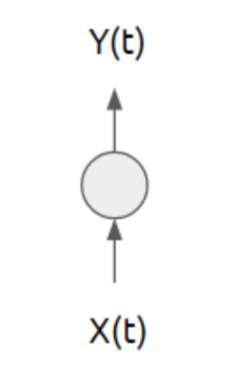
\includegraphics{NNimg1}
        \par
        After fine-tuning the model for a long time you would probably want to test the model in a real-life scenario. Often at times this would be done by calling the model multiple times, maybe repeatedly one after another.
        \par
        The neural network consists of input weights (w in), output weights (w out) and one hidden layer Z(t). The first half of the model would have the formula: Z(t) = X(t) * W in, while the second half of the model would be: Y(t) = Z(t) * W out. 
        
        \subsection{Recurrent Neural Networks (RNN)}\label{recurrrent neural networks}
        {
            The previous section described briefly what pieces a neural network consists of. A recurrent neural network is very similar, but is smarter in a sense. \cite{}.
            \par
            Recurrent Neural Networks (RNN) introduce transition weights to transfer information between time.
            \cite{}.
            \par
            The introduction of transition weights means that the next state is dependent on the previous model, as well as the previous state. This means that the model has memory of what has happened earlier.
            \par
            Recurrent Neural Networks are created to be used with sequential data. Because audio signals are a dimension lower than videos (linear signal vs two-dimensional pixel array) it is a lot easier to get started with audio time series data.
        }
    }
    
    \section{Sequence-to-sequence models for chatbots}\label{sequence-to-sequence models}
    {
        Today real human-beings are hired to work as customer service. To get in touch with this customer service, customers will have to chat online, make phone calls or send e-mails. But these tasks can be automated by developing a software which can interface with the customers by using natural language. \cite{}.
        \par
        Chatbots are receiving a lot of hype due to groundbreaking development in natural language processing thanks to using deep learning techniques. \footnote{Deep learning techniques } Maybe if the chatbot is fed with sufficient amount of training data, it can resolve problems that a lot of customers are dealing with through natural language conversations.\cite{}. 
        \par
        
        \par
        
         \ref{KnowledgeDiscovery}.
    }
    
    \section{Knowledge discovery}\label{KnowledgeDiscovery}
    {
        As described in section \ref{predictive analytics} data are collected constantly, and is not of any value without any form of knowledge extraction. The data in a raw form may not give any valuable information. Knowledge discovery as a process consist of an iterative sequence of the following steps \cite{dataMining}:
        
        \begin{enumerate}\label{}
            \item Data cleaning
            \item Data integration
            \item Data selection
            \item Data transformation
            \item Data mining
            \item Pattern evaluation 
            \item Knowledge presentation
        \end{enumerate}
        The first four steps are different forms of data pre-processing. It is in these steps the data are prepared for data mining, and is illustrated in the figure below \cite{dataMining}.
        
        \begin{figure}[H]
            \centering
            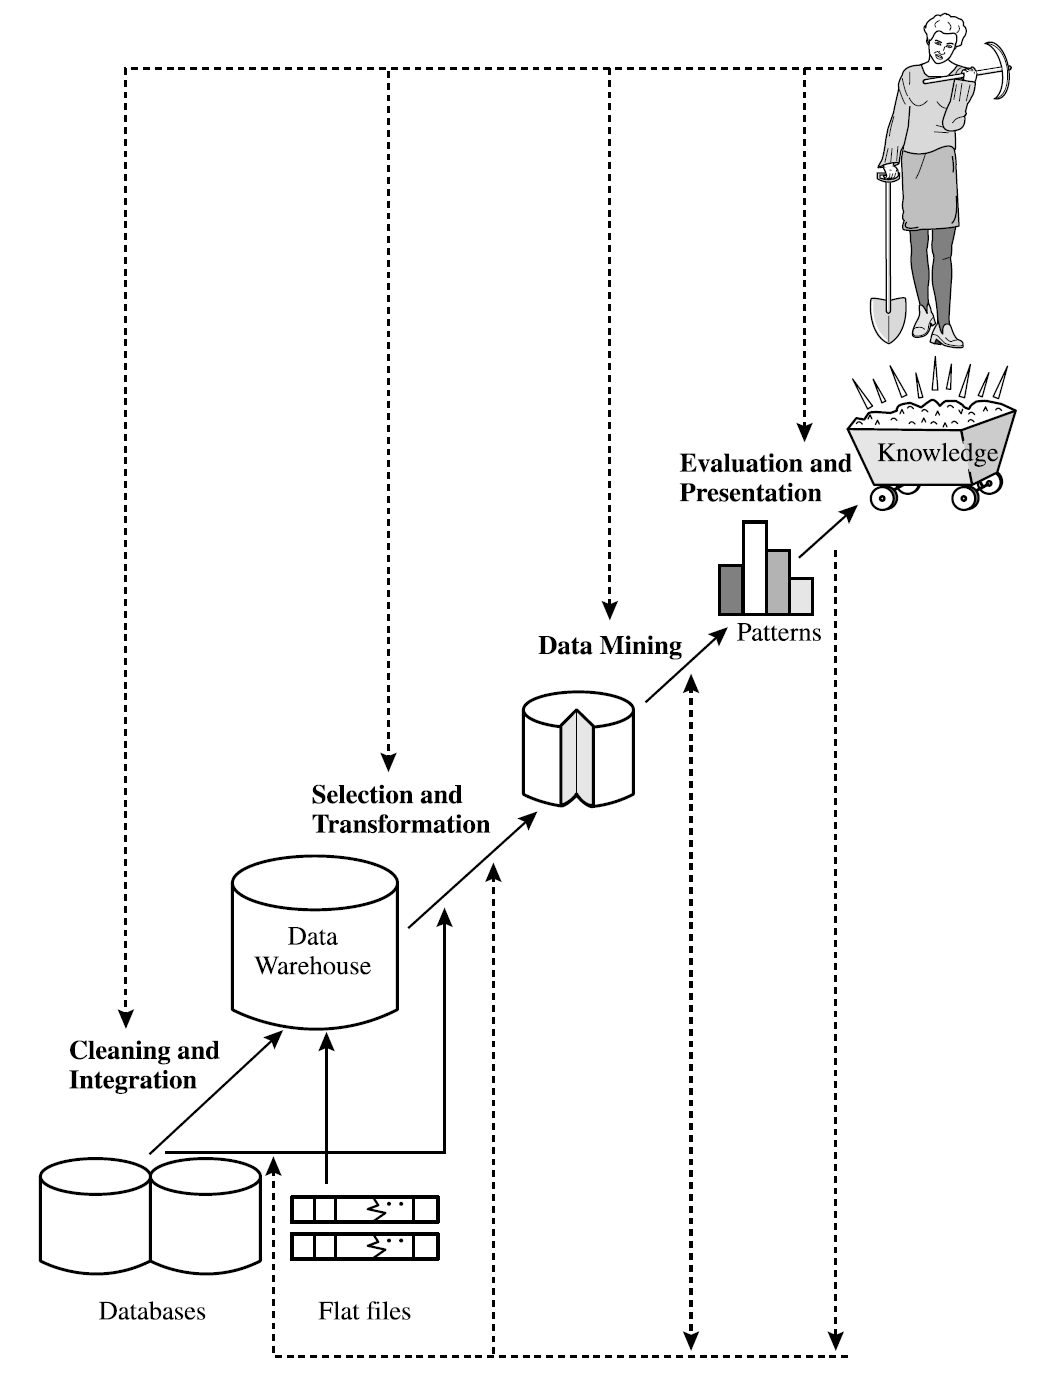
\includegraphics[width=0.5\textwidth]{knowledgeDiscovery}
            \caption{Knowledge discovery \cite{dataMining}}
            \label{fig:knowledgeDiscoverySteps}
        \end{figure}
        
        In \figref{knowledgeDiscoverySteps} the different steps represents:
        \begin{itemize}
            \item \textbf{Databases}. Where the data are stored
            \item \textbf{Data Warehouse}. The data are pre-prosessed
            \item \textbf{Data Mining}. Where intelligent methods are applied
            \item \textbf{Patterns}. Evaluation and presentation
            \item \textbf{Knowldedge}. Useful insights for any user
        \end{itemize}
        The next sections describes pre-prosessing of data.
                
        \subsection{Pre-processing} \label{pre-processing-theory}
        {
            Each system has different machines and sensors, and these produce data. The data collected from the machines and sensors contributes to dimensions of data equal to the sum of data points collected from the system. The pre-processing will essentially transform the raw, real world data to a set of new data. The new data will preserve the valuable information and eliminate at least one of the problems in the raw data \cite{dataPreprocessing}. 
            \par
            Problems in the data may be \cite{dataPreprocessing}:
            
            \begin{itemize}
                \item \textit{Too much data}
                \begin{itemize}
                    \item \textit{Corrupt and noisy data}
                    \par
                    By corrupt data, the quality of the measurement is not reliable. It can arise from transmission failure, sensor failure or logging errors. Noise in the data can come for instance from influence on sensors by external equipment or incomplete data transmission between sensor and logger.
                    
                    \item \textit{Irrelevant data}
                    \par
                    In large datasets some of the data might be irrelevant for the application. Irrelevant data might not contribute to predictions, and by removing the irrelevant data the complexity is reduced, and may improve the performance of the application.
                    \item \textit{Very large data sizes}
                    \par
                    Very large data size are where data is produced at a high rate and in high dimensions. The high number of dimensions and samples can make on-time analysis impossible. Hardware and software might also not be able to handle the analysis of such large amount of data.
                    
                \end{itemize}
                
                \item \textit{Too little data}
                
                \begin{itemize}
                    \item \textit{Missing attributes:}
                    \par
                    Missing attributes in the data represents features with no value and can complicate analysis tasks such as learning and result in inaccurate performance. 
                    
                    \item \textit{Missing attribute values:}
                    \par
                    Missing attribute values is when one or several features is missing some of their values. The missing values can represent information, and therefore can not be eliminated. A decision on what to do with the missing values has to be done. The missing attributes reduces the number of valid data points in the dataset. This might result in a dataset unsuitable for data analysis.
                    
                    \item \textit{Small amount of data:}
                    \par 
                    Small amount of data is when a dataset does not contain enough samples for a proper data analysis, even if there are no missing values.
                    
                \end{itemize}
                
                \item \textit{Fractured data}
                
                \begin{itemize}
                    \item \textit{Incompatible data:}
                    \par 
                    Incompatible data can occur when the data is collected by several groups. Different measure instruments can have different encoding of the sensor readings, and the measurement precision might be different. This can cause that when the data are combined the measurements are incompatible with each other.
                    
                    \item \textit{Multiple sources of data:}
                    \par 
                    If the collected data comes from different sub-systems, the standards, precision, sampling frequency and data storage can vary, and when combined cause problems.
                \end{itemize}
            \end{itemize} 
            
            \subsubsection{Handling missing data}
            {
                In real world datasets we have the probability of missing data by various reasons. The missing data needs to be handled for the machine learning algorithms to perform as they should. If the machine learning algorithms gets missing data points we can not guarantee or predict how the algorithms will handle that scenario \cite{dataPreprocessing}. The missing values can contain valuable information, and therefore a decision has to be made for what to do with the missing data points. 
            }
        }
        
        \subsection{Dimensions in data}
        {
            Dimensions in data tells us how many features the data contains. Each sensor or feature in the system represents its own dimension in the dataset. As an example, a system with five sensors or features will have five dimensions. As more features or sensors are added, the dimensions increase equally.
        }
        
        \subsection{Dimensionality reduction algorithms}
        {
            It is difficult to plot and visualise data with more than three dimensions. As the number of dimensions increases, more training data is necessary. This is known as \textit{the curse of dimensionality}. For many algorithms the dimensionality is an important factor when it comes to the computational cost. These are some reasons why dimensionality reduction can be useful. It can remove noise, improve the results of the learning algorithm, and make the dataset easier to work with and understand. There are three different ways to do dimensionality reduction: feature selection, feature derivation and clustering \cite{mlMarsland}.
            
            \begin{itemize}
                \item \textbf{Feature selection} usually means looking through the available features and checking the correlation with the output variables. 
                \item \textbf{Feature derivation} means deriving new features from the old ones. This is generally done by applying transforms to the dataset that change the axes of the graph. 
                \item \textbf{Clustering} is used to group together similar data points. This is done to see if it can allow fewer features to be used.
            \end{itemize} 
            
            Next we will look at an algorithm for dimensionality reduction.  
        
            \subsubsection{Principle Component Analysis}\label{PCA}
            {
                \gls{pca} is a way of capturing the essence of the original data by compressing a lot of data. The first step finds which direction the data have the largest variation. The next step finds the direction of the second most variation, perpendicular to the first. These steps are repeated for each dimension in the data. For each dimension there will be added a \gls{pc}. That means that \gls{pc}1 will span in the direction with most variation, \gls{pc}2 will span in the direction with 2$^{nd}$ most variation and so on. \\
                After all \gls{pc}s have been decided, it will start looking at which data points have the most influence on each \gls{pc}. The data points on each end of a \gls{pc} will be the ones who influence the most. Based on this it will be set up a table that tells the influence of each data point, and each point will be given a weight. The points in the middle of a \gls{pc} will have values close to 0, while the points at the end of a \gls{pc} will have large values, where one of the ends is positive, while the other is negative. After this, each value of a feature in a data point will be multiplied with the corresponding weight, and thereafter all of these multiplications will be added together. This will tell how much a feature influence a \gls{pc}. Therefore this is repeated for every \gls{pc}. Now we are able to set up a figure with the \gls{pc}s as axes, and this way we will see that similar features will be clustered together \cite{mlMarsland}. 
            }
        }
        
        \subsection{Data transformation} \label{data-transformation-theory}
        {
            When looking at a dataset the different features can have different data types and ranges. The purpose of data transformation is to take the raw data and transform each feature into a given range or to a specific type. The advantages of data transformation comes to play when the data is presented to \gls{ml} algorithms. With data transformation you can guarantee that the data is of a given type and without missing data \cite{dataTransformation}. 
            
            \subsubsection{Normalisation}
            {
                Normalisation is the process of reshaping the data from one range, to a new specified range \cite{scikit-learn-pre-processing}. This range is usually 0 to 1 or -1 to 1, but can be any range. 
            }
        }
    }
    
    \section{Machine Learning}\label{machine learning}
    {
        \subsection{What is machine learning?}\label{what is ml}
        {
             \Gls{ml} is a part of \gls{ai}, that is about developing algorithms that gives computers the ability to learn and adapt from data \cite{artificialIntelligence}. Initially when a machine learning model is built, it has no knowledge. When example data is applied to the model, it will try to adapt to make correct predictions. The target of a machine learning algorithm is to find and use complex patterns in data to make decisions or predictions. 
             \par 
             Machine learning follows a process that involves collecting data, preparing data, train the model, score and evaluate the model and then implement and predict \cite{mlKelleher}. Collecting the data involves either logging necessary data or collecting already logged data from databases or files. The next step regard pre-processing the data. To be able to put useful data into an algorithm the data has to be examined and pre-processed, this is called knowledge discovery. This is to determine which data is useful, what to do with missing data, normalise, extract features and so on. Knowledge discovery was thoroughly explained in section \ref{KnowledgeDiscovery}.
             \par
             When the input data have been pre-processed, training of the machine learning model starts. How the model adapts to the input data depends on the type of machine learning as well as the algorithm. The training process will be explained for the separate algorithms. 
             \par 
             After the training process the model needs to be scored and evaluated. This step involves how to measure the performance of the algorithm and to determine if it sufficiently predicts the target \cite{mlKelleher}. There would be no need to have an algorithm that perform poorer than random guessing. Scoring an algorithm is done in a variety of methods, depending on the target and type. Scoring and evaluation is explained in section \ref{evaluation of algorithms}.
             \par 
             When the model has been evaluated and accepted it can be deployed. A machine learning model is made to serve a purpose, and this step covers the work needed to deploy and maintain the model.
             \par 
             During the process of developing a machine learning model different algorithms can be deployed dependent on the desired result. Machine learning algorithms are usually categorised into four groups \cite{mlMarsland}:     
             \begin{itemize}
                \item \textbf{Supervised learning} is to learn from data that consists of both input and correct target data. The algorithm learns to generalise by adjusting according to the target data to give better predictions.
                \item \textbf{Unsupervised learning} tries to find similarities between input data and cluster or categorise them without having any target data to refer to. 
                \item \textbf{Reinforcement learning} is a combination between supervised and unsupervised learning. A reinforced learning algorithm know when an answer is wrong, but not how to correct it. The algorithm need to explore more solutions in order to get the right one.
                \item \textbf{Evolutionary learning} can be viewed as a learning process inspired by natural selection. Populations are presented and selection, breeding and mutation is performed in order to have the fittest solutions to survive.
            \end{itemize}
            \par
            The most used machine learning algorithm type is supervised learning. Both supervised and unsupervised will be elaborated further in section \ref{supervised learning} and \ref{unsupervised learning} respectively.
        } 
        
        \subsection{Supervised learning}\label{supervised learning}
        {
            Supervised learning is as mentioned in section \ref{what is ml}, a model where examples of input and desired output data are provided. It is called supervised learning since the desired output is provided during the training. Algorithms in this category aim to minimise an external error criterion, like sum-of-squares error. This can be calculated by finding the difference between the output and the targets. Having an error value makes it possible to score an algorithm \cite{mlMarsland}. Supervised learning algorithms are categorised into several sub-types.
            
            \subsubsection{Anomaly detection}\label{anomaly detection}
            {
                Anomaly or outlier means deviation from what is normal, or irregularity from the norm. Anomaly detection is to identify or predict data points, items or events that deviate from the expected pattern. Such anomalies occur infrequently and may be of great importance \cite{mlMarsland}. Examples of this can be to detect credit card fraud or detect abnormal equipment behaviour. There are anomaly detection algorithms for both supervised and unsupervised learning. In order to use supervised learning the datasets must be labelled as normal and abnormal.
            }
            
            \subsubsection{Regression}\label{regressionTheory}
            {
                In statistics, regression is a quantitative analysis of the relationship between one dependent variable and one or more independent variables. It tries to find a mathematical formula that best fits the data. Regression models attempt to model the relationship between variables to predict values. These algorithms use supervised learning to repeatedly adapt the model to better estimate an output value. The output value of a regression algorithm is continuous and numeric \cite{mlMarsland}.
            }
            
            \subsubsection{Classification}\label{classificationTheory}
            {
                Classification models attempts to identify and categorise new data into its corresponding category. A classification problem could be to determine if the object in an image is a car, bus or boat. Such models can differentiate between two categories or several \cite{mlMarsland}.
            }
        }
        
        \subsection{Unsupervised learning}\label{unsupervised learning}
        {
            Unlike supervised learning, unsupervised learning algorithms identifies similarities in data points without having the solution. In many circumstances target data can be difficult to obtain, it might require manually labelling each instance or the target label can even be unknown. This illustrates a fundamental different type of problem than supervised learning since scoring the correctness of a prediction based on the target is impossible \cite{mlMarsland}. 
            \par 
            Unsupervised learning can not perform regression since there is no target data to adapt to. Supervised learning perform classification by finding similarities between inputs that is member of the same class. This requires having the target classes. Unsupervised learning algorithm has no target classes, but can on the other hand find similarities between inputs and cluster them together. The aim of these algorithms is to cluster similar inputs without knowing about the different classes or which class an input belong to \cite{mlMarsland}. 
            \par
            These algorithms can not be scored by calculating any type of error criteria that rely on target data. The scoring of such algorithms need to be dependent on internal factors. This can be done by calculating distance between inputs. If two inputs are close together they are similar and can be clustered together. However if the inputs are far apart they probably belong to different clusters. How these distances are calculated differs from algorithm to algorithm. Euclidean distance is one of these distance measures. The different algorithms are split into categories \cite{mlMarsland}.
            
            \subsubsection{Anomaly detection}
            {
                Anomaly detection has been described in section \ref{supervised learning}. When anomaly detection is used in unsupervised learning unlabelled datasets are used. The algorithms will assume that most of the data is normal and will try to identify outliers or abnormal data points \cite{anomalyDetection}.
            }
            
            \subsubsection{Clustering}
            {
                Clustering has the objective to separate and group similar input data into groups or clusters. This should be done in such a way that objects in one group are more similar to each other than any other group \cite{artificialIntelligence}. Clustering can as an example be used to identify similar areas of land. 
            }
        }
        
        \subsection{What to consider when choosing algorithms}\label{considerationChoosingAlgo}
        {
            When choosing an algorithm there are a lot of considerations to be done. A diversity of machine learning algorithms exists and they have both strengths and weaknesses. In order to solve a desired problem, the chosen machine learning model must predict accurately enough to fulfil the specific problem requirement. Additionally, it is important to explore and accomplish other requirements as well, such as:
            \par 
            \subsubsection{Prediction speed}
            {
                Prediction speed describes how fast a model can make predictions. This could be a crucial factor to be able to solve the desired problem \cite{mlKelleher}. 
            }
            
            \subsubsection{Training time}
            {
                Training time is how much time it takes to train the machine learning model. Some machine learning algorithms are more sensitive when datasets increase in size and therefore training time will increase as well \cite{chooseML}.
            }
            
            \subsubsection{Capacity for retraining}
            {
                When a machine learning model has been implemented it is important to keep monitoring the performance to evaluate if the model has gone stale. If the model has gone stale the model must be changed to adapt and learn according to new scenarios. Some models can be almost impossible to retrain, and a new model needs to be made. However some models can be fairly easy to adapt to new scenarios \cite{mlKelleher}.  
            }
            
            \subsubsection{Interpretability}
            {
                In some situations it is required to get an explanation of why that exact prediction or decision was made. This is called interpretability and is the explanation capability of a machine learning model \cite{mlKelleher}.
            } 
        }
        
        \subsection{Training}\label{training}
        {
            The process of building a machine learning model that predict outputs on new data is called training. The training process depends on the dataset, algorithm and parameters. Supervised learning algorithms typically calculate an error (e.g. mean-square error) between the output and the target and updates weights or similar to change the model \cite{mlKelleher}. Unsupervised learning algorithms have no target to refer to, so these algorithms needs to find and correct themselves by for instance using distances between clusters \cite{artificialIntelligence}. The training processes are different from algorithm to algorithm and will be explained in more detail for each of the relevant algorithms in section \ref{algorithms}.
            \par 
            A common denominator for machine learning algorithms is that the same dataset should not be used for both training and testing. 
            
            \subsubsection{Training, testing and validation set}
            {
                The available dataset used for a machine learning model is divided into three sets:
                
                \begin{itemize}
                    \item Training set is the data used for training a model
                    \item Test set is to evaluate the performance of a model after training.
                    \item Validation set is used to keep track of the performance of a model during training.
                    
                \end{itemize}
                
                The dataset is divided into these individual sets because the same data points should not be used for both training and testing. Using the same data points may lead to an artificially high accuracy due to over-fitting (see section \ref{generalization}). There is no finite solution on how the distribution between the three sets should be. The distribution depends on the diversity and volume of the set. If a lot of data is available a 70:15:15 (70\% for training, 15\% for validation and 15\% for testing) distribution is reasonable, while for smaller sets a 50:25:25 split might be necessary. Different split methods are used, depending on the nature of the dataset. The distribution of the sets can be selected chronological or randomly. In some cases it is necessary to keep the same class ratio in all the sets. This is referred to as stratified split \cite{mlKelleher}. 
                \par
                After a machine learning model has been trained it must be tested and evaluated \cite{artificialIntelligence}.
            }
        }
        
        \subsection{Evaluation}\label{evaluation of algorithms}
        {   
            After a machine learning algorithm has been trained, the prediction model must be tested. This process is referred to as evaluation and deals with methods for scoring the model. The aim of evaluation is to measure the performance of the predictions made from the built models. When several models are built, all of them will be evaluated and compared to find which model performs best to the problem \cite{mlKelleher}.
            \par
            The requirements of a model is not only about how many of the predictions are correct. Some problems might only require better performance than random guessing, while a diagnostic problems require that no sick person is predicted healthy. Performance of a model can be measured in several methods and there are important pitfalls to avoid, such as over-fitting and under-fitting.  
        
            \subsubsection{Generalisation}\label{generalization}
            {
                Generalisation means that a model should not memorise previous input data but learn and extract experience from it. This is called generalisation, and if it is achieved, the model can provide reasonable decisions based on unseen input data. Over-fitting and under-fitting are two terms used when talking about generalisation, and can be the main reasons for bad performance in a machine learning algorithm \cite{mlKelleher}.
                \par
                Over-fitting can be translated to memorising. A lot of data is provided to the algorithm and it runs for several epochs until the input data is memorised. The algorithm performs well on training data, but struggles to make good predictions on new, unseen data. Under-fitting is a model that does not fit the data, and will perform poorly during training and it will not generalise \cite{pythonML}. 
                \par
                
                \begin{figure}[H]
                    \centering 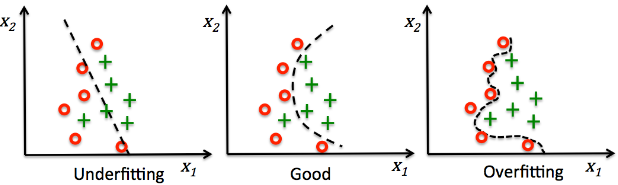
\includegraphics[width=0.8\textwidth]{overunderfitting}
                    \caption{Illustration of over-fitting and under-fitting \cite{pythonML}}
                    \label{fig:overunderfitting}
                \end{figure}
                
                \par
                Another important advantage of generalisation is that even though the input data are noisy (missing or corrupted data) the model might give a correct prediction.
            }
            
            \subsubsection{Confusion matrix}
            {
                A confusion matrix is a way to visualise the performance of a machine learning model. The confusion matrix calculates the frequency of each possible solution from the predictions made for a dataset. Each column shows an instance in a predicted class, while each row shows the actual class. The use of a confusion matrix makes it easier to see if two classes are misclassified \cite{mlKelleher}.
                
                \begin{figure}[H]
                    \centering
                    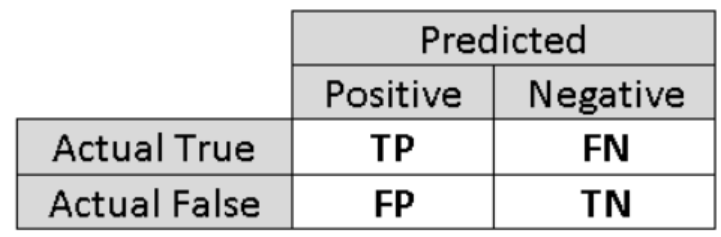
\includegraphics[width=8cm]{ConfusionMatrix}
                    \caption{Structure of a confusion matrix \cite{evaluateML}}
                    \label{fig:ConfusionMatrix}
                \end{figure}
                
                \Figref{ConfusionMatrix} shows the structure of a confusion matrix for a binary classification, where the result is either positive or false. In such a case there are four possible outcomes:
                
                \begin{itemize}
                    \item True Positive (TP): The target is positive, and the prediction is correct (positive). 
                    \item True Negative (TN): The target is negative, and the prediction is correct (negative).
                    \item False Positive (FP): The target is negative, but the prediction is wrong (positive).
                    \item False Negative (FN): The target is positive, but the prediction is wrong (negative).
                \end{itemize}
                
                Confusion matrix visualises which instances that are often misclassified. It also describes two types of misclassifications, false positive (type 1 error) and false negative (type 2 error). Type 1 error indicates that a condition is present when it actually is not. Type 2 error is often more severe misclassification as it indicates that a condition is not present, even tough it is. From a confusion matrix, accuracy and a lot of other useful accuracy metrics can be calculated \cite{mlMarsland}.
            }
            
            \subsubsection{Scoring methods}\label{scoringMethods}
            {   
                Scoring is used to evaluate the predictions. Different methods is used for classification and regression.
                \par 
                In classification, accuracy is often used. Accuracy is the share of correct predictions. If a dataset is unbalanced or the target is to have no type 2 errors, the accuracy measure is not enough. Most scoring methods for classification problems are based on the confusion matrix. If an algorithm should predict normal and dangerous conditions of a system, it could be deceptive to measure percentage of correct predictions. These can be misleading if the system is in normal condition 99,9\% of the time and the algorithm only predict this condition \cite{mlKelleher}. There are a lot of different scoring metrics for classification problems, and the scoring method must be chosen based on the particular problem.
                \par 
                Scoring of regression models cannot be done with the same metrics as classification problems. The scoring of regression models tells something about the difference between the predictions and the actual output. One example of a scoring metric for regression algorithms is \gls{mse}, which is the average of the squared errors between the target and the predictions. This means that the error is squared to avoid negative values, summed together and then the average of these values is considered the \gls{mse} \cite{mlKelleher}. A variety of methods for scoring regression predictions exist, and they must be chosen based on the particular problem, just like the classification scoring.
                \par 
                The different scoring methods will be explained in section \ref{methods-for-scoring}. 
            }
        }
        
        \subsection{Deployment} \label{deployment}
        {
            After a machine learning model have been chosen based on the evaluation, the next step is to deploy the model. Deployment is the part where a machine learning model fulfils its purpose in an organisation. Deployment includes the necessary steps to utilise and maintain a machine learning model \cite{mlKelleher}. It is important that such a model is maintainable, and can remain accurate. 
            \par
            
            A machine learning model can be made from scratch by programming or by the means of tools such as Microsoft Azure Machine Learning platform (see section \ref{microsoft azure}). These models can be deployed as a software integrated to already existing systems or as a web service. 

            \subsubsection{Utilise}
            {
                An important step when utilising a machine learning model is to specify the performance requirements. These requirements can be a range of performance expectation or a minimum accuracy value. Having these requirements makes it easier to test the model, and decide if it still performs as expected or if retraining is necessary \cite{mlMarsland}. 
            }
            
            \subsubsection{Maintain}
            {
                A machine learning model must be maintained to keep the performance within the requirements. A model is rarely static, and need to retrain as new data are available or data and other factor changes. The retraining process can be done regularly by retraining the system with new data, evaluate the system and then make the update available \cite{deployML}. 
            }
        }
    }
    
    \section{Machine learning (ML) algorithms}\label{algorithms}
    {
        This chapter deals with more detailed explanations of the machine learning algorithms relevant in this project.
        
        \subsection{Artificial Neural Network (ANN)}\label{annTheroy}
        {
            \gls{ann} is one of the most popular approaches to machine learning, and can be supervised, unsupervised or a reinforcement learning algorithm according to Negnevitsky \cite{artificialIntelligence}. In his book he explains how an artificial neural network can be defined as a model of reasoning based on the human brain. Just like the biological neural network, the \gls{ann} consists of a lot simple and interconnected processors, called neurons. These neurons are connected together by weighted connections that can pass signals in between them. Each neuron can have multiple input signals, but only one output which can be distributed to several new neurons. \Figref{NeuronDiagram} shows a single neuron with input signals, weights and output signals.  
            \par
            
            \begin{figure}[H]
                \centering
                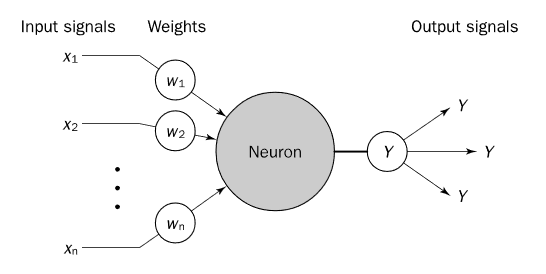
\includegraphics[width=0.65\textwidth]{NeuronDiagram}
                \caption{Simple architecture of a neuron in an \gls{ann} \cite{artificialIntelligence}}
                \label{fig:NeuronDiagram}
            \end{figure}
            
            \par
            A neuron has several weighted inputs, from these it computes its activation level which is the neurons output that will either be an input to another neuron or the final output of the neural network. The activation level is determined from an activation function in the neuron. These functions can be hard-limiters such as a step or sign function, where the output will be one of two values based on if a certain threshold is reached. These activation functions are typically used for classification problems, while regression problems could use functions such as sigmoid or linear activation. The sigmoid activation function is typically used in back-propagation networks and transforms the input number into a number between 0 and 1. 
            \par
            The ability to learn is what makes the \gls{ann} intelligent and popular. Every connection between the neurons has a numerical weight associated with it and they are the memory part of an \gls{ann}. Through repeated training these weights will be adjusted and represent the importance of each input into a neuron.
            A typical \gls{ann} has two phases, a forward pass and a backward pass, as showed in \figref{twoPhaseNN}.
            
            \begin{figure}[H]
                \centering
                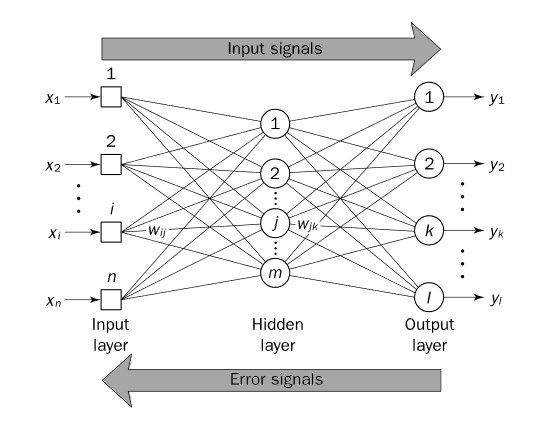
\includegraphics[width=0.6\textwidth]{twoPhaseNN}
                \caption{\gls{ann} architecture with forward and backward pass \cite{artificialIntelligence}}
                \label{fig:twoPhaseNN}
            \end{figure}
            
            \par    
            A lot of different algorithms for training exists for \gls{ann}. Typically, the forward pass calculates output of each neuron until the network output is reached. In supervised learning the difference between the actual output and the predicted output is calculated, called the error. It is back-propagated through the network to every layer and neuron. The back-propagated error is used to find the gradient descent which again is used to update the weights. The gradient descent simplifies finding the minimum of the error, but it can get stuck in a local minimum. These types of learning algorithms are called back-propagation algorithms and uses the gradient descent as an optimisation method for adjusting the network weights for minimising the error \cite{makeNeuralNetwork}.
            \par
            An \gls{ann} exists in a wide variety of types and is typically used for regression or classification problems (see section \ref{classificationTheory}). Both these kinds of problems are based on supervised learning, but an \gls{ann} can also be used for unsupervised learning and thus clustering problems. For these kinds of problems, the network cannot adjust the weights according to the error during the training, and a different approach is necessary. A number of clusters must be specified, and an equal amount of centroid will be randomly generated. When training samples are provided to the network, the sample will be assigned to the closest centroid. For each provided sample, a new centroid will be calculated based on previous assigned samples \cite{artificialIntelligence}.
            
            \subsubsection{Multilayer perceptron}\label{mlp}
            {
                Multilayer perceptron is a supervised learning implementation of an \gls{ann} that can be used for both classification and regression problems. It is a feedforward \gls{ann} with multiple layers of nodes, fully connected to each other. The \gls{mlp} is able to learn non-linear connection, and uses the mentioned back-propagation algorithm to update the weights. The number of layers, nodes in each layer and the type of activation function are some of the necessary settings of the \gls{mlp} \cite{artificialIntelligence}.
            }
        }

        \subsection{Support Vector Machines (SVM)}\label{svmTheory}
        {            
            \Gls{svm} is a \gls{ml} algorithm that can be used for both classification and regression problems. A \gls{svm} is normally a supervised learning model, but has variants that can be used for unsupervised learning, such as the One-class \gls{svm}.
            \par
            The most common approach of a \gls{ml} algorithm is to learn from data, and try to generalise and find the most common combinations between inputs and outputs. The \gls{svm} tries to find n-dimensional support vectors which can divide the data. This is a slightly different approach than other \gls{ml} algorithms as the \gls{svm} tries to find the most uncommon points in a cluster and use it as support vectors \cite{pracGuideSVM}. Basically this means that the \gls{svm} tries to maximise the distance between the different classes' support vectors, as shown in \figref{SVM-easy}, where the filled points are the support vectors and the hyperplane is used for classifying points from the two inputs, X1 and X2, from each other. 
            \par
            In general, there are three main parameters to fit the \gls{svm}s, 'C', 'kernel' and '\begin{math} \gamma \end{math}'. There is one fourth parameter that is used in a sub-type of the \gls{svm}, the \acrshort{ocsvm}. This parameter is an offspring of the 'C' parameter, and is called '\begin{math} \nu \end{math}'. From the \gls{skl} documentation we find that the parameters are defined as described in the coming paragraphs \cite{scikit-learn}, and from the book Learning with kernels, we describe the 'kernel' function \cite{scholkopf2002learning}, in short.
            \par
            The \textbf{C} parameter can be interpreted as a smoothness of the decision line, but is actually a trade-off between the model complexity and the number of training errors. The C parameter has a range of 0 to \begin{math} \infty \end{math}, where as the \textbf{\begin{math} \nu \end{math}} parameter has the range 0 to 1, and is a fraction instead of a number.
            \par
            \textbf{Kernel} is a similarity function, which calculates the similarity over data points, and \textbf{\begin{math} \gamma \end{math}} is a kernel coefficient used for some types of kernels.         
            
            \begin{figure}[H]
                \centering
                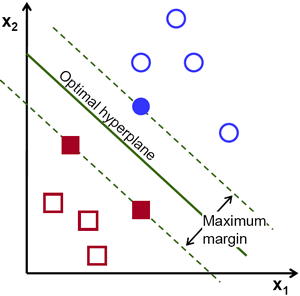
\includegraphics[width=0.4\textwidth]{SVM-easy}
                \caption{Illustration of \gls{svm} principals with hyperplane \cite{openCV-SVMfig}}
                \label{fig:SVM-easy}
            \end{figure}
            
            \subsubsection{SVR}
            {
                Support vector regression or \gls{svm} regression, is a support vector algorithm designed for regression problems. Instead of estimating hyperplane for class separation as with the \gls{svm} for classification, it estimates a hyperplane that fits the training data as good as possible, with a maximum error of \begin{math} \epsilon \end{math} \cite{guideSVR}, shown in \figref{SVR-easy}.
                
                \begin{figure}[H]
                    \centering 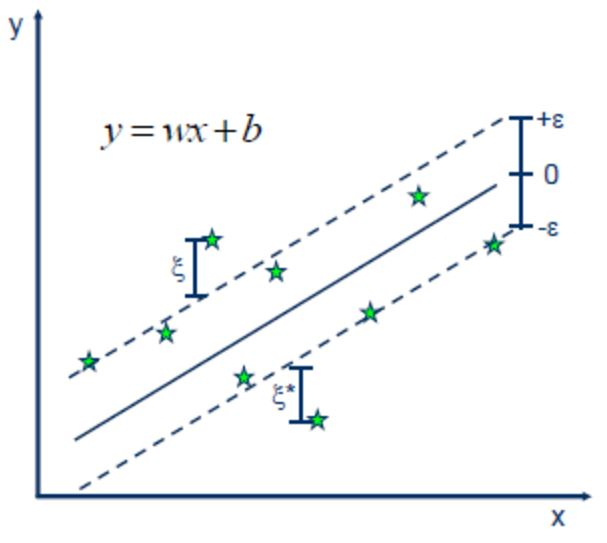
\includegraphics[width=0.4\textwidth]{e-svr}
                    \caption{Illustration of SVR principals with estimation \cite{introSVR}}
                    \label{fig:SVR-easy}
                \end{figure}
            }
            
            \subsubsection{One-class SVM} \label{oneclassSVM}
            {   
                In contrast to the typical \gls{svm}, \gls{ocsvm} is an unsupervised \gls{ml} technique. \textit{"Unsupervised algorithms are algorithms that learns a decision function for novelty detection: classifying new data as similar or different to the training set"} \cite{scikit-learn}. The decision function is a way to generalise the \gls{ocsvm}'s knowledge of the seen points, to estimate a new point's similarity to the seen points from the training data. The generalisation can be adjusted by fine-tuning the parameters, to yield a certain error in the training set predictions, as explained above. 
            }
        }
        
        \subsection{Decision Tree}\label{DecisionTreeTheory}
        {
            Decision tree is a type of \gls{ml} technique that can be used for either classification or regression models. It is often mentioned as a decision support tool. A decision tree basically tries to build a model based on tree structure. It consists of a root node (starting node), interior nodes and leaf nodes that are connected with branches. Root node and interior nodes is specific tests to perform on an available feature. By following the branches and tests in a decision tree, eventually a leaf node is reached. Leaf node is the final node and represents the prediction from the tree. The depth of a decision tree indicate the length of the longest path between root and leaf node. A deeper tree, can have more complex decision rules. Often, implementations of decision trees require a specified max depth \cite{mlKelleher}. \Figref{DecisionTreeExample} shows an example of a simple decision tree \cite{mlInPython}. Leaf nodes is represented as circles, root and interior nodes as rectangles and branches as arrows. 
            
            \begin{figure}[H]
                \centering
                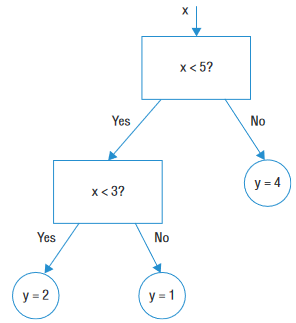
\includegraphics[width=0.45\textwidth]{DecisionTreeExample}
                \caption{Example of a simple decision tree \cite{mlInPython}}
                \label{fig:DecisionTreeExample}
            \end{figure}   
        }
        
        \subsection{Random Forest}\label{RandomForestTheory}
        {
            Random forest is a version of ensemble learning used to build \gls{ml} models. The principle of ensemble learning is that taking the average of several predictions can improve a prediction. In practice this means that a collection of models is built, each model make a prediction and for classification the class with the most votes is the prediction, while for regression problems it is the average of all predictions \cite{pythonML}.
            \par
            The random forest algorithm picks random data points from the training set, and builds a decision tree (section \ref{DecisionTreeTheory}) associated with these data points.  This process is repeated until N trees are built. When new data points is applied to the random forest, each tree predict an output level, and assign a prediction based on voting or average. This approach of building models is referred to as bagging (bootstrap aggregating). Random forest is in other words prediction based on several decision trees, and emphasises that stronger decision are made when supported by several trees. The model is more redundant as it is not as vulnerable if one tree performs badly \cite{mlInPython}.
        }
        
        \subsection{Gradient Boosting}\label{GradientBoostingTheory}
        {
            Gradient boosting is a \gls{ml} technique that can be used both for regression and classification. Just like random forest (see section \ref{RandomForestTheory}) gradient boosting is an ensemble technique, but uses another technique for selecting the models in the ensemble, called boosting. In boosting each subsequent model in the ensemble aims to perform better where the previous model performed badly. Gradient boosting algorithm can use different models in the ensemble, but typically decision trees (section \ref{DecisionTreeTheory}) are used \cite{mlInPython}.
            \par
            The strength of such an ensemble is that all the models in the ensemble make predictions and voting (classifier) or average (regression) is performed on the predictions and the result is the final prediction \cite{mlInPython}.  
        }
        
        \subsection{Adaptive Boosting}\label{AdaBoostTheory}
        {
            Adaptive boosting is another machine learning technique that can be used for either regression or classification problems. It is also of the ensemble type, and is often referred to as AdaBoost. The technique is based on the same principles as the gradient boosting since each model tries to perform better on the instances that previous models has mis-classified \cite{understandingMLAlgos}. Basis for the technique is that a set of weak learners (slightly better than random guessing) can perform better together. The type of model in the ensemble can vary, one standard approach is using the decision trees (section \ref{DecisionTreeTheory}). AdaBoost is sensitive for datasets with noise and outliers \cite{pythonML}.    
        }
        
        \subsection{K-means clustering}\label{K-MeansClusteringTheory}
        {
            K-means clustering is an unsupervised \gls{ml} algorithm that can cluster data points in to a specified number, \textbf{K}, of clusters. The idea behind a clustering algorithm such as this, is to find clusters or groups in a dataset that you might not know exist \cite{pythonML}. 
            \par
            The algorithm aims to divide the data into K clusters, thus K centroids are randomly chosen. All the data points are assigned to the closest centroid based on a distance measure like for instance the Euclidian distance. These data points form the clusters, and from these points new centroid positions is calculated. The data points are then reassigned to the new clusters, again based on distance. If all the data point still are assigned to the same clusters the algorithm have converged and there is no need for further training. Alternatively, if some data points are reassigned new cluster centroids are calculated. This process is repeated until the algorithm converges or an maximum number of iterations is reached \cite{pythonML}.
        }
        
        \subsection{Linear models}\label{LinearModelsTheory}
        {
            Linear models can be used for both regression and classification. 
        
            Linear regression is a statistical approach for modelling the relation between one or several inputs ($x_i$) and an output y.  Simplified, this signify finding the best-fitting straight line through a set of samples \cite{pythonML}. Simple linear regression is finding the best fitting line through a set of samples with only one dependency parameter between the input and the output. It is given by the formula:
            
            \begin{equation}\label{SimpleLinearRegression}
                Y=b_0 + b_1 * x
            \end{equation}
            
            where Y is the dependent variable, x is independent variable and b is coefficients. The coefficients are adjusted until the line best fits the data. The target is to find a linear correlation between x and Y \cite{pythonML}.
            \par
            The simple linear regression finds the best fitting line by using the ordinary least square method (OLS), which aims to minimise the sum of vertical squared errors.  The sum of vertical squared error is the difference between an observation and a prediction from the linear model, squared. The OLS method uses an optimisation algorithm like for instance the gradient descent to minimise the vertical squared error. OLS is sensitive for outliers and can perform poorly with many variables and dependencies between variables \cite{scikitGeneralisedLinMod}. Equation \ref{SimpleLinearRegression} was an example of a simple linear regression, but the OLS can just as easy be used with several independent variables (x-values).
            \par
            Other types of linear models that addresses the problems of the OLS method, exists. They use other cost functions and introduce regularisation\footnote{In \gls{ml}, regularisation is a process of adding information to attempt to avoid over-fitting as well as solving other ill-posed problems} methods. Some examples is listed below \cite{scikitGeneralisedLinMod}:
            \begin{itemize}
                \item Ridge regression
                \item LASSO regression
                \item Elastic net regression
                \item Logistic regression
                \item SGD regression
            \end{itemize}
            
            To be able to use linear models for classification, the linear regression algorithm need to be generalised. This means that equation \ref{SimpleLinearRegression} will be combined with an activation function. Not all generalised linear models are suited for classification, but logistic regression and SGD regression are two of the models that can be used for both regression and classification \cite{scikitGeneralisedLinMod}. 
        }
        
        \subsection{Nearest neighbour (NN)} \label{nearest-neighbour}
        {
            The \gls{nn} algorithm is used for classification, and is known as a lazy learning algorithm. The reason for this is that it stores all the training examples and classifies new instances by finding the closest training example to the new instance. To find the closest training example the Euclidean distance (equation \ref{euclideanDistance}) is used \cite{nearestneighbour}.
            
            \begin{equation}\label{euclideanDistance}
                ||x-x_i||=\sqrt{\sum_j(x_j-x_{ij})^2}
            \end{equation}
            
            \subsubsection{k-Nearest Neighbour (kNN)}\label{knnTheory}
            {
                \gls{knn} is an improvement of the \gls{nn} algorithm, and can be used in classification and regression problems. The improvement of \gls{knn} in respect to \gls{nn} is that \gls{knn} uses the k nearest instances from the training data to predict the output. A \gls{knn} algorithm with a k value of 1, can be considered a \gls{nn} algorithm where only the nearest training instance will contribute to the output.\par
                
                \begin{itemize}
                    \item When using the \gls{knn} algorithm for classification the predicted output is a class membership, and will be classified by the vote majority of the k nearest instances in the training examples.
                    \item When using the \gls{knn} algorithm for regression the predicted output is a property value for the object, and will be the average of the values of the k nearest instances in the training examples.
                \end{itemize}
                
                There are different approaches for computing the nearest neighbours \cite{nearestneighbourAlgorithm}:
                
                \begin{itemize}
                    \item \textbf{Brute force:} \par The brute force method for computing the nearest neighbours is to calculate the distance to all pairs of points in the training-dataset, and predict on the k smallest distances of these. The algorithm in this case stores the whole training-dataset, and therefore is fast to train, but slow to predict. The computation for \textit{N} samples in \textit{D} dimensions scales as:
                    \begin{equation}
                        O[DN^2]
                    \end{equation}
                    A disadvantage of the brute force method, beside long computational time on large dataset, is that it requires a lot of memory to store big training dataset, and memory errors can occur.
                    \item \textbf{K-D Tree:} \par The K-D tree method for computing the nearest neighbours addresses the brute force method by structure information of the distances to each neighbour in a tree-based data structure. The basic idea is that if the distance between point \textit{A} and \textit{B} is large, and the distance between point \textit{C} and \textit{B} is small, we know that the distance between point \textit{A} and \textit{C} is large. 
                    \par 
                    The tree is constructed by dividing the dataset along its Cartesian axis with straight lines. Once the tree is constructed, the number of nearest neighbour distance computation for a query point can be determined by:
                    \begin{equation}
                        O[log(N)]
                    \end{equation}
                    The K-D tree method is very fast for low dimension neighbour search, \textit{(D $<$ 20)}, but becomes inefficient as \textit{D} becomes very large.
                    \item \textbf{Ball Tree:} \par The Ball tree method addresses the inefficiency of K-D tree for high dimension neighbour search. Where the K-D tree method divides the data its along Cartesian axes with straight lines, the Ball tree method partitions data in a series of nesting hyper-spheres. This approach is more computational costly compared to K-D tree, but results in a data structure that can be very efficient on highly structured data, even in very high dimensions.
                \end{itemize}
            }
        }
        
        \subsection{Naive Bayes} \label{naiveBayesTheory}
        {
            Naive Bayes methods are supervised algorithms based on the Bayes' theorem, which is shown in equation \ref{bayesTheorem}:
            
            \begin{equation} \label{bayesTheorem}
                P(y|x_1,...,x_n) = \frac{P(y)P(x_1,...,x_n|y)}{P(x_1,...,x_n)}
            \end{equation}
            
            where \begin{math} y \end{math} is a class variable and \begin{math} x_1 \end{math} through \begin{math} x_n \end{math} is a dependent feature vector.
            \par 
            The reason why it is called Naive Bayes is that the algorithms assumes that every pair of features in the dependent feature vector is independent. This can be written as in equation \ref{}:
            
            \begin{equation}
                P(x_i|y,x_1,...,x_{i-1},x_{i+1},...,x_n) = P(x_i|y)
            \end{equation}
            
            The main difference between the different naive Bayes classifiers is that they have different assumptions when it comes to the distribution of \begin{math} P(x_i|y) \end{math} \cite{scikitNaiveBayes}.
            \par 
            In principle, this means that the naive Bayes methods calculate the probabilities of a data point belonging to each of the classes. Then it classifies the data point to the class with the highest probability. 
        }
    }
    
    \section{Anomalies} \label{anomaliesTheory}
    {
        \subsection{What are anomalies?} \label{whatAreAnomalies}
        {
            Anomaly means deviation from what is expected or irregularity from the norm. Anomaly detection is the problem of finding patterns in data that do not behave has expected. Another word for anomalies are outliers, and these are often used interchangeably. 
            \par
            
            \begin{figure}[H]
                \centering
                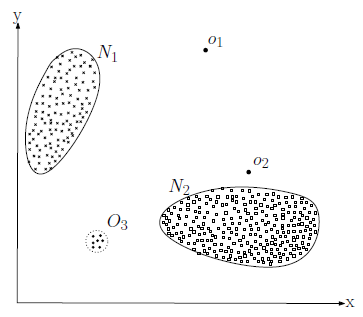
\includegraphics[width=0.5\textwidth]{anomalies}
                \caption{Example of anomalies in a 2-dimensional dataset \cite{anomalyDetection}}
                \label{fig:anomalies}
            \end{figure} 
            
            \par
            As seen in \figref{anomalies} there are two normal regions, $N_{1}$ and $N_{2}$. A normal region is defined by where most observations lie. If a point, or a region of points, is far enough away from the normal regions, these can be considered as anomalies. In the figure there are two points, $o_{1}$ and $o_{2}$, as well as a region of points, $O_{3}$, that can be considered as anomalies. The reason why an anomaly occur is a key feature of anomaly detection \cite{anomalyDetection}. 
        }
        
        \subsection{Definitions}\label{anomDefinitions}
        {
            As mentioned, the reason why an anomaly occur is important to be able to choose the correct anomaly detection technique. Anomalies can be divided into three categories: point, contextual and collective anomalies \cite{anomalyDetection}. 
            
            \subsubsection{Point Anomalies}
            {
                A point anomaly is the simplest type of anomaly. It occurs if an individual point in the data can be considered as anomalous compared with the rest of the data. If we take a look at \figref{anomalies} again we can see that $o_{1}$ and $o_{2}$ as well as points in the region $O_{3}$ can be considered as point anomalies since they are different than the normal regions \cite{anomalyDetection}. 
            }
            
            \subsubsection{Contextual Anomalies} \label{contextualAnomaly}
            {
                An anomaly can be considered as an anomaly if it is an anomaly only in a specific context, but not otherwise. This is what we call a contextual anomaly. A context has to be specified as a part of the problem, as the notion of a context is induced by the structure in the dataset. Therefore each instance in the dataset need to be defined using two sets of attributes:
                
                \begin{itemize}
                    \item \textit{Contextual attributes:} These attributes are used to determine the context of the specific instance. 
                    \item \textit{Behavioral attributes:} These attributes define the non-contextual characteristics of the specific instance. 
                \end{itemize}
                
                When looking at the behavioral attributes of a data instance within a specific context you can determine the anomalous behavior. In a dataset there can be two identical instances where one of them is an anomaly while the other is not at a given time. This is very important for a contextual anomaly detection technique to identify the contextual and behavioral attributes. 
                \par
                
                \begin{figure}[H]
                    \centering
                    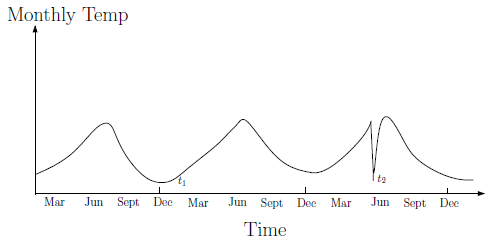
\includegraphics{contextualAnomaly}
                    \caption{Example of a contextual anomaly \cite{anomalyDetection}}
                    \label{fig:contextualAnomaly}
                \end{figure} 
                
                \par
                As seen in \figref{contextualAnomaly} $t_1$ and $t_2$ is the same temperature, but while $t_1$ is considered a normal temperature in February/March, $t_2$ is not considered as a normal temperature in June \cite{anomalyDetection}. 
            }
            
            \subsubsection{Collective Anomalies}
            {
                A collective anomaly occurs when a collection of data instances is anomalous compared to the rest of the dataset. A single data instance from this collection do not necessarily have to be an anomaly by its own, but when these anomalies occur as a collection they are anomalous. Data instances in a dataset have to be related for a collective anomaly to occur \cite{anomalyDetection}. 
            }
        }
    }
    
    \section{Time Series Anomalies} \label{anomalyDetectionTimeSeries}
    {
        Sometimes data instances can be related to each other. When instances are related to each other the data have been collected as sequences or time series. An example of this is when you have a system where you read data from sensors. If your system fail, one or several sensors can have an anomalous reading compared to normal. \\
        As mentioned earlier, an anomaly in data points occurs when you have an unusual value. The difference when looking at sequential data is that a single value do not necessarily have to be an anomaly, but if that same value occurs for an abnormally long time it is an anomaly. If you do not consider the time in a case like this, the anomaly will never be detected as the value itself is not an anomaly \cite{anomalyDetectionOfTimeSeries}.
        
        \begin{figure}[H]
            \centering
            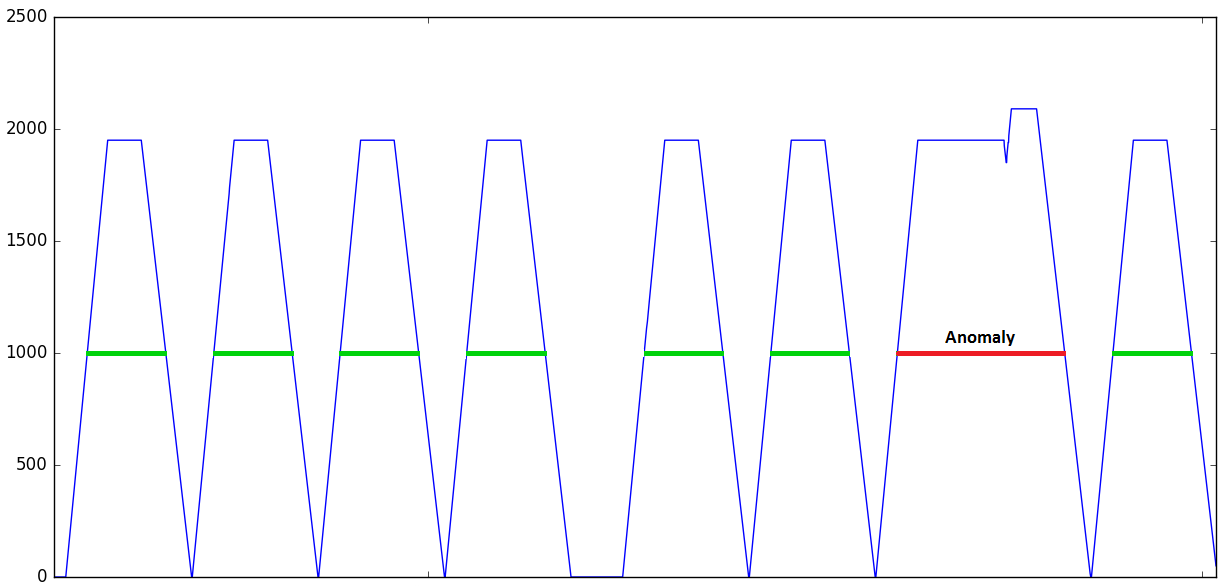
\includegraphics[width=\textwidth]{timeSeriesAnomaly}
            \caption{Example of a time series anomaly}
            \label{fig:timeSeriesAD}
        \end{figure}
        
        As seen in \figref{timeSeriesAD} there is a normal state (the green lines). Suddenly this state continues for a longer time than it usually does, then it is considered as an anomaly.
        
        \subsection{Definitions}
        {
            As with anomalies in data points, anomalies in time series data also have different definitions/categories \cite{anomalyDetectionOfTimeSeries}.
            
            \subsubsection{Contextual anomalies}
            {
                As in section \ref{contextualAnomaly} a contextual anomaly in time series data is an anomaly only in a specific context, not otherwise. See \figref{contextualAnomaly}.
            }
            
            \subsubsection{Anomalous subsequence}
            {
                Another way to define an anomaly in time series is when a subsequence is an anomaly compared to a given long sequence. \Figref{timeSeriesAD} is an example of this, as the last sequence is an anomaly compared to the rest of the time series.
            }
            
            \subsubsection{Anomalous time series}
            {
                The third definition is when an entire time series is an anomaly compared to a time series of normal data. This can be used for unsupervised learning, where you have a training dataset in a database that consist of mostly normal data. This dataset get compared with your new data, and if your dataset is different from your training data you have an anomaly. 
            }
        }
        
        \subsection{Types}\label{anomTimeTypes}
        {
            When talking about time series data there are two characteristics you need to have knowledge about, periodicity and synchronisation. The combination of these two characteristics give 4 different types of time series for a given dataset with \textit{n} normal time series \cite{anomalyDetectionOfTimeSeries}.
            
            \subsubsection{Periodic and Synchronous}
            {
                In this case each time series have a constant time period and every time series is synchronous. That means that they are temporally aligned/start at the same time.
                
                \begin{figure}[H]
                    \centering 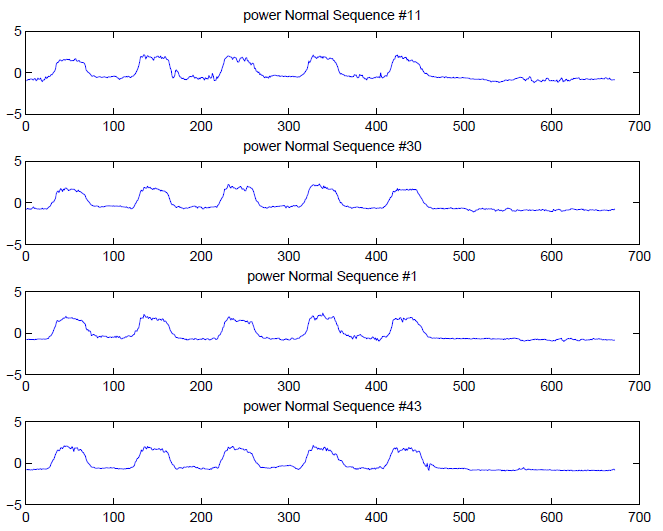
\includegraphics[width=0.5\textwidth]{periodicSynchronous}
                    \caption{Periodic and Synchronous time series \cite{anomalyDetectionOfTimeSeries}}
                    \label{fig:periodicSynchronous}
                \end{figure}
            }
            
            \subsubsection{Aperiodic and Synchronous}
            {
                This means that each time series do not have a constant time period, but they are synchronous.
                
                \begin{figure}[H]
                    \centering 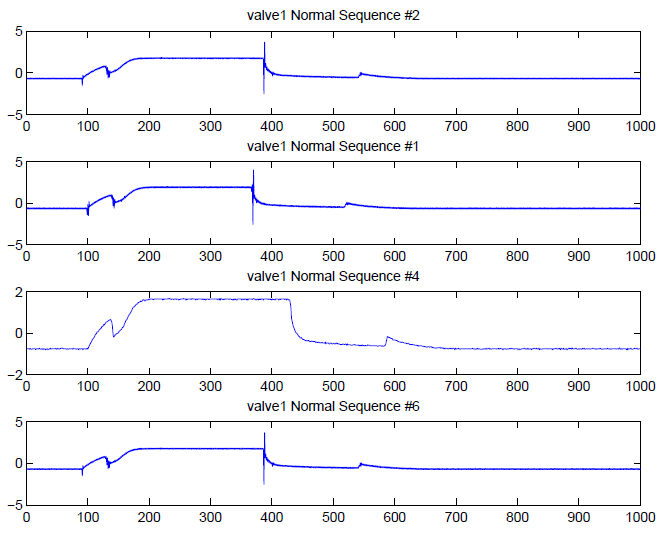
\includegraphics[width=0.5\textwidth]{aperiodicSynchronous}
                    \caption{Aperiodic and Synchronous time series \cite{anomalyDetectionOfTimeSeries}}
                    \label{fig:aperiodicSynchronous}
                \end{figure}
            }
            
            \subsubsection{Periodic and Asynchronous}
            {
                In this case each time series have a constant time period, but they are not synchronous. That means that they do not necessarily start at the same time.
                
                \begin{figure}[H]
                    \centering 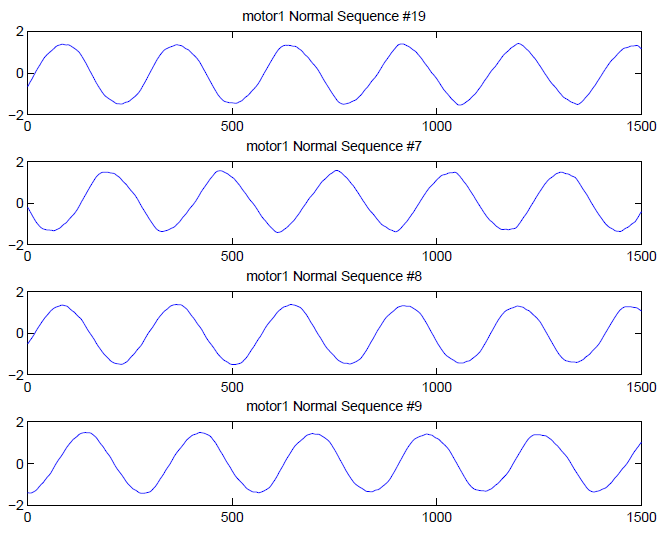
\includegraphics[width=0.5\textwidth]{periodicAsynchronous}
                    \caption{Periodic and Asynchronous time series \cite{anomalyDetectionOfTimeSeries}}
                    \label{fig:periodicAsynchronous}
                \end{figure}
            }
            
            \subsubsection{Aperiodic and Asynchronous}
            {
                This means that they neither have a constant time period nor start at the same time.
                
                \begin{figure}[H]
                    \centering 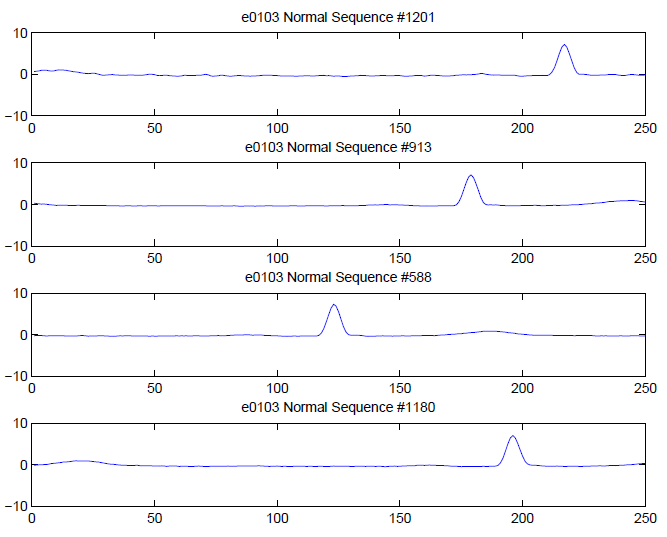
\includegraphics[width=0.5\textwidth]{aperiodicAsynchronous}
                    \caption{Aperiodic and Asynchronous time series \cite{anomalyDetectionOfTimeSeries}}
                    \label{fig:aperiodicAsynchronous}
                \end{figure}
            }
        }
    }
    
    \section{Anomaly Detection} \label{anomalyDetection}
    {
        As mentioned in section \ref{whatAreAnomalies} anomaly detection is the problem of finding patterns in data that do not behave as expected. The reason why anomaly detection is of big interest is that an anomaly can cause a significant, and often critical, incident in many applications \cite{anomalyDetection}. An example of an anomaly detection system is Microsoft's log-in system. If you log-in to your Microsoft account from another country or from a new device, you will get an email from Microsoft where they notify you of an unusual account activity. That is because your log-in have been considered as an anomaly. 
        
        \subsection{Challenges} \label{anomDetChallenges}
        {
            The definition of an anomaly is quite easy to understand, but there are several factors that makes it difficult to find a straightforward anomaly detection approach \cite{anomalyDetection}. 
            
            \begin{itemize}
                \item As mentioned in section \ref{whatAreAnomalies} we have one or several normal regions, but defining these regions so that they surround every possible normal behaviour is very difficult. Also, the limits between a normal and an anomalous behaviour can often be imprecise. This is something that can cause an observation that lies close to the normal regions to be identified as an anomalous behaviour, but it could actually be a normal one. 
                \item If an anomaly is caused by a malicious action, the one who is carrying out the malicious action try to constantly adapt to make the anomaly appear as a normal observation. 
                \item The definition of a normal behaviour can change with time in some applications.
                \item How much offset/deviation of an observation that is accepted before it can be considered as an anomaly is often different from one application to another. Therefore you can not necessarily use the same anomaly detection technique on two different applications. 
                \item When it comes to training/validation of a model that is used for anomaly detection there is not always sufficient labelled data available. 
                \item Very often data contains noise. This noise can sometimes be similar to the anomalies, and therefore not easy to remove. 
            \end{itemize}
            
            \par
            These challenges are reasons why anomaly detection is not easy. There is already a lot of techniques for this, but most often they are made for a specific part of a problem. Which parts of a problem that is covered is decided by several factors: nature of data, availability of labelled data, what kind of anomalies to be detected etc. Because these factors can be difficult to obtain, researchers have made a general method that shows the key components of how to develop an anomaly detection technique \cite{anomalyDetection}.
            
            \begin{figure}[H]
                \centering 
                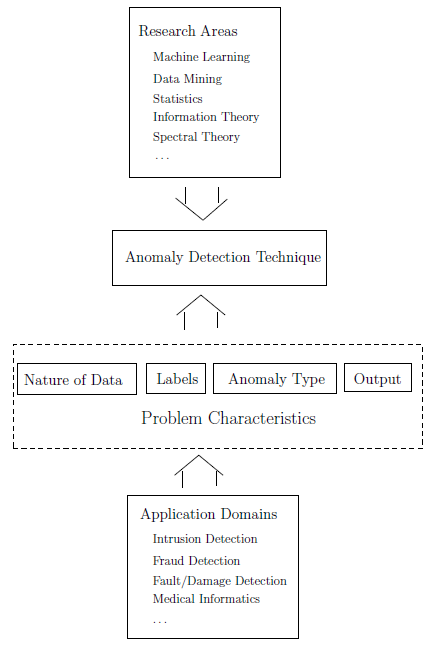
\includegraphics[width=0.5\textwidth]{anomalyDetectionTechnique}
                \caption{Key components in developing an anomaly detection technique \cite{anomalyDetection}}
                \label{fig:anomalyDetectionTechnique}
            \end{figure}
        }
        
        As seen in \figref{anomalyDetectionTechnique} you need to know what kind of area you want to use the anomaly detection technique in. You also need to know what kind of application domains you want to detect anomalies, as well as the characteristics of your problem. All these factors combined will help you in formulating your problem and developing an anomaly detection technique. 
        \par
            
        When working with anomaly detection it is important to know the nature of the input data. The nature of the input data is what determines the applicability of anomaly detection techniques. Most of the already existing techniques use point data where it is assumed that there is no relationship between the data instances, but data instances can be related to each other.
        \par
        One of the challenges with detecting anomalies is the fact that you do not necessarily have enough labelled data. Labelled data is simply that you have a label associated to a data instance that tell if the instance is normal or anomalous. The problem with getting labelled data that is both accurate and representative of all kind of behaviours is that it is expensive. It is often used a human expert to label data, but labelling a set of anomalous data with all possible types of anomalous behaviour is very difficult, labelling normal behaviour is a lot easier. Based on what kind of labelled data is available, anomaly detection techniques can operate in three different modes: \textit{Supervised, Semi-Supervised and Unsupervised anomaly detection} \cite{anomalyDetection}.
    }
    
    \section{Filtering}\label{filtering}
    {
        \subsection{Finite Impulse Response (FIR)}\label{fir}
        {
            A FIR filter can be used for implementing digital frequency responses of almost any sort. Normally the output is created by using a series of delays, multipliers and adders. See \figref{FIRfilter}. Using delays in the filter makes sure that only previous sample values is used to calculate the output. The \textit{h} values are coefficients used for multiplication. This is to make sure that the output of the filter at time \textit{n} is the sum of all the delayed sample values multiplied by their coefficients. When designing FIR filters, parameters have to be chosen so that both passband and stoppband are set according to what is wanted. This means that a FIR filter produces a weighted average of the \textit{n} most recent sample values \cite{firfilter}. 
            
            \begin{figure}[H]
                \centering
                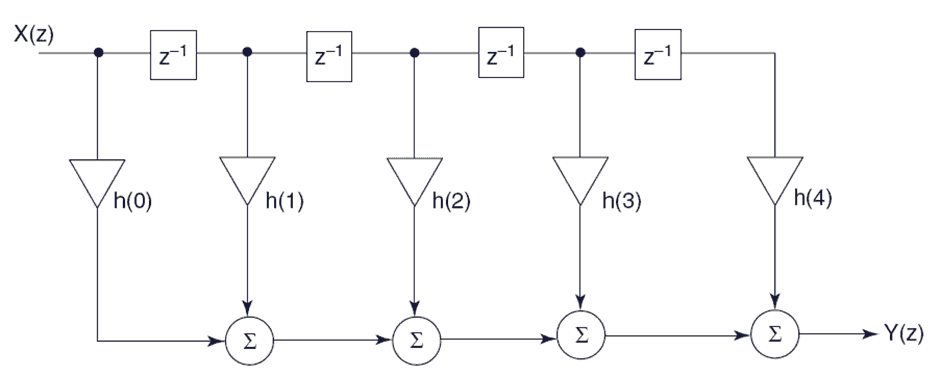
\includegraphics[width=0.75\textwidth]{FIRFilter}
                \caption{FIR Filter \cite{firFilterFig}}
                \label{fig:FIRfilter}
            \end{figure}
            
            \subsubsection{Moving Average}\label{moving average}
            {
                A moving average filter is a special case of a FIR filter. Both filters have a finite impulse response, but while a FIR filter have coefficients based on the filters specifications, a moving average filter uses a sequence of scaled 1s as coefficients. As mentioned the regular FIR filter takes each sample value and multiply it with a coefficient and adds the results. A moving average filter do not multiply anything. Instead it adds all sample values and divide it by the length of the filter. This gives the following formula:
                
                \begin{equation}\label{eq:movAvg}
                    \textit{moving average} = \frac{x[n] + x[n - 1] + ... + x[n - N]}{N + 1}
                \end{equation}
                
                where \textit{N} + 1 is the filter length \cite{movAvgFilter}.
            }
        }
    }
   
    \section{Cloud Services} \label{cloudServices}
    {
        Cloud services can be any service available to the user on the internet from a cloud computing provider. The US National Institute of Standards and Technology defines the three main types of cloud service models like this \cite{cloudComputing}:
        
        \begin{itemize}
            \item Infrastructure as a Service (IaaS) is where you use provided hardware to run your existing applications over the Internet. Only the infrastructure is provided. By this definition, Azure is an example of IaaS.
            \item Platform as a Service (PaaS) is a service where a vendor provides a complete set of tools and environment for developing and running applications. A user needs to use the provided languages and infrastructure.
            \item Software as a Service (Saas) is a complete application or service in the cloud which only requires internet access to use.
        \end{itemize}
    }
    
    \section{Application Programming Interface}
    {
        \Gls{api} is a programming interface that enables communication between computer programs. An \gls{api} defines methods for an application or a library. The purpose of an \gls{api} is to make programs easier to use for people, and to make technology easier available for developers \cite{azurePredictive}.
    }
    
    \section{Data Storage}
    {
        A data storage device in this context is a device consisting of computer components that stores digital data. Companies are commonly connected to a server where they store their data in one or several databases. These databases are structured collections of data. The most used type of database is the relational database which consist of data organised in tables. A \gls{dbms} is an application that interacts with the user. MySQL and Microsoft SQL Server are well-known \gls{dbms}s that allows creation, queries and database administration \cite{databaseSystems}. 
        \par 
        The data in a database can be accessed by requesting information, called querying. A query is written in a query language such as \gls{sql}. A query and data manipulation language used for relational databases \cite{HeadFirstSQL}.
    }
    
    \section{Programming}
    {
        \subsection{Python}\label{pythonTheory}
        {
            Python is a high-level, object-oriented programming language. Python is very popular for Rapid Application Development\footnote{Rapid Application Development focus less on planning and more on developing} because of its built in data structures in combination with dynamic typing and binding. Python have a simple syntax which makes it easier to read and in that way reduces the cost of program maintenance \cite{python}. Python is mainly used to "glue" things together, and because of the many libraries available it can be used in a wide range of applications. One of them is machine learning. 
        }
        
        \subsection{R}\label{Rtheory}
        {
            R is a programming language for statistical computing and graphics. One of the strengths with R programming is that it is easy and fast to produce quality plots as well as statistical computation \cite{rprog}. 
        }
    }
    
    \section{Version Control}
    {
        Version control systems are tools made for software teams to help them keep track of changes in code over time. It keeps track of all modifications in the code so that if a mistake is made, it is easy to go back to an earlier revision. This makes it easier for a developer to fix a mistake without affecting the whole team. When working in teams the members usually work with different parts of the code. These parts needs to be merged together, and that is often where problems occur. Version control systems helps the team discovering what causes the problems \cite{versionControl}. 
    }
}

\newpage
\chapter{Materials and Methods}
{
    \section{Concept Explanation}\label{concept}
    {
        The introduction in section \ref{Introduction} addresses Intelecys goal to develop a cloud-based self-learning predictive maintenance application for the process and manufacturing industry. Such an application should predict failures and detect anomalies. The development platform is preferably in Microsoft Azure. Development in Azure can be done in Microsoft Azure Machine Learning Studio, which support development in Python (section \ref{pythonTheory}) and R (section \ref{Rtheory}).   
        \par  
        Our project aims to explore ideas on how to structure a predictive maintenance application, and research the individual parts of it. This will create a foundation for pre-processing and machine learning.
        \par
        A system for predictive maintenance is complex and include several parts and processes. The basis for such a system is to reduce down-time, costs and probability for disasters and improve quality and efficiency. Such a system must be able to detect anomalies and failures as well as predicting when failure, breakdown or maintenance is due. Our idea for implementing these aspects into one system is illustrated in \figref{processConcept}.
        
        \begin{figure}[H]
            \centering
            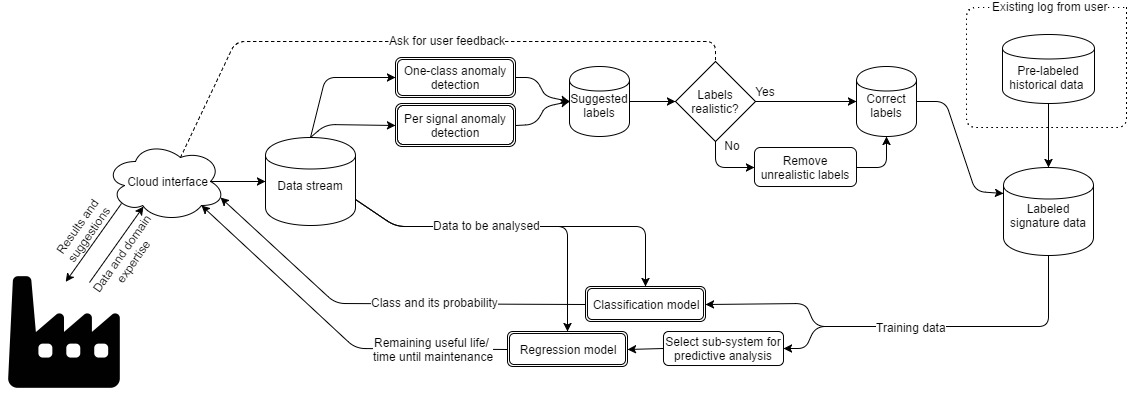
\includegraphics[width=\textwidth]{process}
            \caption{Concept}
            \label{fig:processConcept}
        \end{figure}
        
        The idea is that if historical data has labels for failures, maintenance or other events, it can be used for training a classifier to recognise these events, or even use regression models for predicting when they will occur. In addition, streamed data will be presented to anomaly detection algorithms to determine if a system or signal is out of normal condition. When the system alerts that there is an anomaly in the system, the operator can explore the root-cause of the error, and label the dataset, which later can be used for predicting or classifying. 
        \par
        Since we will do research to create a foundation for developing such a cloud-based self-learning predictive maintenance application for the process and manufacturing industry, it is necessary to explore the individual topics with experiments. We split our idea into 4 parts:
        
        \begin{itemize}
            \item Per signal anomaly detection (Experiment A): Explore methods for detecting anomalies in individual signals. Potential methods are tested on simulated data and signals generated by ourselves to see the anomaly types that are detected. 
            \item Anomaly detection (Experiment B): Explore methods for detecting anomalies on several signals, preferable systems or sub-systems. Potential methods are tested on a simple generated signal, simulator data and real dataset.
            \item Classification of events (Experiment C): Explore methods for using historical faults to detect similar faults in the future. Potential methods for classification are tested on both a simulator dataset and on a real dataset.
            \item Event prediction (Experiment D): Explore methods for predicting when breakdowns or faults will occur, or when maintenance is needed. Potential methods are tested on a dataset with engine breakdowns and one with battery failures.
        \end{itemize}
        
        Additionally, development in Microsoft Azure ML Studio will be compared to development with Python to provide advice in the choice of development platform. A benchmark between these will therefore be performed.
        \par
        The next sections will introduce how the project group is organised, what software is used, which development principles is used and general methods used in several of the experiments.
    }
    
    \section{Project Organising}\label{project organizing}
    {
        The project group is organised with a project manager and a secretary. The project manager keep the position throughout the project, while the secretary position is divided into three periods to even out the workload. The area of responsibility for the project manager is to update project progress in the Gantt-diagram and conduct meetings with the supervisors. The secretary position is responsible for booking room for meetings, summon meetings, write and distribute minutes of meetings and write progress reports before every meeting. Even though the group members has their roles, collaboration and assistance is required to carry out required responsibilities. 
        \par
        During projecting, the thesis problems where defined, and the project group drew a project plan in the form of a Gantt-diagram. The Gantt-diagram was the basis for the every weeks focus and progress, and got dynamically adapted as knowledge, understanding and priorities where made. A meeting was arranged approximately every second week between the project group and the supervisors. In these meetings we discussed the progress in the previous weeks, the expected progress for upcoming weeks and solutions. Every meeting contained of a small demo from the project group to show experiments and potential solutions. In addition to the meeting the project group had continuous communication with Intelecy through chats and telephone conversations. Google's cloud storage service Google Drive has been used for sharing relevant files between the project group and Microsoft SharePoint has been used for sharing files between the project group and Intelecy.  
    }
    
    \section{Software}
    {
        \subsection{Microsoft Azure}\label{microsoft azure}
        {
            Microsoft Azure is a collection of integrated cloud services. Azure offers tools for enterprise, mobile, web and Internet of Things (IoT) among other. Since Azure is a cloud service you can run your apps anywhere as Azure runs on a worldwide network of data centres managed by Microsoft. To protect data on the cloud Microsoft have adopted the new international cloud privacy standard, ISO 27018 \cite{azure}. 
            
            \subsubsection{Machine Learning Studio}\label{AzureMLStudio}
            {
                Microsoft Azure Machine Learning Studio is a cloud service for predictive analytics (see section \ref{predictive analytics}). This makes it possible to create and deploy predictive models that gives analytic solutions. The studio offers a lot of ready-to-use libraries with algorithms that can be used on an internet-connected PC to create and deploy models. Combined with a drag-and-drop interface this gives a predictive solution quickly. As well as having a lot of different built-in packages it also have support for custom code through R or Python scripts. 
                \par
                
                \begin{figure}[H]
                    \centering
                    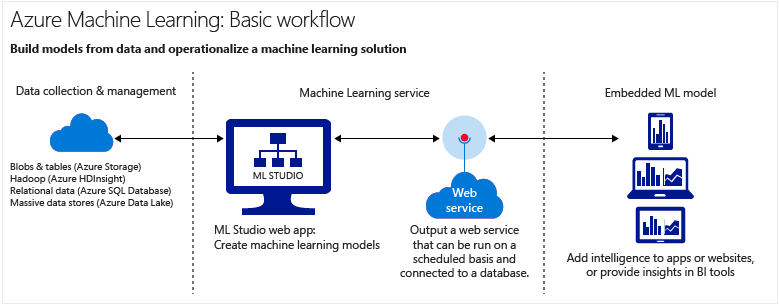
\includegraphics[width=\textwidth]{azureML}
                    \caption{Azure ML - Basic workflow \cite{azureML}}
                    \label{fig:azureML}
                \end{figure}
                
                As seen in \figref{azureML} Azure ML Studio do not only provide the cloud service and predictive analytics model, but also a service that can be used to deploy predictive models as web services (section \ref{cloudServices}) so that the applications can be accessed by others \cite{azureML}. 
                \par
                
                Azure offers several different application programming interfaces (API) for machine learning. One of them is for anomaly detection. The anomaly detection \gls{api} is used to detect different types of anomalous patterns in your data. What this \gls{api} does is that it assigns an anomaly score to each data point that can later be used for generating alerts. As mentioned this is just one of several \gls{api}s offered by Azure \cite{mlAPI}. 
                \par
                
                Building and deploying of a model consists of the following key steps \cite{azurePredictive}:
            
                \begin{itemize}
                    \item Importing raw data
                    \item Data pre-processing
                    \item Feature engineering and data labelling
                    \item Training, scoring and evaluating the model
                    \item Model comparison and selection
                    \item Saving the trained model
                    \item Creating a predictive experiment
                    \item Publishing the web service in Azure Machine Learning
                \end{itemize}
            }
        }
        
        \subsection{Microsoft SQL Server}
        {
            Microsoft SQL Server is a hybrid database platform that have built in security and in-database analytics. It also have an end-to-end mobile BI that transforms data to give insight on any device. Microsoft SQL Server is made for hybrid clouds, which gives an easy mobility to for example Microsoft Azure \cite{aboutMicrosoftSQL}. 
        }
        
        \subsection{Wonderware}
        {
            Wonderware, by Schneider Electric, delivers Human-Machine Interfaces (HMI) to industrial and manufacturing plants. Wonderware delivers their applications across an entire enterprise, including mobile users \cite{aboutWonderware}. 
        }
        
            \subsubsection{Wonderware Historian}
            {
                Wonderware Historian is a large volume plant data historian. It is made to unite a high-speed data acquisition and storage system with a traditional database management system \cite{aboutWonderwareHistorian}. Historian combines advanced data storage and compression techniques with an interface to give an open access to all of your process. Data stored in Historian is easily accessed from your desktop, laptop, tablet or smart phone. Schneider Electric has made a partnership with Microsoft to be able to offer Wonderware Historian Software as a Service (SaaS) (see section \ref{cloudServices}). This is running in the same environment as Microsoft Azure Cloud Services, which is highly secure \cite{wonderwareHistorian}.
            }
            
        \subsection{Share\LaTeX}
        {
            Share\LaTeX is an online, collaborative \LaTeX editor that provides easy collaboration where a team can work together on a single version. Share\LaTeX makes it possible to work from anywhere, both online and offline. Files can be synced through Dropbox and GitHub to make offline work possible. It also keeps track of the document history that tracks all changes done in the document. This let users see what and when something have been changed, as well as giving the option to revert changes if mistakes have been made \cite{sharelatex}. 
        }
    }
    
    \section{Software Development}
    {
        The software and methods used in the project are implemented in Microsoft Azure Machine Learning Studio (see section \ref{AzureMLStudio}), Python or R programming language. The \gls{ml} Studio is used because Intelecy aims to develop a cloud-based service by using Microsoft Azure. Python and R is used for programming since Microsoft Azure supports these scripts in either the \gls{ml} Studio or in their Spark clusters. Python and R are much used languages for data analysis and machine learning \cite{progammingLanguageForML}. Jupyter Notebook and PyCharm IDE was used for developing and testing code in Python.
        \par 
        By developing scripts in one of the mentioned programming languages, these can run either in Azure \gls{ml} studio or in a cluster to process large amounts of data. Both Python and R has a lot of available packages for pre-processing, machine learning and statistical methods. 
        \par
        Experiments and code developed in Microsoft Azure are automatically saved and backed up in Microsoft Azure, at any time previous versions of an experiment can be accessed.

        \subsection{Libraries}\label{Libraries}
        {
            Packages used in Python for the experiments:
            
            \begin{itemize}
                \item NumPy is short for Numerical Python and is a much used library in scientific computing in Python. It provides efficient multidimensional array object, functions for element-wise computation, random number generators, linear algebra function, Fourier transform and much more. In addition, NumPy is used as a container to pass data between algorithms \cite{pythonDA}. 
                \item Pandas is a Python library that provides functions and data types to work with structured data. A DataFrame in pandas provide column-oriented data structures with labels for both columns and rows. The package provides functions with high performance computation for whole tables and columns \cite{pythonDA}.  
                \item SciPy is a collection of Python packages for scientific computing. It consist of methods for signal processing, statistics, linear algebra and much more \cite{pythonDA}.  
                \item Matplotlib is a Python package for producing a wide variety of plots and visualisations. It supports interactivity, which includes a toolbar in plots which enables to pan and zoom in figures \cite{pythonDA}. 
                \item \Gls{skl} is a package which provides functions for data analysis and data mining. Included is functions for pre-processing, machine learning, dimensionality reduction and model selection \cite{pythonML}.
            \end{itemize}    
            
            \par 
            Throughout the project, Python is much used for pre-processing, implementation of statistical reasoning and machine learning models and testing of these models. Pandas and NumPy are used for structuring data and running computational-effective operations on parts of or complete datasets. SciPy is used for signal processing and some statistics. Matplotlib is used to generate plots and visualisations of data to increase knowledge about original data, features, result and so on. \Gls{ml} models and pre-processing techniques has been used from the Scikit-learn package.
            \par
            In addition, R is used for an experiment with per signal anomaly detection. There are a lot of available packages for anomaly detection in R. Twitter's anomaly detection package is the reason for why R is included as a programming language in our project. It includes two functions, one for detecting anomalies in vectors, and for detecting anomalies on time series data. 
        }
    }
    
    \section{Development Principles}
    {
        In this project we will follow some principles from agile software development. Additionally, we chose to practise the relevant phases of the \acrfull{crisp-dm} process for our experiments.

        \subsection{Agile Software Development}\label{agileSoftwareDevlopment}
        {
            Agile software development are well-known principles to follow when developing software. The project group, in collaboration with Intelecy, aims to follow these principles to achieve adaptive planning, continuous feedback and rapid and flexible response to change. The project group values self-organising and motivation in accordance with agile software development principles. The project group work in the same location and will perform pair programming\footnote{Pair programming is an agile software development  technique where two programmers collaborate on the same station. In pair programming there is a driver which write code, and an observer which checks code, these roles get switched frequently.} where it might be useful \cite{whyAgile}.
            \par 
            As mentioned in section \ref{project organizing} meetings will include a demo of the current progress or possible solutions. This is an important principle in agile software development since demos and working software are more informative than documentation alone \cite{whyAgile}. 
            Iterations at two weeks between each demo will help the project group continuous adapt the project plan to maximise the potential result. 
        }
        
        \subsection{CRISP-DM}\label{crisp-dm}
        {
            \Gls{crisp-dm} is a commonly used process for predictive data analytics projects \cite{mlKelleher}. The \gls{crisp-dm} process consists of six key phases as shown in \figref{crisp-dm_fig}. In this project we will not focus on the deployment phase, but the process is still desirable to practise. 
            \par 
            \begin{figure}[H]
                \centering 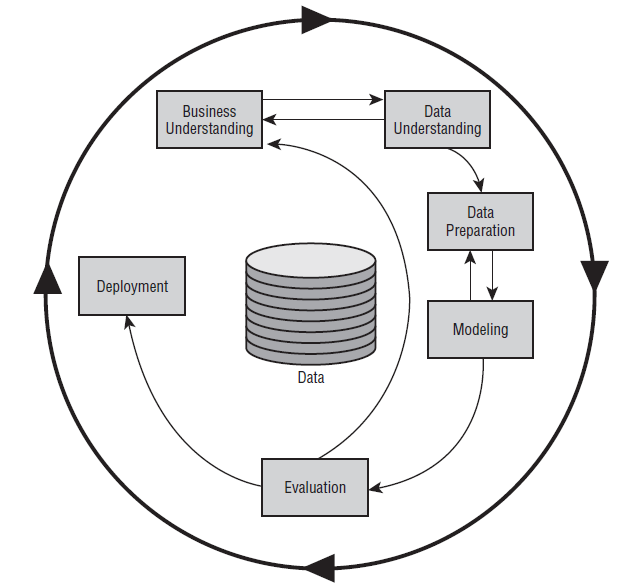
\includegraphics[width=0.6\textwidth]{crisp-dm}
                \caption{CRISP-DM phases and the relationship between them \cite{crisp-dm-Image}}
                \label{fig:crisp-dm_fig}
            \end{figure}
            
            The business understanding phase is about fully understanding the primary goal and its business problem. Predictive data analysis projects never start out with a goal of building a prediction model, but a goal to solve a problem or serve a purpose \cite{mlKelleher}. In this project the project group has focused on understanding the problem and the expected solution.
            \par 
            Second phase of the \gls{crisp-dm} process is data understanding. It aims to fully understand the different data sources available and the types of data in these sources. When a thorough understanding is made the next phase starts which is data preparation.
            \par 
            The data preparation phase aims to take the data from the available sources and structure them into an \gls{abt}. The phase also include handling missing and uncertain data, data transformation and feature extraction to prepare data for the machine learning models, which is the next phase.
            \par 
            Modelling involves building a range of prediction models which will be tested. When the assumed best fit model is chosen, the process goes into the evaluation phase which will ensure that the chosen model is fit for its purpose. Evaluation involves checking that the model will make accurate predictions on new data to make sure that problems like over-fitting and under-fitting is avoided.
            \par 
            The last phase in the \gls{crisp-dm} process as can be seen in \figref{crisp-dm_fig} is deployment. This phase deals with actually deploying the built model to serve its purpose. This includes how the model can maintain its accuracy and be merged into an existing system.

        }
    }
    
    \section{General methods}
    {
        \subsection{Methods for knowledge discovery} \label{knowledge-discovery-methods}
        {
            \subsubsection{Data quality report}\label{dataQualityReport}
                    {
                    A data quality report is a helpful and important tool during a knowledge discovery process. Such a report describes the characteristics of each feature in a dataset. The report is often split into continuous and categorical features and shows measures of central tendency and variation. Continuous features contained in the quality report can be described with feature name, count, missing values ratio, minimum, maximum, standard deviation, variation and more. While categorical features include feature name, count, missing values, most frequent category and the frequency of that category, the second most frequent category and so on \cite{mlKelleher}.
                    \par
                    A dataframe in the pandas package in Python has a built-in function for quality reports which gives a good selection of information for each feature \cite{pythonDA}. Additionally, we created our own function for quality reports that provides the necessary description and some flexibility. The function is shown in the code snippet in \figref{DataQualityReportCode}.
                    
                    \begin{figure}[H]
                        \centering \RecustomVerbatimEnvironment{Verbatim}{BVerbatim}{} \inputminted{python}{thesis/Code/DataQualityReport.py}
                        \caption{Data quality report function}
                        \label{fig:DataQualityReportCode}
                    \end{figure}
            }
            
            \subsubsection{Distribution evaluation - Histogram plot}
            {
                Histograms of the individual sensors are normally included in a data quality report. These can teach us about the distributions of the sensor values and thereby help us evaluate features \cite{mlKelleher}. To simplify the process of creating histograms from sensors, we have created an adaptable function to visualise the histograms in a readable manner. The function is shown in \figref{histogramCode}.
                
                \begin{figure}[H]
                    \centering \RecustomVerbatimEnvironment{Verbatim}{BVerbatim}{} \inputminted{python}{thesis/Code/histogramCode.py}
                    \caption{Code for generating histograms}
                    \label{fig:histogramCode}
                \end{figure}
                
            }
        
            \subsubsection{Normalisation}
            {
                As mentioned in section \ref{data-transformation-theory}, normalisation is to transform the data from one range to a new specific range. The formula for standard normalisation in the range 0 to 1 is:
                
                \begin{equation}
                    \label{normalisation-eq}
                    \text{Normalised} = \frac{X_i-X_{min}}{X_{max}-X_{min}}
                \end{equation}
                    
                To normalise into a different range than 0 to 1 we scale the normalised value by this formula:
                
                \begin{equation}
                    \label{scaling-eq}
                    \text{Scaled} = \text{Normalised} \times (R_{max}-R_{min}) + R_{min}
                \end{equation}
                    
                Where $R_{max}$ is the upper bound and $R_{min}$ is the lower bound of the range.
                \par
                If the range of the raw data is not predefined the normalisation is done by first finding the max and min values of each feature in a training dataset and use these values to normalise the training set and test set.
            }
            
            \subsubsection{Missing data}\label{missingData}
            {
                Section \ref{pre-processing-theory} mentions that real world datasets can contain missing values. The missing values can not be used in the \gls{ml} algorithms, but they can represent valuable information. Therefore methods for handling the missing values need to be applied.
                \par
                If the data are logged in delta, where only changes are recorded and all other data points are missing, the missing data can be replaced with the last known value. This is also known as forward-fill. An example of delta logging and forward filling of binary values is shown in \figref{deltaLogging}.
                \begin{figure}[H]
                    \centering 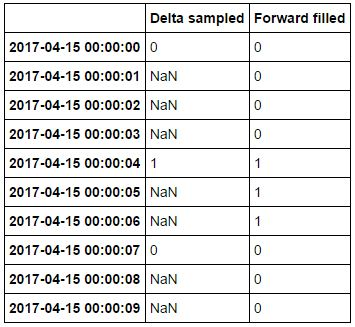
\includegraphics[width=0.5\textwidth]{deltaLogging}
                    \caption{Delta sampling and forward filling of binary signals}
                    \label{fig:deltaLogging}
                \end{figure}
                \par                
                In another case where we do not have delta logging, but continuous logging, the missing values can be handled by deleting the whole row. Another method is imputation. This method replaces the missing value with a plausible estimated value. The mean or median of the feature is most commonly used for continuous logging, but other values, such as 0 can be used in some cases. \cite{mlKelleher}.
                \par
                In cases were the data is logged irregular, some knowledge of the data needs to be gathered before a decision on what to do with the missing data can be made. For instance if a feature only contains one value besides the missing values, the missing values can be replaced with this value. Another approach can be to look at the rows in the dataset, and if the row contains more than a given number of missing values the entire row can be eliminated from the dataset. The same approach can be used on the columns \cite{supervisedMLsecom}.
            }
            
            \subsubsection{Moving Window Functions}\label{movingWindow}
            {
                In time series data, it is possible to transform the data using statistics, evaluated over a moving window. 
                Mean is one of the operations that can be applied in the window. The window is moved through the data, one sample at a time. Moving window functions like these, can be done for any suitable function, such as median, difference, variance, kurtosis\footnote{In statistics, kurtosis is a measure of pointedness in the shape of a distribution} and skewness\footnote{In statistics, skewness is a measure of the asymmetry of a distribution} \cite{pythonDA}.
                \par 
                In Python, we calculate moving window functions from time series data, by using a built-in function in the pandas package (section \ref{Libraries}). An example is shown in \figref{RollingImpl} 
                
                \begin{figure}[H]
                    \centering \RecustomVerbatimEnvironment{Verbatim}{BVerbatim}{} \inputminted{python}{thesis/Code/Rolling.py}
                    \caption{Moving window function implemantion in Python}
                    \label{fig:RollingImpl}
                \end{figure}
                
                The method above, can also be used to implement the moving average filter, mentioned in section \ref{moving average}.
            }
            
            \subsubsection{Detrend}\label{detrend}
            {
                Detrending is a statistical method that can be implemented to remove a trend from a time series signal. 
                A trend can be that the mean changes over time, and can therefore hide sub-trends. The idea is that a trend in a signal can cause an distortion that hides underlying sub-trends or anomalies.
                \par 
                It is possible to remove trend from both linear, exponential and even cyclic signals. For a linear trend the least squares linear regression line for the signal is fitted, and the deviation from this line can be subtracted from the signal \cite{detrend-web}.
                \par
                In Python, the SciPy package explained in section \ref{Libraries}, has a signal module that can use a detrend function, which simply removes a possible linear trend along an axis in the provided data \cite{pythonDA}.
            }
        }
        
        \subsection{Methods for Machine Learning}
        {
            \subsubsection{Hyperparameter optimisation}\label{HyperparameterOptimisation}
            {
                In the topic of \gls{ml}, two types of parameters exists. One type of parameter is learned during training (e.g weights in an \gls{ann}), the other type is the parameters or settings of the algorithm (e.g type of activation function in an \gls{ann} or number of neighbours in \gls{knn}) \cite{pythonML}. The settings of an algorithm do not get updated during training and must be manually chosen or optimised. Optimising these settings parameters is referred to as hyperparameter optimisation, which has different techniques for choosing the best performing parameters. Grid search is one of these techniques, and aims to find the optimal combination from a given set of hyperparameter values.
                \par
                Grid search is a brute-force exhaustive search for an optimal set of hyperparameters from a given set of values for different hyperparameters. It evaluates every possible combination of these parameter values and can return the best performing algorithms and its settings \cite{pythonML}. 
                In Python, the grid search algorithm can be implemented by using the grid search model in the \gls{skl} package, described in section \ref{Libraries}. An example of such a grid search implementation can be seen in the code snippet in \figref{gridSearchExample}.
            
                \begin{figure}[H]
                    \centering                    \RecustomVerbatimEnvironment{Verbatim}{BVerbatim}{} \inputminted{python}{thesis/Code/GridSearch.py}
                    \caption{Hyperparameter optimisation - Grid search example}
                    \label{fig:gridSearchExample}
                \end{figure}
            }
            
            \subsubsection{Machine Learning Implementation} \label{mlImpl}
            {
                Machine learning models will be implemented in Python by using the available models in the \gls{skl} package (section \ref{Libraries}). The package contain several types of supervised \gls{ml} models, such as linear models, \gls{svm}s, \gls{nn}, ensemble models and several more. The supervised learning models has the same implementation. \Figref{supLearnModels} illustrates this, by using \gls{mlp} as an example.
                
                \begin{figure}[H]
                    \centering                    \RecustomVerbatimEnvironment{Verbatim}{BVerbatim}{} \inputminted{python}{thesis/Code/MLmodels.py}
                    \caption{Implementation of supervised learning models in Python }
                    \label{fig:supLearnModels}
                \end{figure}
                
                \par 
                The unsupervised learning models implementation is similar, but target data is not applied to the model. \Figref{unsupLearnModels} shows an example of implementation, using K-means clustering (section \ref{K-MeansClusteringTheory}). 
                
                \begin{figure}[H]
                    \centering                    \RecustomVerbatimEnvironment{Verbatim}{BVerbatim}{} \inputminted{python}{thesis/Code/UnsupModels.py}
                    \caption{Implementation of unsupervised learning models in Python }
                    \label{fig:unsupLearnModels}
                \end{figure}
            }
        }
        
        \subsection{Methods for scoring}\label{methods-for-scoring}
        {
            Scoring can be done in a number of ways, depending on the type of problem (section \ref{scoringMethods}). Kelleher has in his book explained several of these scoring methods for both classification and regression \cite{mlKelleher}.
        
            \subsubsection{Classification scoring}
            {
                The accuracy measure is as mentioned in section \ref{scoringMethods} an often used measure for scoring classifications. 
                
                \begin{equation} \label{accuracy}
                    \text{Classification accuracy} = \frac{TP+TN}{TP+TN+FP+FN}
                \end{equation}
                    
                Recall is the true positive rate (TPR) and is also called sensitivity. This is the probability that positive predictions are correctly classified:
                
                \begin{equation}
                    Recall = \frac{TP}{TP+FN}
                \end{equation}
                    
                Precision is the proportion of positive predictions that are correctly predicted: 
                
                \begin{equation}
                    Precision = \frac{TP}{TP+FP}
                \end{equation}
                    
                $F_1$ measure is a single performance measure that calculate the harmonic mean of precision and recall:
                
                \begin{equation}
                    \text{$F_1$ measure} = 2\times \frac{precision \times recall}{precision+recall}
                \end{equation}
                
                All the above formulas are based on the confusion matrix, and are used for scoring classifications.
            }
                
            \subsubsection{Regression scoring}
            {
                As mentioned in section \ref{scoringMethods} scoring of a regression model can be done by calculating the \gls{mse}:
                
                \begin{equation}\label{mse-eq}
                    \text{MSE} = \frac{1}{n} \sum_{i=1}^{n} (Y_{i}-\hat{Y}_{i})^{2} 
                \end{equation}
                
                The \gls{mse} is in some cases a good function to use for optimising predictions since it emphasises large error. The problem on the other hand is that it does not give a lot of sense. Therefore, the \gls{mae} can give an indication of how large the average prediction error is. \Gls{mae} is the average of the absolute error of all predictions, and is given by:
                
                \begin{equation}\label{mae-eq}
                    \text{MAE} = \frac{1}{n} \sum_{i=1}^{n} \abs{Y_{i}-\hat{Y}_{i}}, 
                \end{equation}
            }
        }
    }
    
    \section{Data}
    {
        The first part of the project, all data were collected from a simulator made in Wonderware by Intelecy (section \ref{simulator}). As mentioned in section \ref{problem}, real, historical data were promised, but not obtained, thus new datasets needed to be explored. By doing research on publicly available datasets and by generating a dataset ourselves we ended up with using these datasets:
        \begin{itemize}
            \item \textbf{Time series anomaly detection dataset:} Used for per signal anomaly detection (experiment A). The dataset is generated by us.
            \item \textbf{Simulator:} Used for per signal anomaly detection, anomaly detection and classification (experiment A-C).
            \item \textbf{Semiconductor Manufacturing (SECOM):} Used for both anomaly detection (experiment B) and classification (experiment C).
            \item \textbf{NASA - Turbofan Engine Degradation Simulation Dataset:} Used for event prediction (experiment D).
            \item \textbf{Battery dataset:} Used for event prediction (experiment D).
        \end{itemize}
        
        \subsection{Time series anomaly detection dataset}\label{timeSeriesData}
        {
            Time series anomaly detection (section \ref{anomalyDetection}) on individual parameters can be valuable in root-cause analysis or for detecting anomalies on vital parts of a system. To be able to explore which anomalies the different time series anomaly detection algorithms can detect, we chose to make a small dataset with different kinds of anomalies. In the upcoming figures the created anomalies is marked by a Navajo white colour. 
            \par
            The first signal is a periodical signal as described in section \ref{anomTimeTypes}. It is built up by sine waves with uniform noise and 6 periods with anomalies, as marked in \figref{AnomType1}. The first anomaly illustrates too early fall, while the second is a too early growth. The next three anomalies are single point outliers and the last illustrates a breakdown. All these are contextual anomalies (section \ref{anomDefinitions}).
            
            \begin{figure}[H]
                \centering
                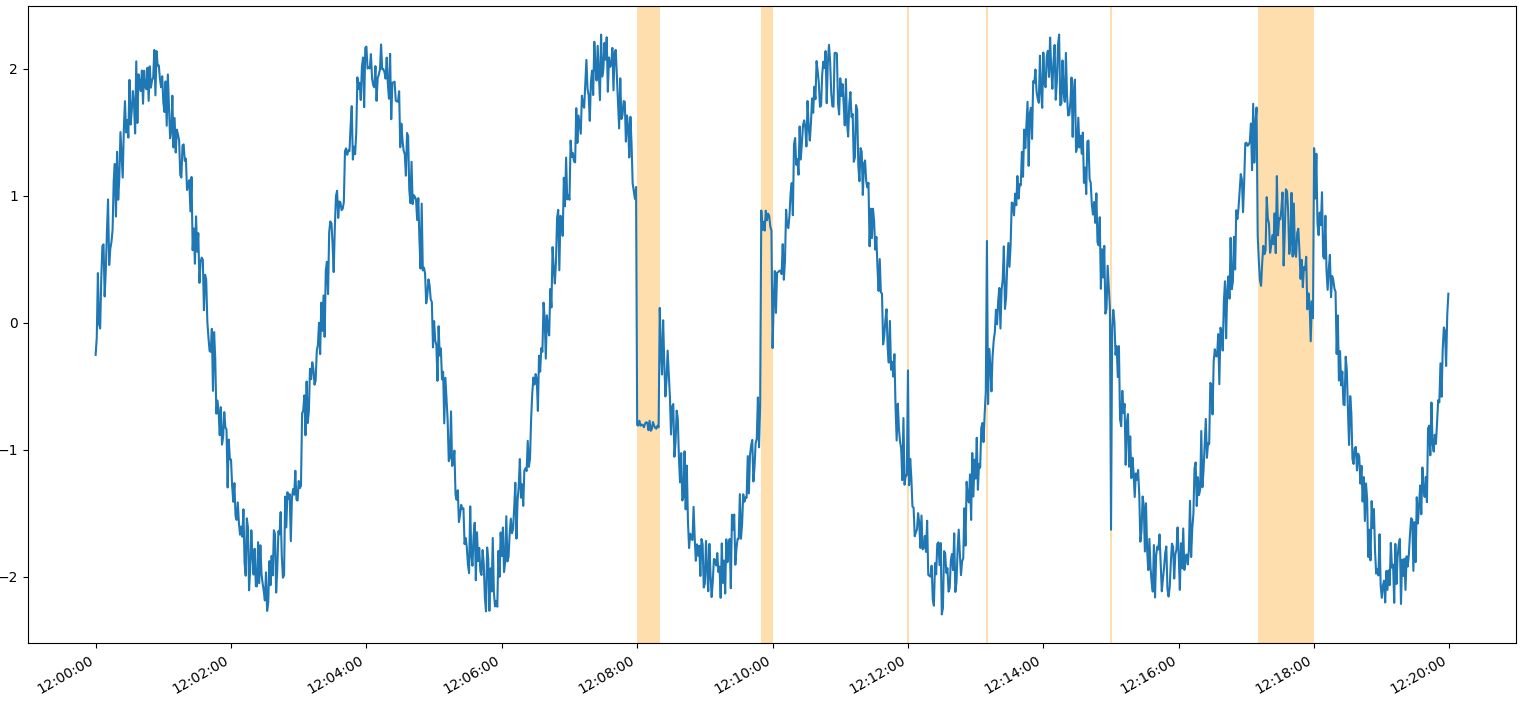
\includegraphics[width=0.9\textwidth]{AnomType1}
                \caption{Test signal with sudden fall and growth, random peaks and breakdown indication}
                \label{fig:AnomType1}
            \end{figure}
    
            \Figref{AnomType2} shows the second signal, which has the same base signal, but the anomalies are changed. Anomaly number one indicates increasing noise, and number two has a steeper and higher peak than usual. The first period of anomalies contains both point and contextual anomalies (section \ref{anomDefinitions}), while the second period mostly consist of point anomalies.
            
            \begin{figure}[H]
                \centering
                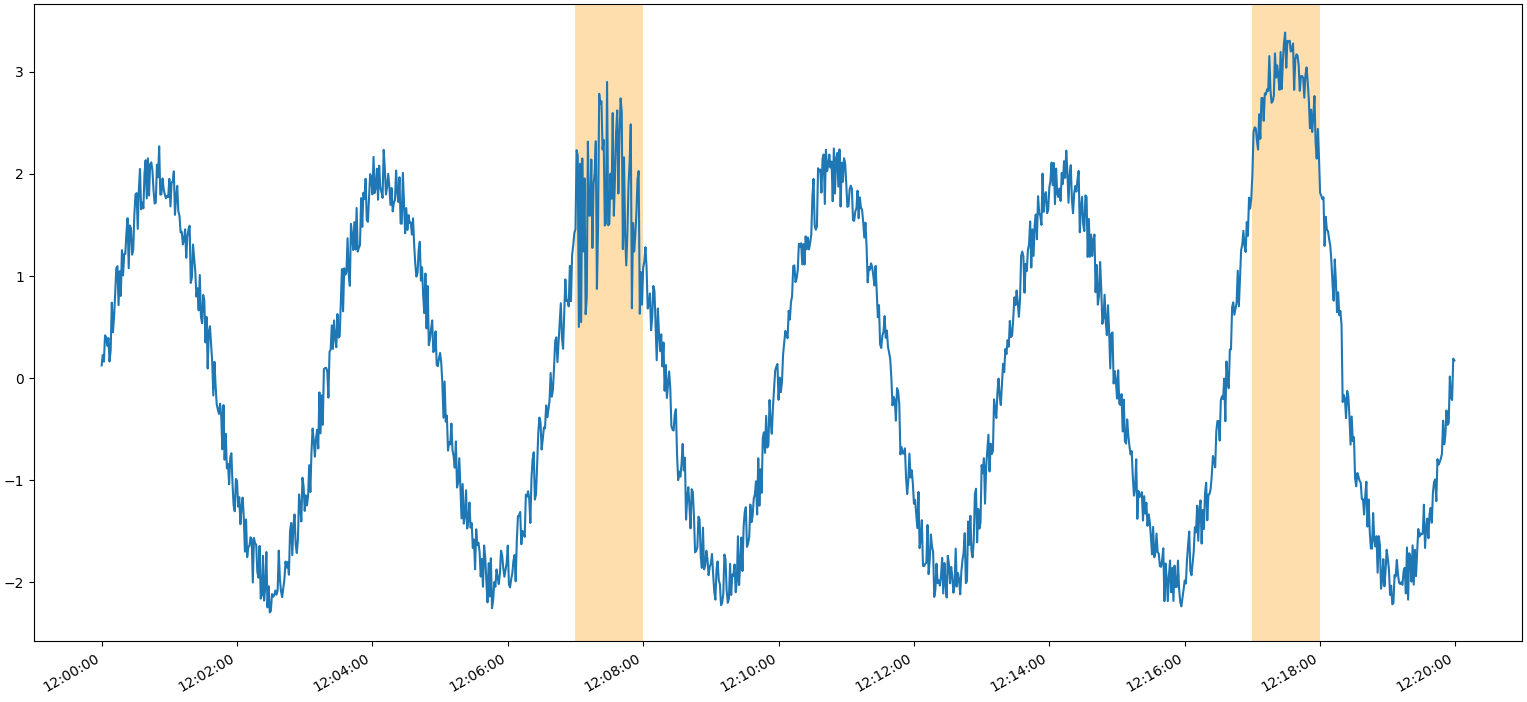
\includegraphics[width=0.9\textwidth]{AnomType2}
                \caption{Test signal with added noise on one peak, and added growth on another}
                \label{fig:AnomType2}
            \end{figure}
            
            The third signal has the same sine wave as a base, but without noise. Three periods with noise are added to the signal, which is one type of anomalies in this signal. These are also contextual, but will indicate if we can detect increasing noise. Another type of anomaly in the signal is that the last peak holds the top value, and illustrates a signal lasting longer than expected. It is of the time series anomaly type illustraded in \figref{timeSeriesAD} in section \ref{anomalyDetectionTimeSeries}. \Figref{AnomType3} shows the described signal.
            
            \begin{figure}[H]
                \centering
                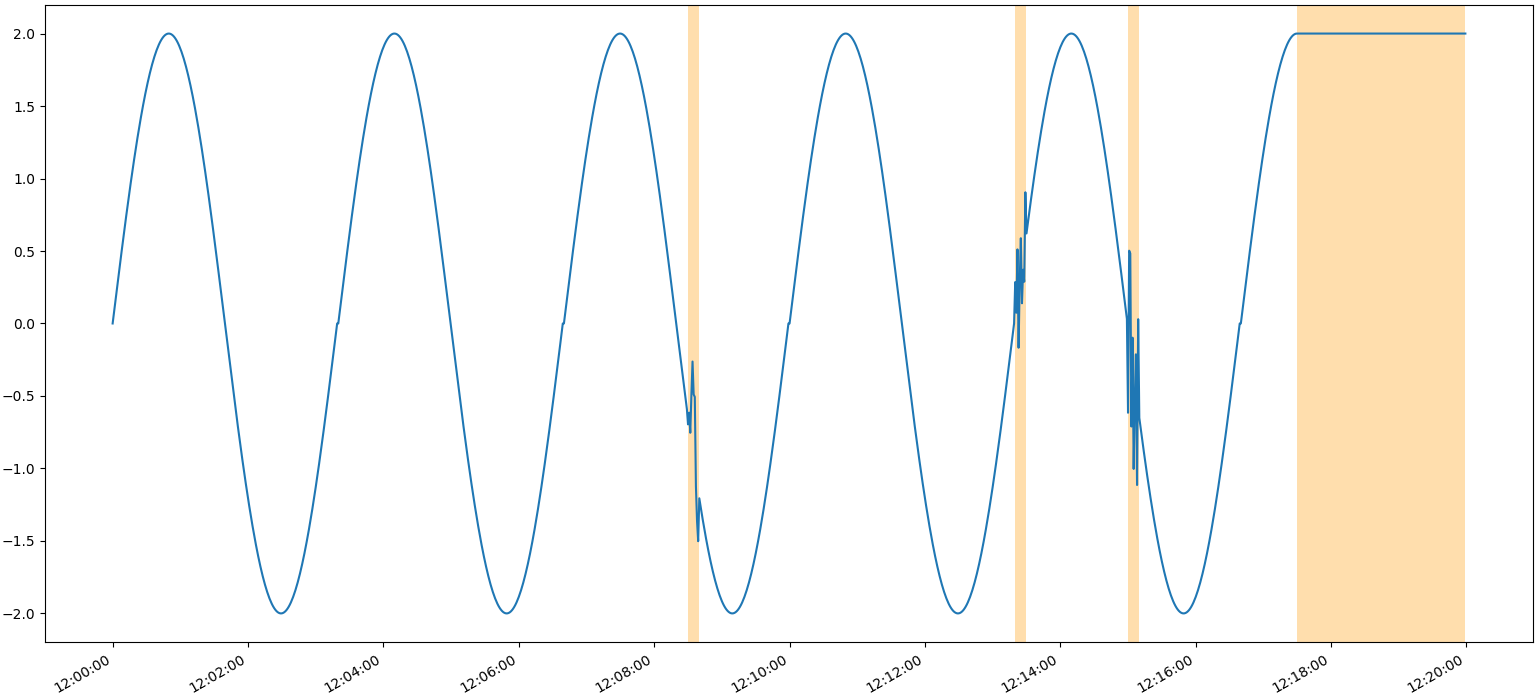
\includegraphics[width=0.9\textwidth]{AnomType3}
                \caption{Test signal with noise as anomalies, last peak value held to illustrate time dependent anomaly}
                \label{fig:AnomType3}
            \end{figure}
            
            The last signal consists of a linear signal with noise since a known challenge for time series anomaly detection algorithms is to be able to detect anomalies in signals that grow or fall over time. The two first anomalies indicated in \figref{AnomType4} are higher values than normal, while the last anomaly consists of an increment of slope. 
            
            \begin{figure}[H]
                \centering
                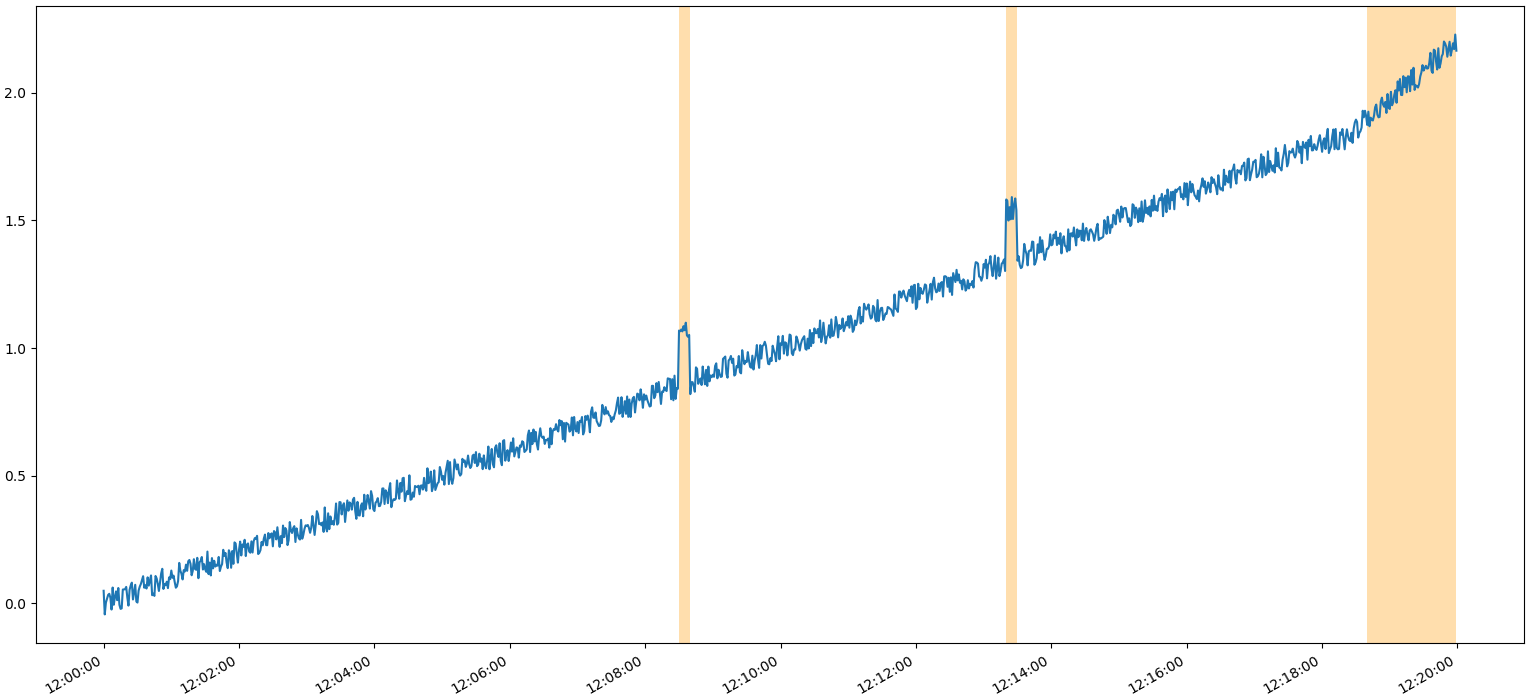
\includegraphics[width=0.9\textwidth]{AnomType4}
                \caption{Test signal with linear increasing slope with two sudden growths and rapid increasing values at the end}
                \label{fig:AnomType4}
            \end{figure}
        }
        
        \subsection{Simulator} \label{simulator}
        {
            The simulator runs continuous in automatic mode, with the possibility to turn into manual mode to manipulate signals and generate anomalies and alarms. The simulator can be accessed through Wonderware WindowViewer, where the process can be monitored or controlled. Alarms, signals and settings are stored and logged in Wonderware Historian, which is accessed through a Microsoft SQL Server.
            
            \begin{figure}[H]
                \centering 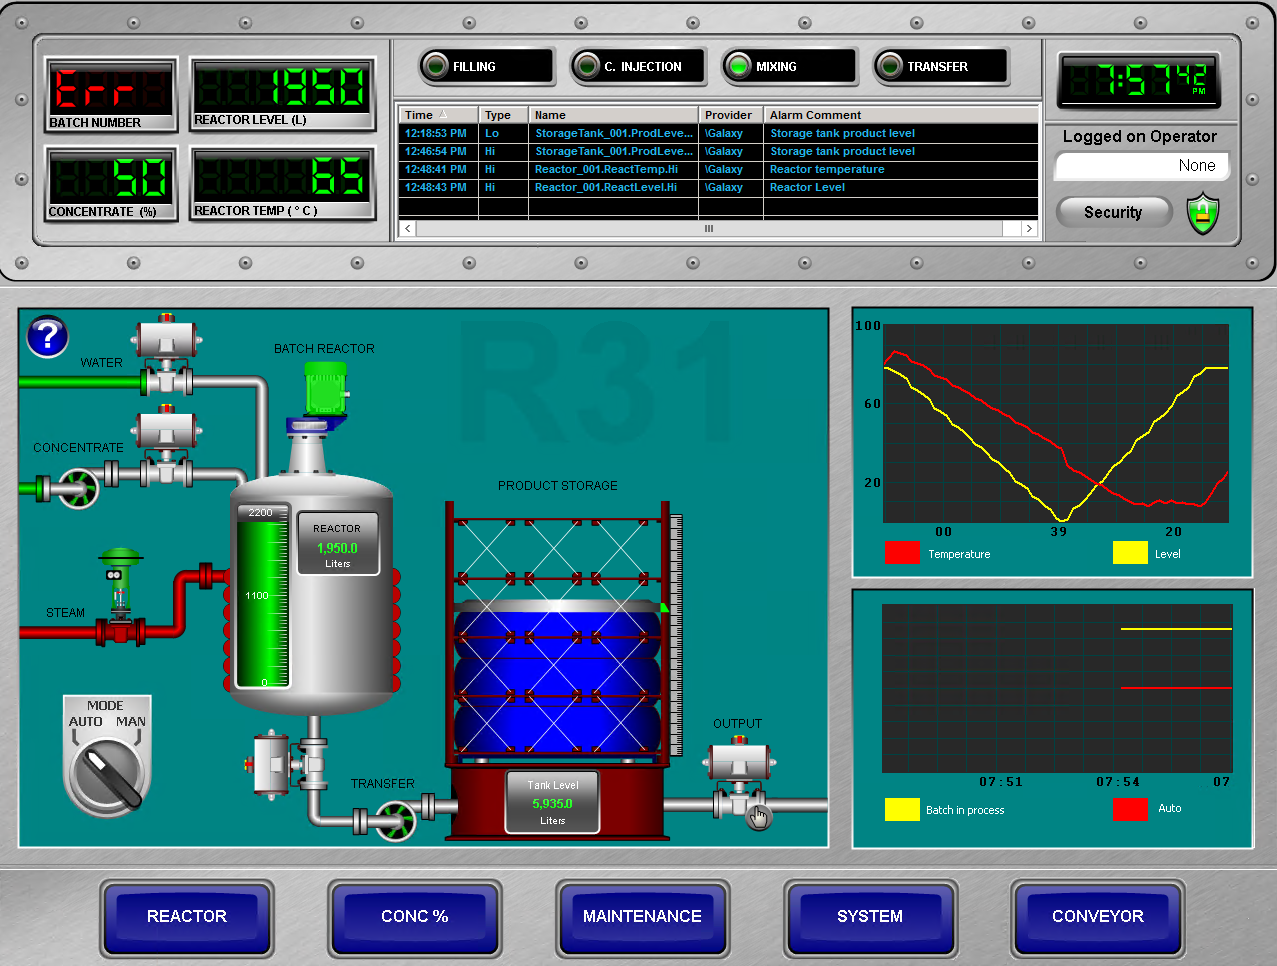
\includegraphics[width=1\textwidth]{Simulator}
                \caption{Simulator view from Wonderware WindowViewer}
                \label{fig:simulator_fig}
            \end{figure}
            
            \par
            \Figref{simulator_fig} shows a section of the simulator and its process. The simulator consist of several reactors as the one showed in the figure, but only one of them has a graphical user interface. The process that is simulated is a production of a mixture that needs to have a certain concentrate and temperature before it is transported to product storage. The reactor has a water inlet with a valve, a transfer pump and valve for the concentrate and a steam valve. A batch is made by first filling water and concentrate to the right proportion of mixture. Secondly the batch gets heated up to a desired temperature, while the batch reactor mixes the liquids. When the temperature reach the requirement the batch gets transferred to the product storage. When the product storage is full the product is further transferred. 
            \par 
            Temperature, level in reactor and storage, mode and the state of valves and pumps is logged in one database, and alarms in another. Logging is done in delta, which means that a value is logged only when changed, as shown in \figref{deltaLogging}. Each logged row consist of a lot of data, one logged instance of temperature has a lot of data, but the columns of most importance are: DateTime, TagName, Value, OPCQuality, wwRetrievalMode and wwTimeZone. \Figref{simulator_history_data} display a small extraction from the logged simulator data from Wonderware Historian.
            
            \begin{figure}[H]
                \centering 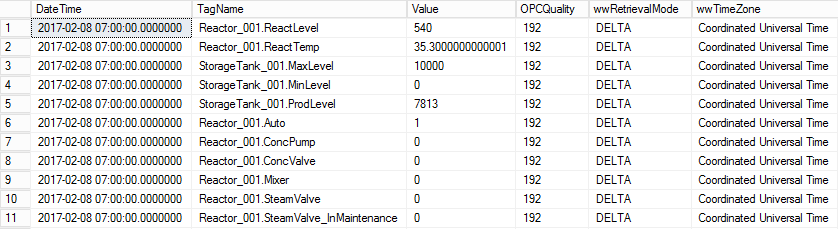
\includegraphics[width=0.9\textwidth]{SimulatorData1}
                \caption{Small extraction of logged simulator data from Wonderware Historian}
                \label{fig:simulator_history_data}
            \end{figure}
            
            \Figref{simulator_plot_norm} shows a plot of the normal state of most of the simulator signals. 
            
            \begin{figure}[H]
                \centering 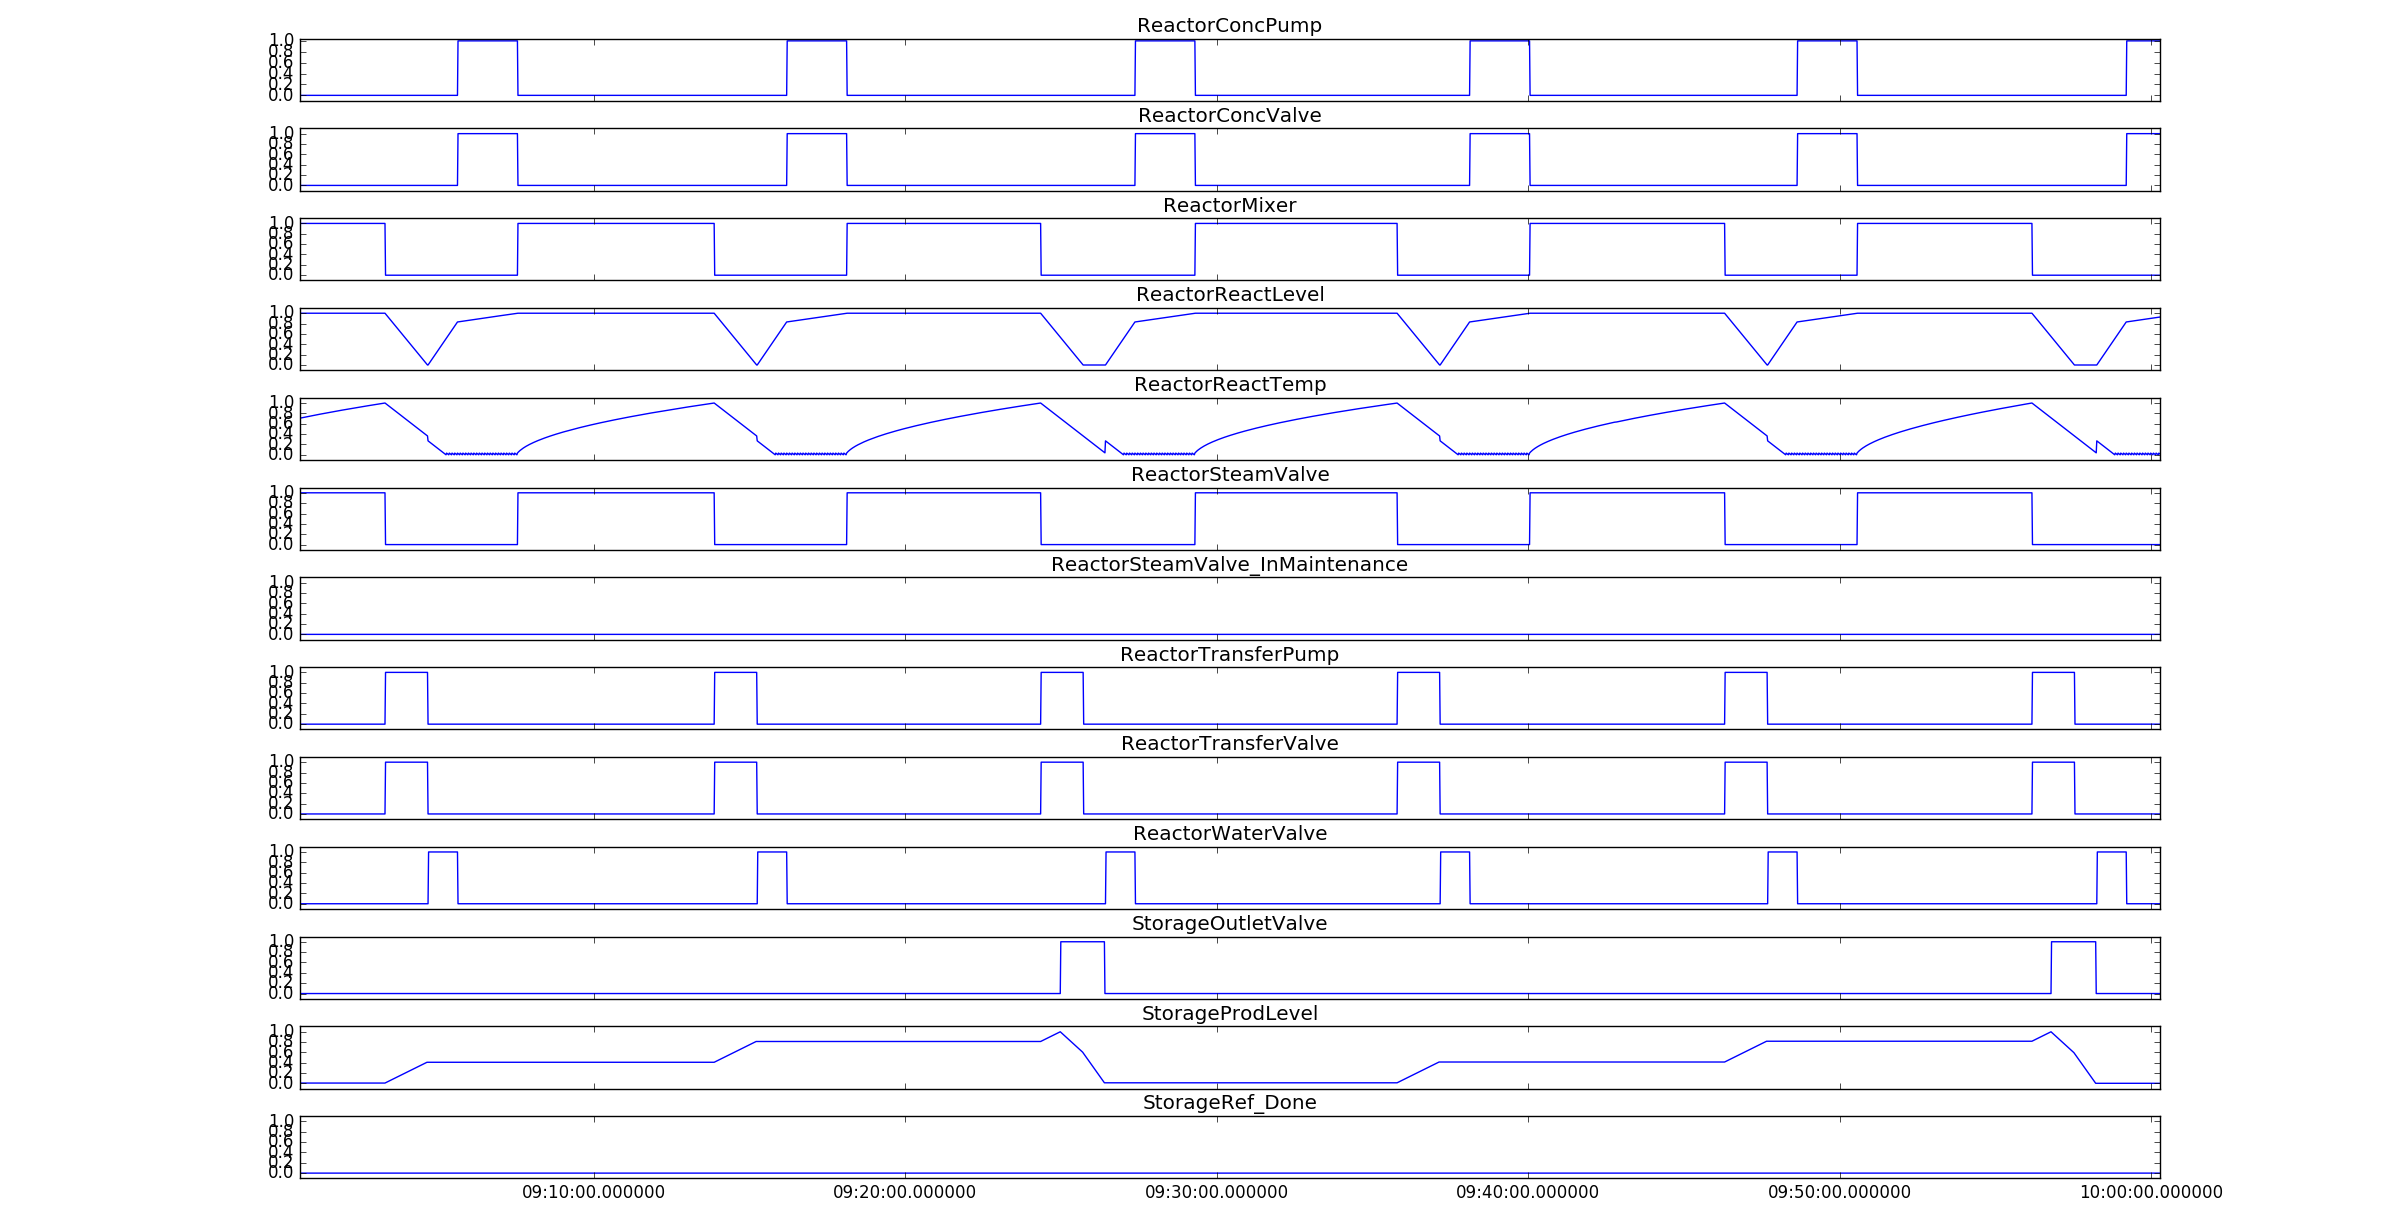
\includegraphics[width=\textwidth]{NormalSimData}
                \caption{Plot of normal data from simulator}
                \label{fig:simulator_plot_norm}
            \end{figure}
            
            \par 
            As mentioned, alarms get logged in a separate database. Each row in the database corresponds to an alarm, and consist of a lot of columns. The columns of most importance is: AlarmID, TagName, AlarmClass, AlarmType, Priority, Limit, AlarmValue, OriginationTime and OriginationTimeZoneOffset. 
            \par
            The data available from the simulator is generated from the simulator and is therefore not effected by physics and other influences a real world process would. The result of this is that data and trends are continuous and have little variance. As an example, the temperature increases with a constant slope as long as the steam valve is open. When the steam value is closed the temperature instantly stops to increase and start decreasing.  
        }
        
        \subsection{Semiconductor Manufacturing (SECOM)} \label{secomData}
        {
            The lack of physical dependencies in the simulated data causes few complex patterns, which in turn eliminates the need for \gls{ml}. Therefore the \gls{secom} dataset was introduced. It contains real data from an industrial semiconductor manufacturing plant. The dataset was donated for \gls{ml} purposes in 2008, and is publicly available from the UCI Machine Learning Repository.
            \par
            The dataset contains 591 features, 1567 samples of which 104 are labelled as outliers, hence has class imbalance. The classes imply a pass or fail of a product, where -1 corresponds to pass and 1 corresponds to fail. As with any real life data situations this data contains null values varying in intensity depending on the individual features. This needs to be taken into consideration when investigating the data either through pre-processing or within the technique applied\cite{uciML}.
            \par
            The dataset has timestamps for each sample, but they have no fixed frequency, thus it is not a time series. Other than that, there is no description of the features, and no indication of sensor types, which draws us back to the idea that an algorithm should be adaptable to the data, hence a data-driven approach.
            \par
            The \gls{secom} dataset is also known to be a challenge to classify \cite{supervisedMLsecom}, and a plot of 3 component PCA, as shown in \figref{secom-PCA-plot}, illustrates this. The plot shows that the classes are evenly distributed.
            \begin{figure}[H]
                \centering
                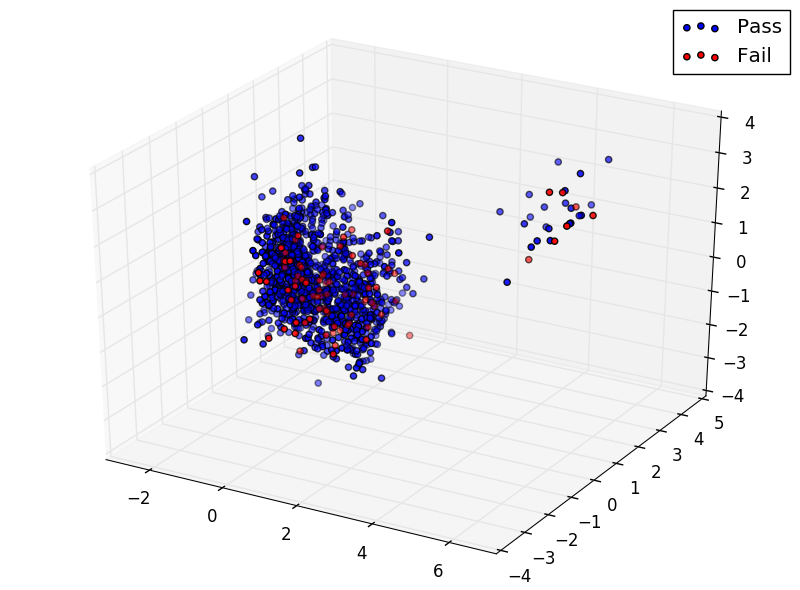
\includegraphics[width = 0.9\textwidth]{SECOM_PCA_3_plot}
                \caption{SECOM dataset reduced to 3 components with PCA}
                \label{fig:secom-PCA-plot}
            \end{figure}
        }
    
        \subsection{NASA - Turbofan Engine Degradation Simulation Dataset}\label{nasaData}
        {
            The data collected from the simulator is not suitable for prediction of time until an event. Therefore a dataset from NASA was introduced, and it is applicable for predicting time until an event (maintenance, failure etc.), and in this case prediction of \gls{rul} is the target. The NASA dataset was made available for public use at the International Conference on Prognostics and Health Management (PHM08) \cite{nasadata}. PHM08 released a competition on the dataset in 2008, where the goal was to achieve the best prediction of \gls{rul}.
            \par
            The NASA datasets are multiple variable time series data representing simulated turbofan engines degradation. Three datasets are available: training, testing and validation set. The training set consists of 218 unspecified units and their measurements, from working order, until the units break down. The testing and validation set has the same parameters, but in difference to the training set the datasets stops some random time prior to complete failure. 
            \par
            Each unit has 26 different parameters logged for each cycle including 21 sensor values, 3 operational settings, engine number and cycle number. The operational settings and sensor values have no description or unit. It is given that the three operational settings have a considerable effect on engine performance and that both the operational settings and the sensor values are contaminated with sensor noise. 
            \par
            As mentioned the dataset is of unspecified units, all the information given is that the units are turbofan engines, with no specifications of type or operational modes. It is given that each engine starts with different degrees of initial wear or manufacturing variation which is unknown, but considered as normal. Time series data is logged as cycles, and the length of each run varies between 128 and 356 cycles. Statistics of the run length are shown in table \ref{nasaRunLength}.
            
            \begin{table}[H]
                \centering
                \begin{tabular}{|l|l|}
                    \hline
                    \textbf{Statistic} & \multicolumn{1}{l|}{\textbf{Run Length}} \\ \hline
                    Minimum            & \multicolumn{1}{c|}{128}    \\ \hline
                    Maximum            & \multicolumn{1}{c|}{356}    \\ \hline
                    Average            & \multicolumn{1}{c|}{210,6}  \\ \hline
                \end{tabular}
                \caption{Run length statistics of units in NASA dataset}
                \label{nasaRunLength}
            \end{table}
            \par   
        }
    
        \subsection{Battery dataset - Li-ion batteries}\label{batteryDataset}
        {
            Similar to the turbofan engine degradation simulation dataset described in section \ref{nasaData}, the battery dataset is provided by Prognostics CoE at NASA Ames, and is available in the NASA Prognostics Data Repository \cite{nasaBatteryData}. The dataset consist of experiments on Li-ion batteries during different conditions for charging and discharging. Impedance measures are included as a damage criterion. The dataset consists of 9 different battery types tested in different conditions, each type and condition has 4 available batteries from initial charge sequence until \gls{eol}. It can be used for predicting remaining charge during discharge cycles or predicting \gls{rul} \cite{nasaBatteryPrognostics}. As mentioned only 4 batteries are available for each battery type, thus it can be challenging to explore this problem with a data-driven approach.
            \par
            The data are achieved through a laboratory setup where Li-ion cells are charged and discharged with different loads and environmental conditions. Periodically measurements are taken to monitor the internal condition of the battery by measuring current in sense branch and battery branch, ratio of the mentioned currents, battery impedance, estimated electrolyte resistance and charge transfer resistance. The charge cycles contains measures of battery terminal voltage, output current, battery temperature, current measured at charger, voltage measured at charger and timestamps, while the discharge cycles contains battery terminal voltage, output current, battery temperature, current and voltage measured at load, timestamps and battery capacity for discharge. The experiment aimed to generate a dataset for determining the health states and predicting end-of-life and end-of-charge for the different batteries \cite{nasaBatteryPrognostics}. 
            \par 
            The dataset is provided in a mat-format, with the structure given in \figref{BatteryDatasetStructure} for each battery.
            
            \begin{figure}[H]
                \centering
                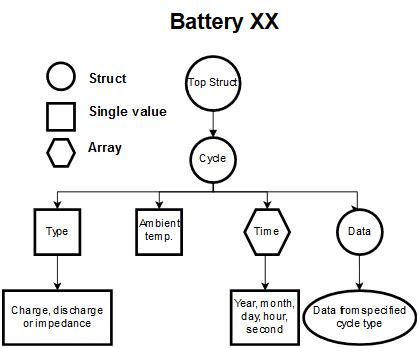
\includegraphics[width=0.6\textwidth]{BatteryDatasetStructure}
                \caption{Battery dataset structure}
                \label{fig:BatteryDatasetStructure}
            \end{figure}
        
            Every type (charge, discharge and impedance) have different measures throughout each cycle. \Figref{BatteryTypeStructure} shows the data attended with each cycle type.
            
            \begin{figure}[H]
                \centering 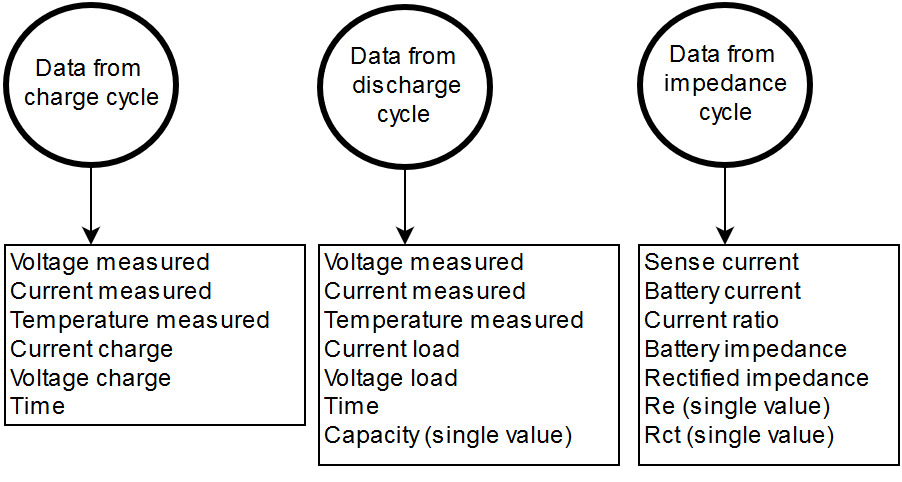
\includegraphics[width=0.6\textwidth]{BatteryTypeStructure}
                \caption{Measurements for each type of cycle during the battery experiment}
                \label{fig:BatteryTypeStructure}
            \end{figure}
            
            For this experiment we will use the batteries of type: FY08Q4, which is labelled as B0005, B0006, B0007 and B0018. The experiment was carried out with an ambient temperature of 24 degrees. Charging was carried out with constant current at 1.5 A, until the battery voltage reached 4.2V and continued in a constant voltage until the charge current dropped to 20 mA. The discharge cycle carried out with a constant current load at 2A until the voltage dropped to about 2.5 V. The experiment continued until the batteries reached \gls{eol} criteria, which is a drop of capacity from 2 Ahr to 1.4 Ahr \cite{nasaBatteryPrognostics}. 
        }
    }
    
    \section{Experiment A: Per signal anomaly detection} \label{prSignalAD}
    {
        This section will focus on the different methods we are trying out for detecting anomalies in individual signal. This includes already existing modules in Microsoft Azure Machine Learning Studio and R.
        
        \subsection{Time Series Anomaly Detection with Azure} \label{timeSeriesAD}
        {
            Time Series Anomaly Detection is an already existing module in Microsoft Azure Machine Learning Studio. It uses a window that glides through the data, and detects anomalies in each window based on statistical methods. In that way it can detect deviations from what is normal. It can detect changes in the overall trend of a time series as well as changes in the range of values \cite{azureTimeSeriesAD}. 
            \par
            
            This module also have several different parameters that can be adjusted to modify the result. On the input you have to define a data column and a time column. The data column should consist of numeric data values while the time column should consist of the associated time. You can choose which martingale function to use, but as stated in the module documentation the default parameter is suitable in most cases. It is also possible to select among three different strangeness functions to use; one for detecting level changes, one for detecting positive trend changes and one for detecting negative trend changes \cite{azureTimeSeriesAD}. 
            \par
            
            Some important settings are the length of martingale history, length of strangeness value history and alert threshold. The length of martingale history specifies the window size that is used for computing the martingale values of historical values. The length of strangeness value history is the size of the window used for computing the strangeness at each data point. It is recommended that these lengths are equal. The alert threshold setting sets the sensitivity of the anomaly detection. A higher value makes it less sensitive \cite{azureTimeSeriesAD}. 
            \par
            
            After the module has been run, it gives you an anomaly score for each data point as well as an indication on if it was considered as an anomaly or not. The alert column is depending on the anomaly score and alert threshold. The alert threshold is what decides how high the value of the anomaly score must be before it is considered an alert \cite{azureTimeSeriesAD}. 
            \par
            
            This module will be tested with data collected from the simulator. We collected data from one day where we knew that most of the data were normal, but we created an anomaly on the tank level that we wanted to detect. This anomaly is showed in \figref{timeSeriesAD}. As mentioned, setting the window size is an important part to make this module work. Therefore we defined one period to be the time between the point where the tank level was zero until it was zero again (the tank has been filled and emptied). To be able to set a reasonable window size we needed to know how many samples one period had. This was done by filtering out all the times the tank level was zero, then looking at the data between these two points of time. We did this for three different periods, and this way we found out that one period consists of 196 samples. This made it reasonable to start with a window size of 196. \par 
            
            The setup of our system is shown below:
            
            \begin{figure}[H]
                \centering
                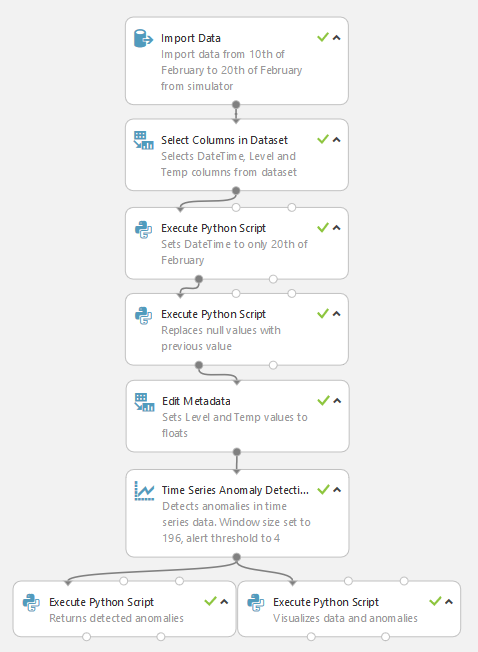
\includegraphics[width=0.5\textwidth]{timeSeriesAnomalyDetection}
                \caption{System setup using time series anomaly detection module}
                \label{fig:timeSeriesAnomalyDetection}
            \end{figure}
            
            We want to explore what kind of anomalies the Azure time series anomaly detection can detect by trying to find the anomalies marked in the dataset in section \ref{timeSeriesData}. 
            \par
            Next, we will explore if the twitter anomaly detection algorithm can detect the anomaly in the simulator dataset and in the on anomaly test dataset from section \ref{timeSeriesData}.
        }
            
        \subsection{Time Series Anomaly Detection with Twitter Algorithm} \label{timeSeriesADTwitter}
        {
            The twitter anomaly detection algorithms is a part of an open-source R package, which aims to detect anomalies in a wide variety of contexts. The package has two different types of anomaly detection functions, one for time series anomaly detection and one for vectors of numerical data. The vector anomaly detection function makes it possible to detect anomalies if timestamps are unavailable \cite{twitterGitHub}. 
            \par
            The time series anomaly detection function requires a dataframe with one timestamp column, and one with numerical data as input, while the vector anomaly detection algorithm only requires a column with numerical data \cite{twitterGitHub}. In addition to these inputs, the algorithm has some settings. Among them, these are the most important in our case:
            \begin{itemize}
                \item Maximum number of anomalies that will be detected (percentage of the data)
                \item Directionality of the anomalies to be detected
                \item Level of statistical significance to accept an anomaly
            \end{itemize}
            First the algorithm will be used to try to detect the anomaly in the simulator dataset. Next, the algorithm will be tested by exploring which of the anomalies in the data described in section \ref{timeSeriesData} it can detect.
        }
    }
    
    \section{Experiment B: Anomaly detection} \label{anomalyDetectionMethod}
    {
        When trying to detect anomalies in a system we can look at each feature individually, like in section \ref{prSignalAD}, or at complex, multi-feature anomalies. When doing so, we are no longer interested in detecting when a single signal is abnormal, but detecting anomalies in the combination of the features. In such a case, an anomaly can be an abnormal boolean state or numeric value at a given time or a combination of several features being abnormal. The approach of detecting anomalies on the combination of features is more complex due to the higher number of dimensions in the data, but can potentially give useful insights to anomalies which even a skilled operator might not be able to spot. 
        \par
        The first part of this section will consider anomaly detection on a simple and ideal two-dimensional dataset created for this specific experiment. 
        \par
        Second, we will look at data from Intelecy's simulator. The simulator data is more complex than the first experiment. It has higher dimensions and is not ideally distributed.
        \par
        At last, a real industrial dataset, known as \gls{secom}, will be tested. This is known to be a challenging dataset for supervised classification \cite{supervisedMLsecom}, which indicates that a unsupervised approach will be even more difficult.
        
        \subsection{Anomaly detection on ideal data} \label{fakeAD}
        {
            The created data will be introduced and described, and an explanation of the problem will be given. Further, the idea and the experiment will be illustrated.
            
            \subsubsection{Data}
            {
                To get an understanding of how the \gls{ocsvm} mentioned in section \ref{svmTheory}, performs on various types of data, we will start with a two-dimensional dataset. The dataset will consist of two types of points. Normal state or inlier data will be normally distributed around two points, diagonally placed to each other, on the two-dimensional plane. The anomalies or outliers will be uniformly spread along the perpendicular diagonal. A set of 200 inlier points is generated for training, further, a set of 40 inliers and a set of 20 outliers are generated to validate the model. This is shown in \figref{fakeDataAD}.
                \par
                One of the advantages of this test, is that the problem is easier to visualise than typical real problems, due to its low-dimensional nature. Being able to visually inspect each result will enable easier optimisation and tuning of the parameters, thus adjust the decision curve. 
                
                \begin{figure}[H]
                    \centering \includegraphics[width=0.75\textwidth]{anom-fake-data}
                    \caption{Ideal data}
                    \label{fig:fakeDataAD}
                \end{figure}
            }
            
            \subsubsection{Experiment with one-class SVM}
            {
                As a part of understanding the advantages and drawbacks of a unsupervised approach, and the \gls{ocsvm}, the number of incorrectly classified points for each dataset is calculated after each train and validation. These numbers will help us understand the strengths and weaknesses of each parameter setting and manually improve the model by re-training with new parameters.
                \par
                From \figref{fakeDataAD}, we can see that abnormal points and normal points can occur close to each other, which is believed to cause a fine line between too high and too low sensitivity.
                \par
                We will run the data through the algorithm and visualise the results for each test as shown in \figref{fakeOptiAD}. The first execution will be run with the default parameters for the \gls{ocsvm}. After this, we will try to optimise the result based on visual inspection. At last, we will do two extra tests to show the model when over-fitted and under-fitted to amplify the pitfalls that must be avoided with \gls{ocsvm}.
                
                \begin{figure}[H]
                    \centering 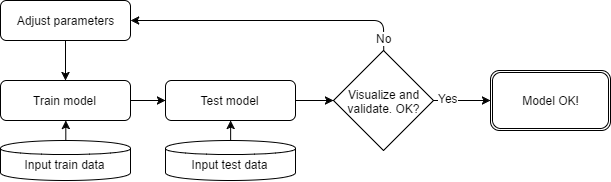
\includegraphics[width=0.75\textwidth]{anom-fake-opti}
                    \caption{Optimisation/ generalisation process on ideal data}
                    \label{fig:fakeOptiAD}
                \end{figure}
            }
        }
        
        \subsection{Simulator anomaly detection} \label{simuAD}
        {
            \subsubsection{Definition of anomalies} \label{defAnomalies}
            {
                As pointed out in section \ref{anomaliesTheory}, anomalies are defined as deviations from what is expected or irregularity from the norm. 
                To be able to detect anomalies in the simulator, we first need to define normal behaviour in this specific problem. To simplify this process, we defined that all data produced by the simulator in automatic mode are normal. With this baseline defined, we can assume that all values deviating from the typical cycles in automatic mode, are anomalies. Now we are able to label the data with its class, normal or abnormal. 
                \par 
                Setting the simulator to manual mode, enables us to provoke anomalies by manually tweaking operational settings.
                The training data that we ultimately want to retrieve from the simulator should contain only normal state, automatic mode operation. In contrast, the test data will contain a mix of normal state data and various types of tweaked anomalies. The anomalies will help us understand what the algorithm is able to detect, and what it fails to detect. \Figref{baselineSimAnomalies} abstractly shows a set of signals from the simulator where the red areas are anomaly labels.
                
                \begin{figure}[H]
                    \centering 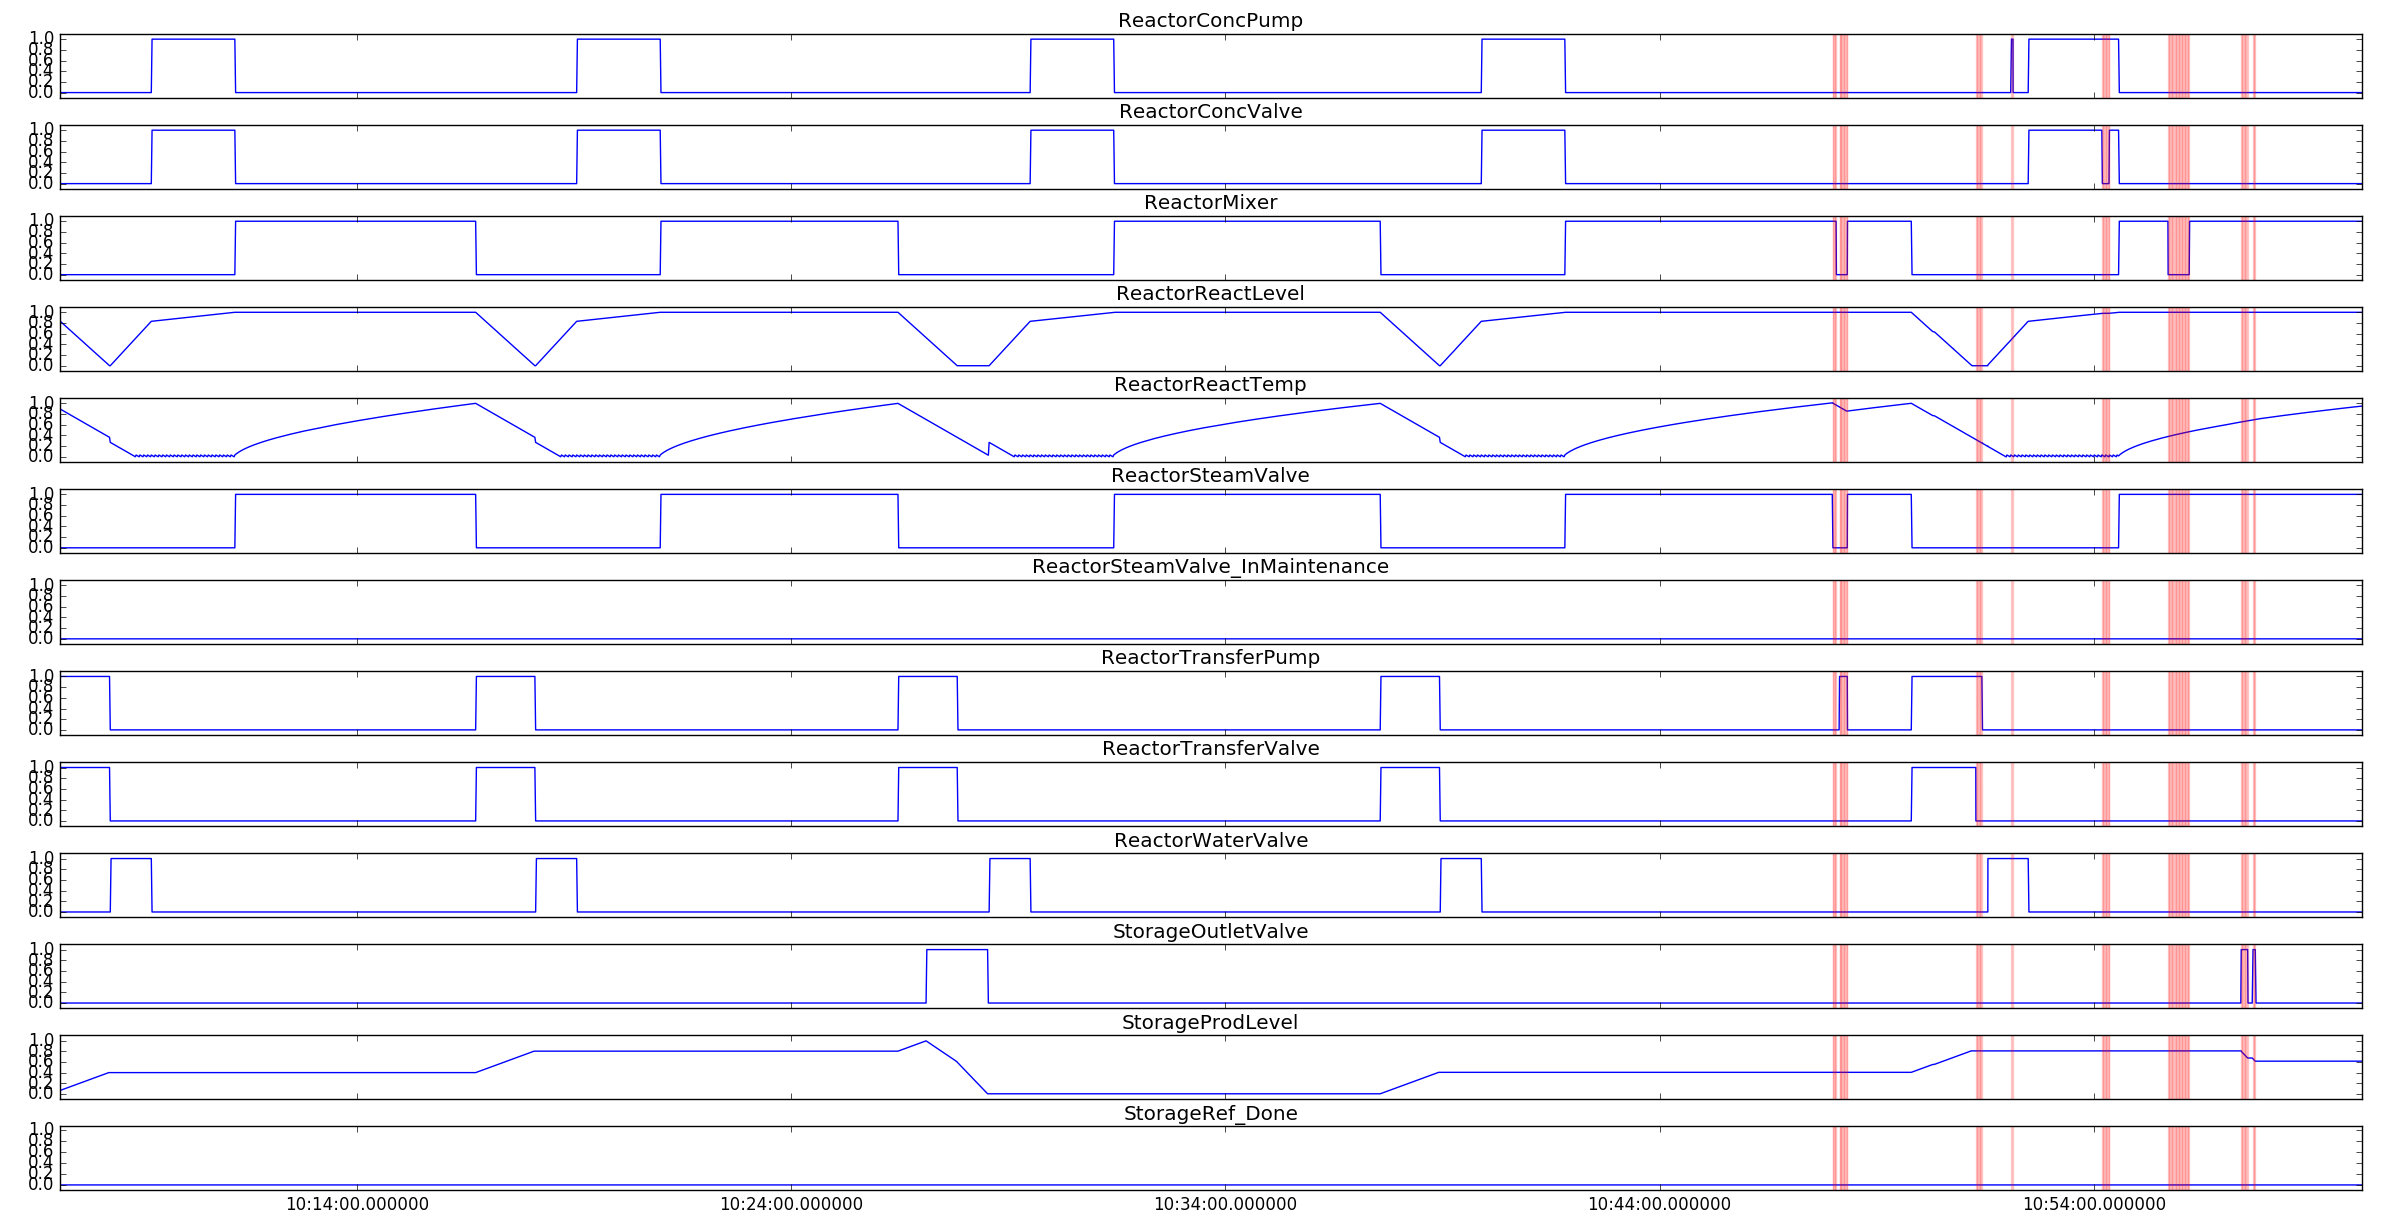
\includegraphics[width=\textwidth]{BaselineSimulatorData}
                    \caption{Simulator data and baseline for anomaly detection on the data} \label{fig:baselineSimAnomalies}
                \end{figure}
            }
            
            \subsubsection{Data and pre-processing} \label{simuAnomDPP}
            {                
                For anomaly detection on the simulator, 18 fields of normal state values are collected. These are data from one reactor logged for three days. The fields consist of a timestamp, numeric sensor values, numeric settings values, binary equipment states, binary input states, i.e. buttons, and binary production states. Some of the fields are highly relevant to detect anomalies according to our specified definition in section \ref{defAnomalies}, some fields are less useful, and some are completely non-descriptive. For instance, the state of the "automatic - manual" mode switch will add no value to an anomaly detection, since we want the algorithm to detect anomalies regardless of which operational mode the system is in, and also with the same basis. Another example of non-descriptive fields are the level alarm settings, these fields can be directly used in a logical “IF”-statement to check if the current value is above or below the limit, which requires no machine learning techniques.
                \par
                It is essential to remove the low-significance fields mentioned above, as training with these is likely to confuse the machine learning algorithm and reduce the precision, rather than improving it \cite{appliedPredictiveModeling}.
                \par
                To continue preparing the data for learning, several more steps are required. Some of which can be executed even before any further knowledge extraction. As stated in section \ref{simulator}, the fields are logged in delta. Since we know that the last seen value has not changed, we can keep this value in the dataset until the next time it changes, as described in section \ref{missingData}. After removing the unnecessary fields and forward filling values with respect to delta logging, the remaining data can be further analysed. 
                \par
                Since the data are temporal, i.e. time-series data, features in time domain are used. Higher order features introduces a new element of description of the data. Visual inspection of the data lead to the theory that rolling difference with fixed sized windows could better describe the behaviour of the system with respect to anomalies. Rapid response to sudden changes in amplitude is interpreted by the rolling difference.
            }
            
            \subsubsection{Experiment with one-class SVM}
            {   
                As mentioned in section \hyperref[oneclassSVM]{\ref*{oneclassSVM}}, the \gls{ocsvm} needs a training dataset consisting of only one class, which typically is the normal state of a system. Therefore, we need to be sure that the training data are within the corresponding definition. Our definition is, as previously suggested, normal state is when running in automatic mode – anomalies occur when operation deviates from the automatic sequences and values. To simulate anomalies, a labelled dataset has been created. These labels imply anomalies of different nature and occur both in binary and numeric features. 
                \par
                To verify the results, we test the model on the previously unseen, labelled dataset that was created in advance. A problem with verifying the results with a dataset that contains various types of anomalies is that these anomalies can have different importance, and the problem thereby have multiple objectives, in means of scoring. A model could have a good score, even though it only detects numerical anomalies and never detects binary anomalies, i.e. imbalance between anomaly types.
                \par
                \Gls{ocsvm} is one of few one-class \glsdesc{ml} algorithms that comes in the \gls{skl} package for Python. The parameters mentioned in section \ref{svmTheory}, need to be optimised for each problem, but if unspecified, some common values are set as default. Our approach to optimising the pre-processing settings and the algorithm parameters is based on the trial and error method. At first the dataset is used as is, directly from the initial pre-processing, with no added features or further feature selection techniques. This is run with \gls{skl}'s default parameters, to use as a reference for further optimisation. This gives useful insights of whether one-class classification is a feasible approach to this specific problem. Further, we need to tune the hyperparameters to yield a good solution on unseen data. 
                \par
                \Gls{skl} comes with several hyperparameter optimisation algorithms. Both grid search and randomised search are available in the package and are ready to use, but they search for the optimal solution based on a pre-defined scoring metric. The problem with this, in our case, is that the scoring metrics do not consider the types of the anomalies that are detected, which is essential in the multi-objective optimisation problem. 
                For this, a hyperparameter optimisation loop is written. The optimisation loop iterates through a range of parameters, and trains with all combinations of these parameters, and validate the result with the manually labelled test set. This will let us visualise the predictions for each iteration, and compare them by manually inspecting the results, and therefrom decide which results to keep and which to reject based on its performance on each type of anomaly. To reduce the amount of saved results that need to be manually inspected, a precision criteria has been set to greater than 0.5. All predictions with a lower precision will be rejected automatically. The principle of the loop is shown in \figref{optLoop}.
                                
                \begin{figure}[H]
                    \centering \RecustomVerbatimEnvironment{Verbatim}{BVerbatim}{} \inputminted{python}{thesis/Code/for_code.py}
                    \caption{Hyperparameter optimisation loop}
                    \label{fig:optLoop}
                \end{figure}
                
                \par
                Running the different combinations of original and new features through the hyperparameter optimisation loop will result in a list of stored settings that are comparable with respect to both setup and settings. Results from one combination of features can be compared to another combination. This will enable us to understand each feature's impact on the parameter settings and further do a feasibility study of algorithm adaptability to different features and problems.
               \par
               Combinations of features that were tested:
               
               \begin{itemize}
                   \item Normalised original features, numeric and binary.
                   \item Normalised original features, numeric.
                   \item Normalised original features, numeric and binary. Rolling difference with window = 1, numeric.
                   \item Normalised original features, binary. Rolling difference with window = 1, numeric.
                   \item Rolling difference with window = 1, numeric and binary
                   \item 5 component \gls{pca} of original features, numeric and binary.
               \end{itemize}
            }
        }
        
        \subsection{Anomaly detection on SECOM dataset} \label{secomAD}
        {
            The last anomaly detection experiment is executed on a real industrial dataset from a semiconductor manufacturing plant. Here, we will explain the pre-processing and the \gls{ocsvm} experiments on the dataset.
            \par
            It has to be noted that the \gls{secom} dataset represents a very challenging problem. As argued in Thorsten Wuest's Ph.D. Research; the fact that the \gls{secom} dataset was published as part of the “causality challenge” suggests that classification will not be an easy task \cite{supervisedMLsecom}. The baseline results of classification performance published in accordance with the \gls{secom} dataset by McCann \cite{pmlr-v6-mccann10a} corresponds with the findings of Kerdprasop \cite{kerdprasop2011data} investigating classification performance of the same dataset. These findings indicate that one-class classification will be even more challenging.  
            
            \subsubsection{Data and pre-processing} \label{secomADdpp}
            {
                In section \ref{secomData}, the dataset is described according to the available information, and it is mentioned that it has labels for classes. Since this experiment is supposed to consider unsupervised, one-class classification, we first need to split into a train set and a test set. Further, the train set should consist of only inlier data. To achieve this, we first remove all vectors or lines labelled anomalous. After the outliers are removed from the train set, we need to remove the label, since the \gls{ocsvm} only takes features as input, as shown in section \ref{mlImpl}. 
                \par
                The next step is to start pre-processing. This process is only based on the train set, since any information from the test set should be unseen until we do the predictions. The initial dataset contained 591 features, 1567 samples and a considerable amount of null values. Since the data are not in time series, we can remove vectors or samples missing more than a certain percentage of its values. In this case we used 6\% as the missing ratio limit. All rows missing more than 6\% of its observations will be rejected. When the rows are removed, we will check each features variance. Features with variance equal to zero are rejected and removed, due to their lack of descriptive power. Further, we will handle columns with a high missing values ratio as explained in section \ref{pre-processing-theory}. As a rule of thumb, features missing values for more than 60\% of its samples are considered unusable. This is just a rule of thumb, and might be a weak assumption, but for this feasibility study experiment we can assume that it is correct. Last, since \gls{ml} algorithms depend on numerical inputs for its calculations, we need to do something about the remaining empty cells. There are several approaches to handling these missing values. One of them is, as described in section \ref{knowledge-discovery-methods}, replacing them with zero. This is what we will do for this experiment.
                \par
                When the pre-processing routine is defined, we can apply the same operations to the test set. An illustration of the pre-processing routine is shown in \figref{secomPreProcessing}
                
                \begin{figure}[H]
                    \centering 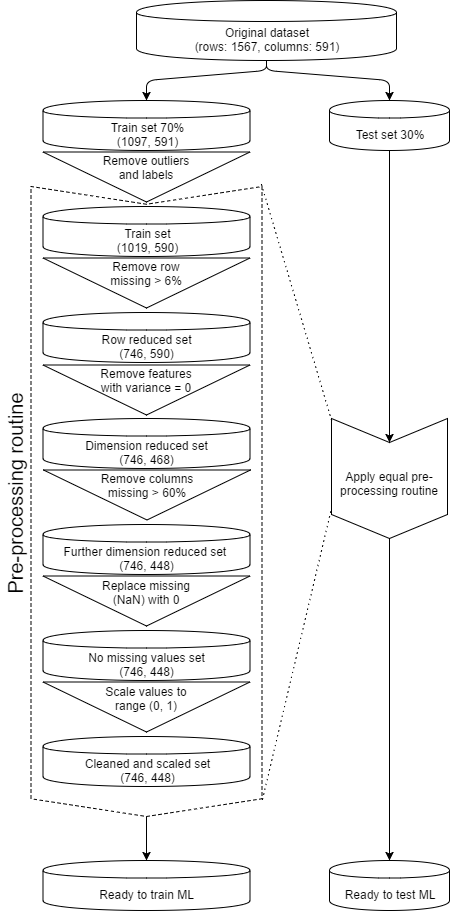
\includegraphics[width=.45\textwidth]{anom-secom-pre-process}
                    \caption{\gls{secom}: Pre-processing process}
                    \label{fig:secomPreProcessing}
                \end{figure}
                
                Since optimisation must be based on new data, other than the training set, we will split the test set in to two parts of 50\% each, one optimisation set, and one validation set. This will help in avoiding the use of validation data for optimisation, thus avoid over-fitting. 
                \par
                To get a more in-depth understanding of the data, we can look at their distributions. In \figref{secomRandDists} we randomly selected nine signals and plotted their histograms. These histograms show us the distributions of the features' values and can tell us whether values are uniformly spread or have some sort of shape, i.e. Gaussian, that the algorithm might be able to learn. 
                        
                \begin{figure}[H]
                    \centering 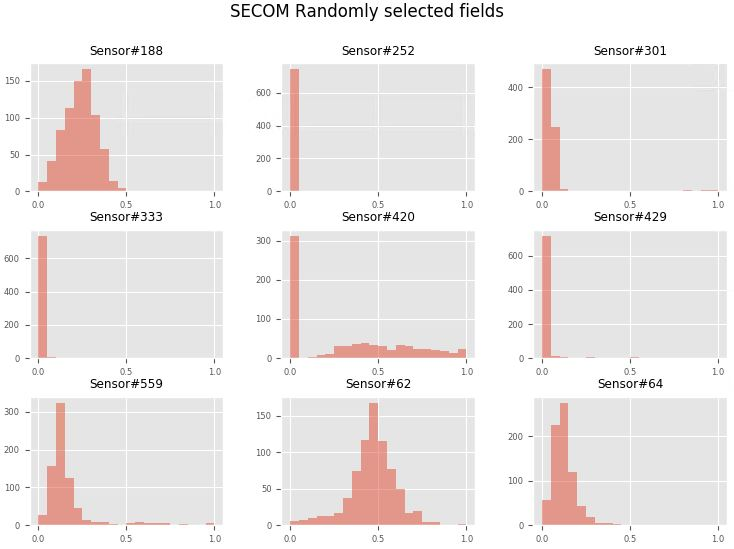
\includegraphics[width=\textwidth]{anom-SECOM-rand-fields}
                    \caption{\gls{secom}: Randomly selected sensor distributions}
                    \label{fig:secomRandDists}
                \end{figure}
                
                %Anyway, here are a few (22 / 448 normally distributed with p-val $>$= 0.05) normal dist figs:
                Since patterns are essential to \gls{ml}, we want to understand whether any of our features are normally distributed with p-value\footnote{value of statistical significance.} greater than 0.05. If any features are normally distributed, we would also like to know how often they occur in the dataset. By performing the test on each single signal, we can create a new dataset only containing the normally distributed signals.
            }
            
            \subsubsection{Experiment with one-class SVM}
            {
                After the dataset is cleaned and prepared, we are able to start testing the detection algorithm. To do initial tests, we proceed with the same approach as with the previous datasets; starting with the default parameter settings of the \gls{ocsvm}. This will again indicate whether the approach is feasible, and act as a reference for further improvement. 
                \par
                When the initial results are analysed, the hyperparameters for the algorithm likely need to be optimised. For this, we do a grid search based for-loop, as shown in \figref{optLoop}. This loop will be run with a precision criteria based on the optimisation set. The iterations with the highest precision will be verified with the validation set. The top precision scores and the corresponding hyperparameters will be saved and shown. In addition, we will create a confusion matrix, mentioned in section \ref{scoringMethods}.
            }
        }
    }
    
    \section{Experiment C: Classification} \label{experimentClassification}
    {
        As described in section \ref{classificationTheory} classification models attempts to find the correct category for new data. In these experiments we want to distinguish between normal and abnormal instances. We will test and compare three different classification algorithms for both of the datasets.\par
        In the first part we will look at classification on the data from the simulator, described in section \ref{simulator}. 
        \par
        In the second part we will look at classification on the \gls{secom} dataset, described in section \ref{secomData}.
        
        \subsection{Simulator classification experiment} \label{simulator-classification-experiment}
        {
            The simulator dataset is collected from a virtual process running on a server, and the data generated from this process are logged to a database (section \ref{simulator}). The dataset does not contain any labels for different classes or anomalies so we had to define it.
            
            \subsubsection{Definition of abnormal}
            {
                To be able to distinguish the normal from the abnormal we need to define what is normal, and here we will use the same definition as in section \ref{defAnomalies}, which is when the simulator operates in auto mode. 
                \par
                The data are collected from the simulator over three days. There are 18 fields and a total of 332 567 rows, where 84 rows are defined as abnormal. A 19th field is introduced and is the label for the two classes. 1 represents anomalies and 0 represents normal.
            }
            
            \subsubsection{Pre-processing} \label{pre-process-simulator}
            {
                As mentioned in section \ref{simulator}, the data are logged in delta, and we will use forward fill to replace the missing values with the last known value (section \ref{knowledge-discovery-methods}). Further there are some of the fields that does not add any value to the dataset, and these are removed. The removed fields are fields with only one value (0 variance) and the field representing the operational mode (auto/manual). When the fields with missing values are filled and the useless fields are removed we normalise the dataset between -1 and 1 by using equation \ref{normalisation-eq} and \ref{scaling-eq}.
                \par
                Further we take the pre-processed dataset and split it into training and test set. We use 2/3 of the dataset to train and 1/3 for testing. To keep the class ratio, we use a stratified split, as mentioned in section \ref{training}.
            }
            
            \subsubsection{Verification}
            {
                $F_1$ measure, precision and accuracy (section \ref{methods-for-scoring}) is used to evaluate the prediction performance. From these scores we can tell how well the different algorithms perform on the dataset.
            }
            
            \subsubsection{Algorithm experiments}
            {  
                In this experiment we will test three different algorithms for classification, and the goal is to compare the results from these algorithms.
                \par
                In section \ref{nearest-neighbour} we can see that the \gls{nn} algorithms can be used to classify a new data point based on the class of the nearest neighbour in the training set. In this experiment the \gls{knn} algorithm (section \ref{knnTheory}) will be used to classify because of its ability to include more than one neighbour in the decision making. The number of neighbours used in this experiment is: 1, 2, 10 and 15.
                \par
                A consideration when using \gls{knn} is how to calculate the distance to the nearest neighbours. In section \ref{knnTheory} three approaches for computing the distance are described. In this experiment K-D tree and Ball tree will be used. The Brute force approach on such a large dataset consumes a lot of memory.
                \par
                The Gradient Boosting algorithm is in this experiment used as a classifier (section \ref{GradientBoostingTheory}). The algorithm can be tuned with many different parameters, but in this approach only the 'max\_depth' (section \ref{GradientBoostingTheory}) parameter will be tuned. This parameter decides the maximum depth of the individual regression estimators \cite{gradientBoostingClassifier}. A grid search will be performed to find the best value for the 'max\_depth' parameter. 
                \par
                The \gls{mlpc} algorithm is an \gls{ann} for classification. The output of the algorithm is the predicted class. In this case the algorithm will only output labels found in the training set. 
                \par
                In this experiment the algorithm will be tested with different number of hidden layers, and a grid search (section \ref{HyperparameterOptimisation}) will be used to find the optimal set of perceptrons. The grid search will be performed with these sets of hidden layers: (100, 50), (80, 40), (60, 30), (50, 25), (40, 20), (25, 10).
            }
        }
        
        \subsection{SECOM classification} \label{secom-classification-experiment}
        {
            The \gls{secom} dataset contains 589 fields with sensor measurements, one field with a timestamp and one field with the label. The number of rows in the dataset is 1567 (section \ref{secomData}). The big difference between the simulator and \gls{secom} dataset is the number of fields. The \gls{secom} dataset contains over 32 times the number of fields, which makes it a more complex problem.
            
            \subsubsection{Pre-processing}
            {
                The initial dataset contains 931 416 datapoints, and of these there are 47267 missing values (section \ref{pre-processing-theory}). The missing values needs to be handled, and the same approach as described by Wuest \cite{supervisedMLsecom} is used. This approach consist of 4 steps, as shown in \figref{secomPreProcess}.
                
                \begin{figure}[H]
                    \centering 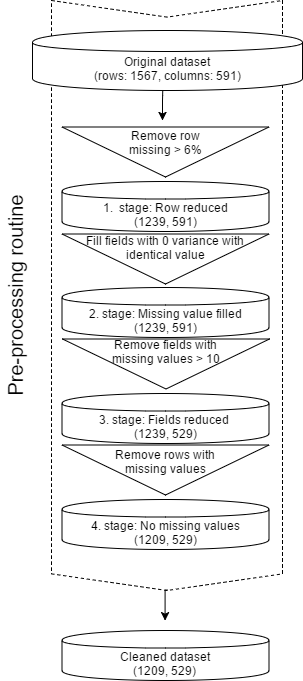
\includegraphics[width=0.4\textwidth]{SECOM-Pre-Process-Steps}
                    \caption{Pre-Processing steps for SECOM dataset}
                    \label{fig:secomPreProcess}
                \end{figure}
                
                \begin{enumerate}
                    \item Remove all the rows with more than 6\% missing values.
                    \item Replace missing values with otherwise identical values.
                    \item Remove all fields with more than 10 missing values.
                    \item Remove remaining rows with missing values.
                \end{enumerate}
                
                After these steps are performed the dataset is cleaned for missing values and have 529 fields and 1209 rows. In the remaining dataset we are left with 1125 passes and 84 fails. \par
                Further, to reduce the number of fields in the dataset all fields with 0 variance are removed, as they might reduce the performance of the algorithms \cite{appliedPredictiveModeling}. The cleaned dataset is then normalised between -1 and 1 by using equation \ref{normalisation-eq} and \ref{scaling-eq}. \par
                \gls{pca} is introduced to further reduce the number of fields, and the experiment will test the use of 10, 20, 40, 80 and 160 \gls{pca} components. \par
                The last ting to do is to split the dataset into training and test set, and the same approach as in section \ref{pre-process-simulator} is used.
            }
            
            \subsubsection{Validation}
            {
                As in section \ref{simulator-classification-experiment}, to verify the results from the tests the $F_1$ measure, precision and accuracy (section \ref{methods-for-scoring}) is calculated from a confusion matrix. From these scores we can tell how well the different algorithms perform on the dataset.
            }
            
            \subsubsection{Algorithm experiments}
            {
                As for the simulator dataset algorithm experiments (section \ref{simulator-classification-experiment}) this experiment will also test three different algorithms for classification. The goal is also the same.
                \par
                We will use the \gls{knn} algorithm the same way as in the simulator experiments. The best result regarding number of neighbours, will be tested using \gls{pca}.
                \par
                The \gls{gbc} will also be used the same way as in the simulator algorithm experiments, and when the best performing max\_depth parameter is found, this will be used when testing with the use of \gls{pca}.
                \par
                The \gls{mlpc} algorithm approach will, as in the simulator algorithm experiments, be tested with different number of hidden layers. A grid search (section \ref{HyperparameterOptimisation}) will find the best performing set of perceptrons out of these: (1000, 500), (500, 250), (250, 100), (150, 50), (100, 50), (100, 20). When the best performing hidden layer set is found, it will be used when testing with the use of \gls{pca}. 
            }
        }
    }
    
    \section{Experiment D: Event Prediction}\label{EventPredictionChap3}
    {
        Section \ref{concept} explained that the goal of event prediction is to predict when a breakdown or fault will occur, or when maintenance is needed. We will explore methods for predicting such events through this experiment. 
        \par 
        First, the turbofan engine degradation dataset (section \ref{nasaData}) is used to explore different approaches, pre-processing techniques, machine learning models and filtering techniques. Secondly, the experience from the first experiment will be used on the battery dataset (section \ref{batteryDataset}). We will take some of the \gls{ml} models that performed the best on the engine degradation dataset, and test them on the battery dataset to see if they adapt to other problems.
        
        \subsection{Prediction of RUL - Turbofan engine degradation dataset}\label{EngineRULProcedure}
        {
            The case with NASA turbofan engine degradation simulation dataset has the objective to predict the \gls{rul} for several engines, as explained in section \ref{nasaData}. Finding a solution that predicts the \gls{rul} in the best way, will depend on comprehensive testing with different features and pre-processing techniques as well as different regression models and the settings for them. 
            \par
            Section \ref{crisp-dm} explained that the \gls{crisp-dm} process is our preferred approach to use for our experiments in the project. Since no specifications are given on the engines and no information is given on what the operational settings and sensors are, this case needs a data driven approach. We need to start with the data understanding phase. 
            \par
            Given the operational settings, we will explore if the engines run in different operational modes, by using scattering and clustering. Scattering the operational settings will hopefully give an indication of possible operational modes. The clustering model, K-means (section \ref{K-MeansClusteringTheory}) will be used to extract these modes.
            \par
            Next, we will learn about the sensor data by looking at data quality reports (section \ref{dataQualityReport}). Before extracting features and making predictions, we need to setup testing routines for the experiments. 
            
            \subsubsection{Setup}
            {
                Setting up firm and good testing routines is important. The NASA dataset consists of 3 datasets, but only the training set has the actual \acrfull{rul} in it. The \gls{rul} is given by inverting the cycle count for each engine, since it is known that the engine breaks down at the last cycle. In this project, we use the training set provided and split it into a training set and a test set, as proposed in section \ref{training}.  The set consists of 218 units, we randomly choose 145 units for training, and the remaining 73 units for testing, resulting in a training set of 67\% and a test set of 33\%. To be able to reproduce the result, and be sure that the \gls{mse} is improved during testing we use a fixed random seed to be sure that the same units are used in each experiment. \Gls{mse} (equation \ref{mse-eq}) will be used to evaluate performance and improvement of the predictions between the tests. Since \gls{mse} is not very easy to interpret, \gls{mae} (equation \ref{mae-eq}) will be used to set prediction performance in perspective.  
            }
            
            \subsubsection{Feature experiments}
            {
                The feature experiments will be tested with an \gls{ann} of the type \gls{mlp} (section \ref{annTheroy}) for regression. A grid search (section \ref{HyperparameterOptimisation}) was executed, and the settings we got from this was used.
                \par 
                Initially, the original features will be tested, which is a good starting point to evaluate the importance of pre-processing. Next, operational mode acquired from clustering will replace the operational settings. The amount of cycles spent in each operational mode, for each run, will also be tested as a feature. These features are evaluated before exploring if we can reduce the number of sensors to improve the predictions. We will analyse which sensors show sign of degradation and use them as inputs. In addition, we will add features with the moving window functions, mentioned in section \ref{movingWindow}. Our theory is that including these features, can improve predictions, since they give an indication of the previous values in a time series dataset. \par 
                Feature combinations will be normalised using equation \ref{normalisation-eq} or normalisation by operational mode. Normalisation by mode means extracting all values in each operational mode, for every column, and normalising with equation \ref{normalisation-eq}, based on those. \Figref{NormaliseByMode} shows the function used for normalising by mode.
                
                \begin{figure}[H]
                    \centering \RecustomVerbatimEnvironment{Verbatim}{BVerbatim}{} \inputminted{python}{thesis/Code/NormaliseByMode.py}
                    \caption{Function for normalising based on operational mode}
                    \label{fig:NormaliseByMode}
                \end{figure}
                
                The best set of features will be used for testing several \gls{ml} models.
            }
            
            \subsubsection{Machine learning experiments}\label{NASAmlExperiment}
            {
                After exploring potential features and pre-processing techniques, we will explore if the \gls{mlp}, can be outperformed by other regression algorithms, or by a \gls{mlp} with other settings. We have chosen different types of algorithms to see if any types outperforms the other. Regression algorithms that will be tested:
                
                \begin{itemize}
                    \item Linear models (section \ref{LinearModelsTheory})
                    \item \gls{mlp} (section \ref{annTheroy})
                    \item Random Forest Regressor (section \ref{RandomForestTheory})
                    \item \gls{gbr} (section \ref{GradientBoostingTheory})
                    \item Ada boost Regressor (section \ref{AdaBoostTheory})
                    \item K-neighbour Regression (section \ref{knnTheory})
                    \item Support Vector Regression (section \ref{svmTheory}) 
                \end{itemize}
                
                Most machine learning algorithms have a lot of settings that greatly impact the prediction result. Optimising these settings can be complex, so for this we will use grid search (section \ref{HyperparameterOptimisation}) to optimise the algorithms.
            }
            
            \subsubsection{Filtering experiments}
            {
                The predictions from the machine learning algorithms will probably be rather noisy. Therefore, we will try to use a moving average filter (section \ref{fir}) to see if this can improve the \gls{mse}. The moving average will be implemented by using the moving window function described in section \ref{fir}.
            }
        }
        
        \subsection{Classification - Turbofan engine degradation dataset} \label{classificationTurbofan}
        {
            After we have predicted the \acrfull{rul} on the turbofan engine degradation dataset, we want to do a classification on it instead, to see if this will give us a better result. To do this we will follow the same procedure as in section \ref{EngineRULProcedure}, when it comes to testing different features and pre-processing techniques. This means that the setup will be the same as in the previous section, but the algorithms will be different. Algorithms that will be tested is: 
            
            \begin{itemize}
                \item \gls{svc} (section \ref{svmTheory})
                \item \gls{lsvc} (section \ref{svmTheory})
                \item \acrfull{knc} (section \ref{nearest-neighbour})
                \item \gls{nb} (section \ref{naiveBayesTheory})
                \item \gls{sgd} (section \ref{LinearModelsTheory})
                \item \acrfull{mlp} (section \ref{annTheroy})
                \item \acrfull{gbc} (section \ref{GradientBoostingTheory})
            \end{itemize}
            
            The main difference besides the algorithms, is when we train the models. When we predict the \gls{rul} in section \ref{EngineRULProcedure} we train with the actual \gls{rul}, but we cannot do this when using classifiers. Instead we will train with data that are 0 when the actual \gls{rul} is above a fixed threshold, and 1 when it is below. This means that we will detect when there are less than a given amount of cycles left of the life. To test our result we will use the accuracy score (see equation \ref{accuracy}). In addition to this we will set a second threshold to see if the models can detect the first threshold before it reaches the second, for example we detect that it is less than 100 cycles left before it is less than 50 cycles left. This is to be able to make sure that a company have enough time to order new parts before the system fails, as it often is unwanted to have too many spare parts in stock, and even less wanted to have an unplanned stand-still.
        }
        
        \subsection{Prediction of RUL - Battery dataset}
        {
            The battery dataset described in section \ref{batteryDataset} has the same objective as the turbofan engine degradation simulation dataset, which is to predict the RUL. Introducing a second dataset will indicate if the methods for predicting \gls{rul} are adaptable to other problems and to see what can be adapted from one experiment to another.
            \par
            Experiments on the battery dataset will follow the same procedure as for the first dataset from section \ref{EngineRULProcedure}. The aim is to use a data-driven approach for achieving good predictions instead of physics-based modelling. Eker compares prognostics datasets in his benchmarking paper, where the battery dataset is considered hard to perform data-driven approach on \cite{PrognosticsDatasetBenchmark}. We hope to achieve promising results, that indicate that it can be reasonable to reuse models and knowledge from the previous experiment. Since we wish to use a data-driven approach we will not study the batteries themselves in detail.
            \par
            To validate and measure performance on the predictions we will use \gls{mse} (equation \ref{mse-eq}) and visual inspection, which is a reasonable approach since the dataset is so small. \Gls{mae} (section \ref{mae-eq}) is used to give a perspective of the prediction performance. Since only 4 batteries are available, we will see if good predictions can be made by training on two of them, and predicting on the two remaining ones. We assume that it can be difficult to make accurate predictions with so few examples. Two and two of the batteries are quite similar, therefore training with 3 batteries can make the model over-fit to that type. 
            
            \subsubsection{Feature experiments}
            {
                The dataset has a more complex structure than the engine degradation set, and will require some work before simple predictions can be made. To predict the \gls{rul} we will combine charge and discharge cycle to predict remaining discharge cycles until the capacity is below 1.4 Ahr. Simple features to extract will be ambient temperature, capacity, estimated electrolyte resistance and estimated charge transfer resistance, since these are single values in their cycle type. The remaining values in each cycle are time series data through the entire cycle, such as measured voltage through a charge cycle. Possible features to extract from these variables will be considered by visually analysing them throughout the battery life. 
            }
            
            \subsubsection{Machine learning experiments}\label{BatteryMLChap3}
            {
                The features extracted in the previous section will be tested in different combinations, using two of the best performing machine learning models from the engine degradation experiment (\gls{mlp} and \gls{gbr}). The models setting will be optimised using grid search (section \ref{HyperparameterOptimisation}). 
            }
            
            \subsubsection{Filtering experiments}
            {
                To further improve the predictions, similar filtering methods as the ones tested in the engine degradation experiment, in section \ref{EngineRULProcedure}, will be used.
            }
        }
    }
    
    \section{Benchmarking Python versus Microsoft Azure ML Studio} \label{benchmarking}
    {
        In the experiments we have mentioned above we will use both Python and Microsoft Azure ML Studio. Therefore we want to measure the time used to run a model in both environments, so that we can compare them with each other. This will be done by recreating one of the experiments that we have done in Python, in Azure. Then we will measure the time used for each step in the experiment as well as the total time used. In this case we will use linear regression on the NASA turbofan engine degradation dataset. Linear regression is chosen because we found similar functions in both Python and Azure. Naming the columns and saving the dataset as a .csv file will be done in Python before it is uploaded to Azure. 
        \par
        We will recreate as much as possible with existing modules in \gls{ml} Studio. If there are no existing modules for some of the steps, we will use the Python script module. When using existing modules, there is not always the option to adjust as many settings as what is available in Python, so these will be set as equal as possible. The setup is shown below:
        
        \begin{figure}[H]
            \centering
            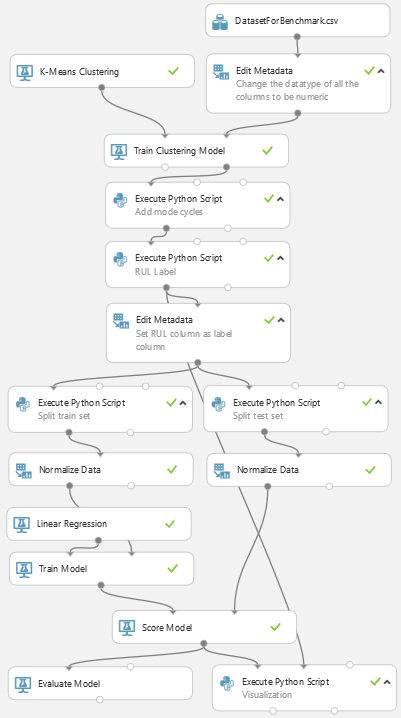
\includegraphics[width=0.5\textwidth]{LinearRegression}
            \caption{Linear regression setup in Azure}
            \label{fig:azureLinReg}
        \end{figure}
        
        As seen in \figref{azureLinReg} there are some steps that we had to use Python scripts to be able to recreate. The duration of each operational mode is a feature we have added, that cannot be created with standard modules in Azure. The same goes with adding the \gls{rul} as an own column in the dataset, and there is not an existing module for visualising the result. We have also used Python scripts to split the dataset into training and test datasets although there is a module for splitting data. This is because we want to recreate the experiment in Python as much as possible, therefore it is important that we have exactly the same split in Azure as we do in Python so that we can compare the performance. We will also measure the time consumption of the split module. We have used two scripts to split the data, and this is because the Python script module in Azure do not have the opportunity to return a dataframe on each of its outputs as the second output is reserved for visualising. 
        \par 
        The times we will measure is; clustering, adding mode cycles, \gls{rul} labelling, splitting, normalising, training, prediction, evaluation, visualisation and the total time. We will also compare the \gls{mse} and \gls{mae}, as well as the visualisations, to check that the performance is similar. The split module in Azure has a variety of settings for how to split the dataset. In this particular problem it is important to split the dataset based on engine number, which is not possible using this module. If the built-in split module is used, we cannot visualise the predictions.
    }
}

\newpage
\chapter{Results}
{
    \section{Experiment A: Per signal anomaly detection}\label{PerSignalAnomRes}
    {
        In this section we will look into the results we got from the different methods we have tested for per signal anomaly detection. It will describe how and why we have tested out different settings for parameters, and show the results from different settings. 
        
        \subsection{Time Series Anomaly Detection with Azure}\label{AnomAzure}
        {
            Since the data we are working with are time series we decided that a good place to start would be to test the time series anomaly detection module already made in Azure. As mentioned in section \ref{timeSeriesAD} we started out with a window size of 196. We also started out with a threshold of 0.9, which seemed to be way to low based on the anomaly scores we got. Therefore we set it to 4 instead. The result is shown below:
            
            \begin{figure}[H]
                \centering
                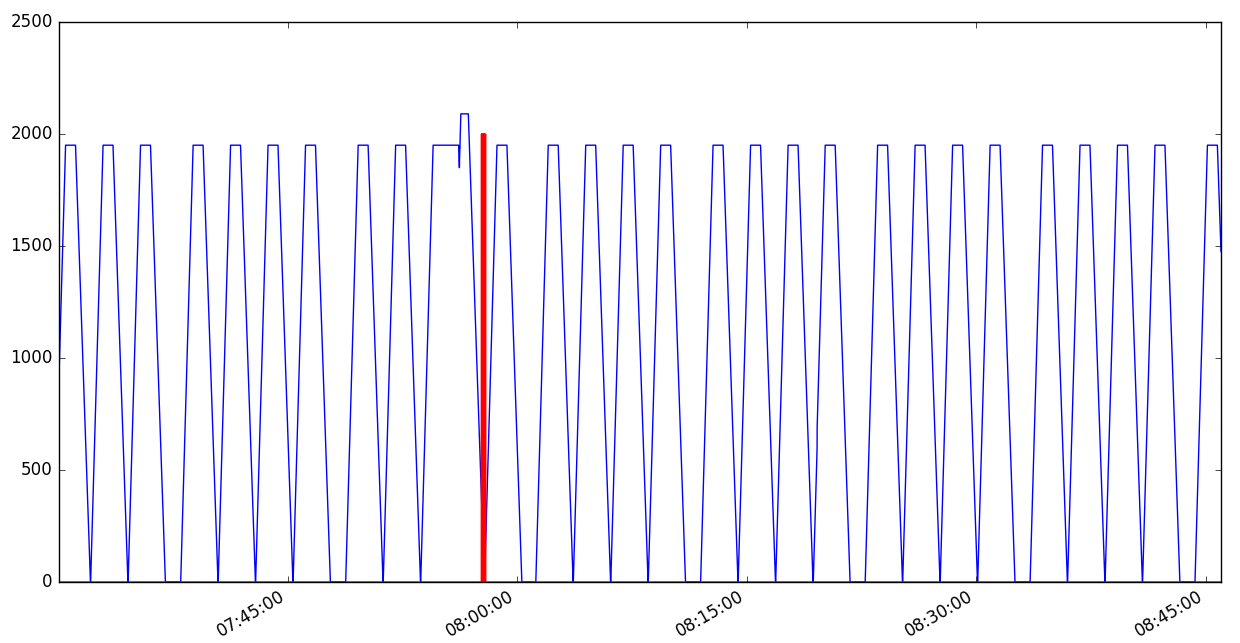
\includegraphics[width=\textwidth]{Window-196}
                \caption{Time series anomaly detection with window size 196}
                \label{fig:timeSeriesADWindow196}
            \end{figure}
            
            We also tested the setup shown in \figref{timeSeriesAnomalyDetection} with window sizes equal to a half period and two periods:
            
            \begin{figure}[H]
                \centering
                \includegraphics[width=\textwidth]{Window-98}
                \caption{Time series anomaly detection with window size 98}
                \label{fig:timeSeriesADWindow98}
            \end{figure}
            
            \begin{figure}[H]
                \centering
                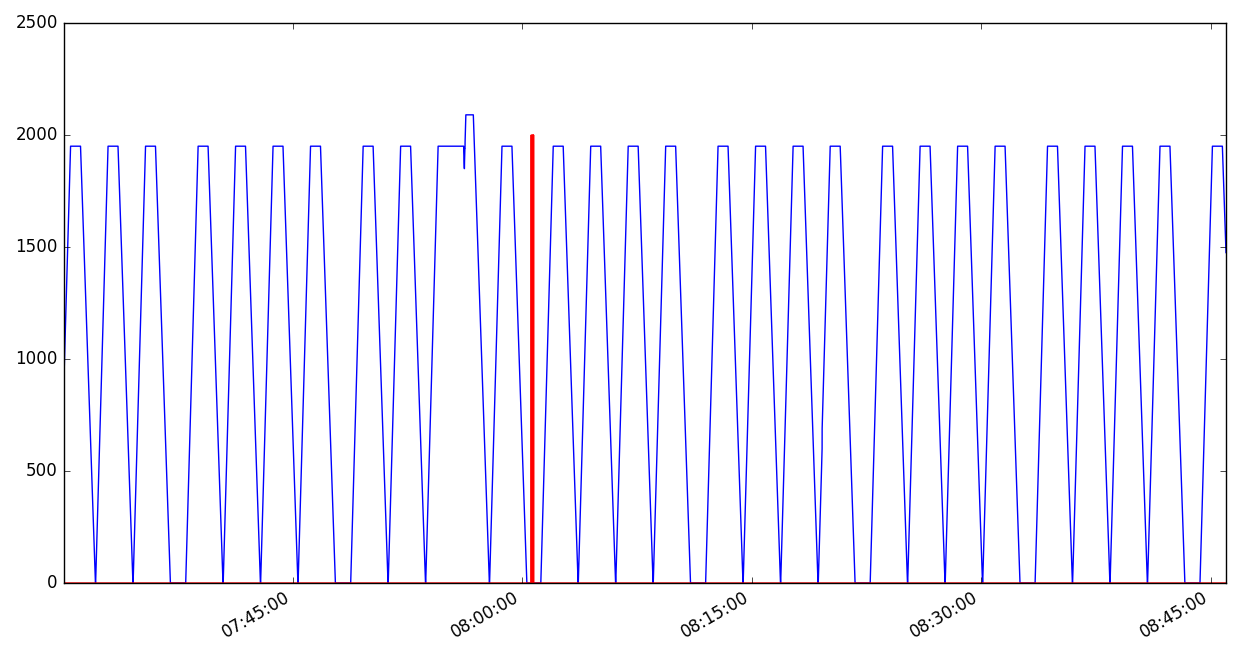
\includegraphics[width=\textwidth]{Window-392}
                \caption{Time series anomaly detection with window size 392}
                \label{fig:timeSeriesADWindow392}
            \end{figure}
            
            Since the figures shown above only visualises a small area of our dataset we do not see all alerts. For example when the window size was set to 196 we had a total of 12 alerts, where 8 of these were within the red area in \figref{timeSeriesADWindow196}. With a window size of 98 we had a total of 18 alerts, while when the window size was 392 we had a total of 8 alerts. The more alerts we got, the more sensitive the system was. We do not want the system to be too sensitive as that would generate a lot of alerts that are not really anomalies, but the system would have to be sensitive enough to be able to detect the anomalies.
            
            As mentioned in section \ref{timeSeriesAD} we made an anomaly in a dataset that consists mostly of normal data. This anomaly is the peak shown in the figures above that is a bit wider than the rest, and this is the anomaly that we wanted to detect. When looking at the figures with different window sizes we see that all of them detect an anomaly at a time near the actual anomaly. A problem with all of these results is that it seems as though it detects the anomaly a little late, actually after it occurred. Detecting an anomaly after it happened is not very useful for live monitoring, but it could be useful for a root cause analysis. To make it more suitable for live monitoring we decided to try to use the same module in combination with rolling kurtosis (section \ref{movingWindow}) instead of directly on the tank level. This gave us the following result with a window size of 196: 
            
            \begin{figure}[H]
                \centering
                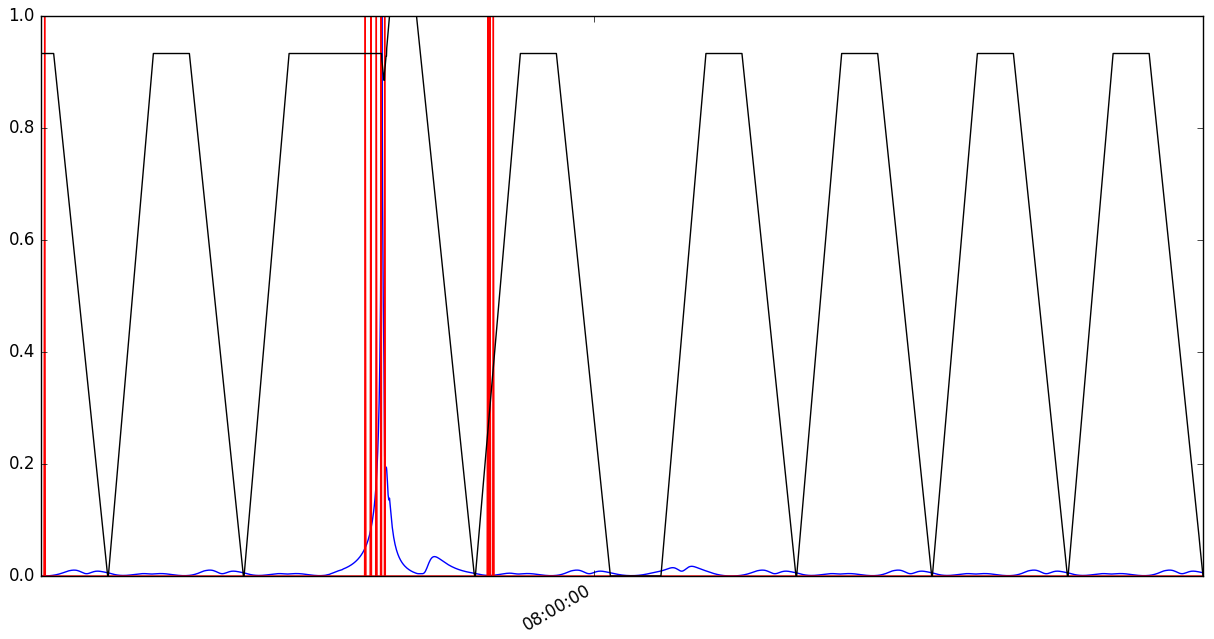
\includegraphics[width=\textwidth]{Kurtosis-Window-196}
                \caption{Time series anomaly detection with kurtosis, window size 196}
                \label{fig:timeSeriesADKurtosisWindow196}
            \end{figure}
            
            Now we can see that we get a lot of alerts in the middle of the anomaly, but we also get some alerts at other places. We actually got as much as 70 alerts in total, which is a lot more than previously. In other words we can see that the sensitivity of the system increased. Therefore we increased the window size to maximum (1000) to try to decrease the sensitivity, and got the following result:
            
            \begin{figure}[H]
                \centering
                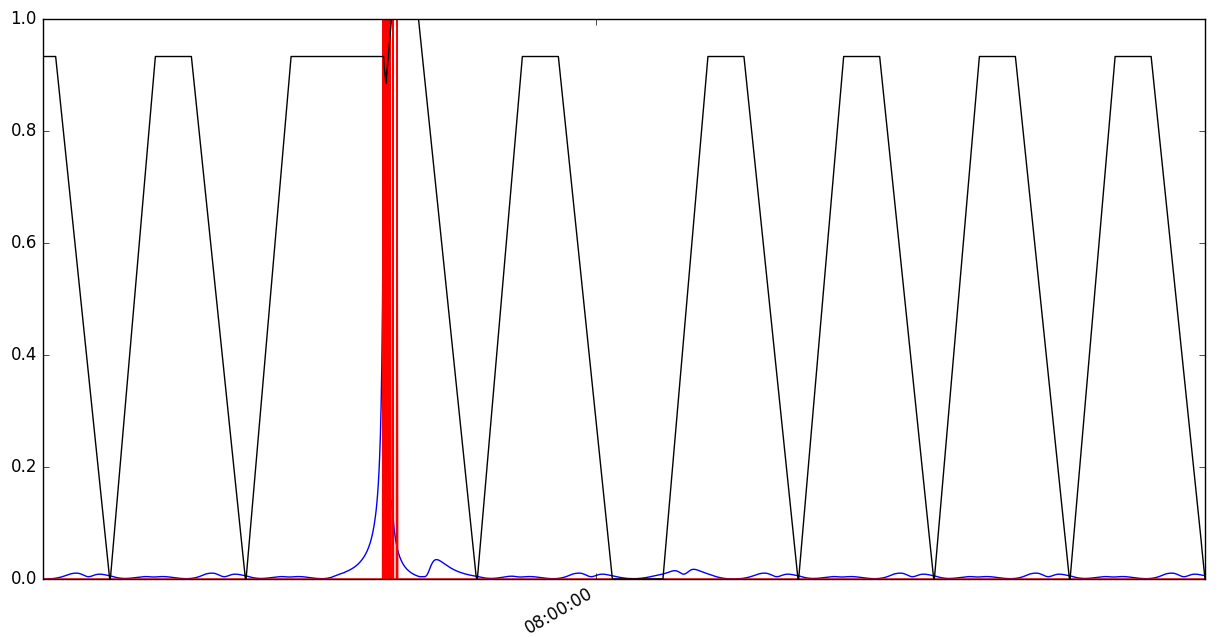
\includegraphics[width=\textwidth]{Kurtosis-Window-1000}
                \caption{Time series anomaly detection with kurtosis, window size 1000}
                \label{fig:timeSeriesADKurtosisWindow1000}
            \end{figure}
            
            This decreased the number of alerts to 14, and we can see that we still detect the anomaly very well (although a bit later than with window size 196).
            \par 
            After adjusting the settings for detecting the anomaly on the reactor level signal and achieving good results, we want to explore what more we can expect from the time series anomaly detection model by testing the algorithm towards the dataset in section \ref{timeSeriesData}.
            \par
            None of the anomalies were detected on the signals even though 100 different settings where tested. We need to test an alternative algorithm for time series anomaly detection on individual signals. 
        }
        
        \subsection{Time Series Anomaly Detection with Twitter algorithm}\label{AnomTwitter}
        {
            As mentioned in section \ref{timeSeriesADTwitter} time series anomaly detection on individual signals will be performed in this experiment using the twitter anomaly detection algorithm. The first test is on the tank level signal from the simulator dataset. 
            \par 
            Section \ref{AnomAzure} showed that the Azure time series anomaly detection model was able to detect an anomaly in the tank level. The best results was given when anomalies was detected on the rolling kurtosis of the level parameter. By using the rolling kurtosis and a window size of 196 as in the Azure experiment, the twitter anomaly detection algorithm, detected anomalies in the correct area. Visualisation of the detected anomalies is shown in \figref{AnomSimuTwitt}.
            
            \begin{figure}[H]
                \centering
                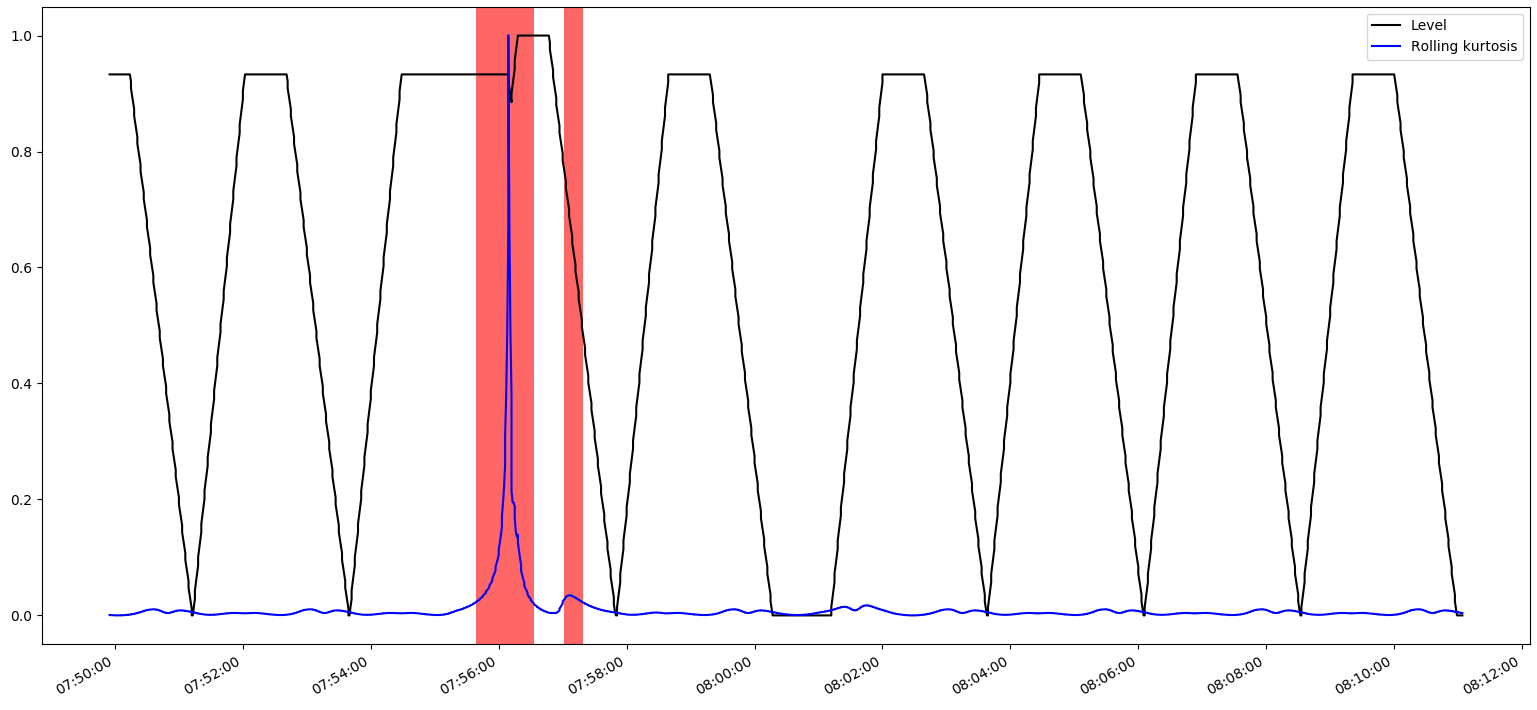
\includegraphics[width=\textwidth]{AnomSimuTwitt}
                \caption{Time series anomaly detection with kurtosis, window size 1000}
                \label{fig:AnomSimuTwitt}
            \end{figure}
            
            Next, we will explore the performance of the algorithm on the time series anomaly detection dataset introduced in section \ref{timeSeriesData}. The upcoming figures illustrates the created anomalies with navajo white and the detected anomalies with red.
            \par
            Anomaly detection performance on signal one from the dataset described in section \ref{timeSeriesData} is shown in \figref{AnomType1Res}.
            \begin{figure}[H]
                \centering
                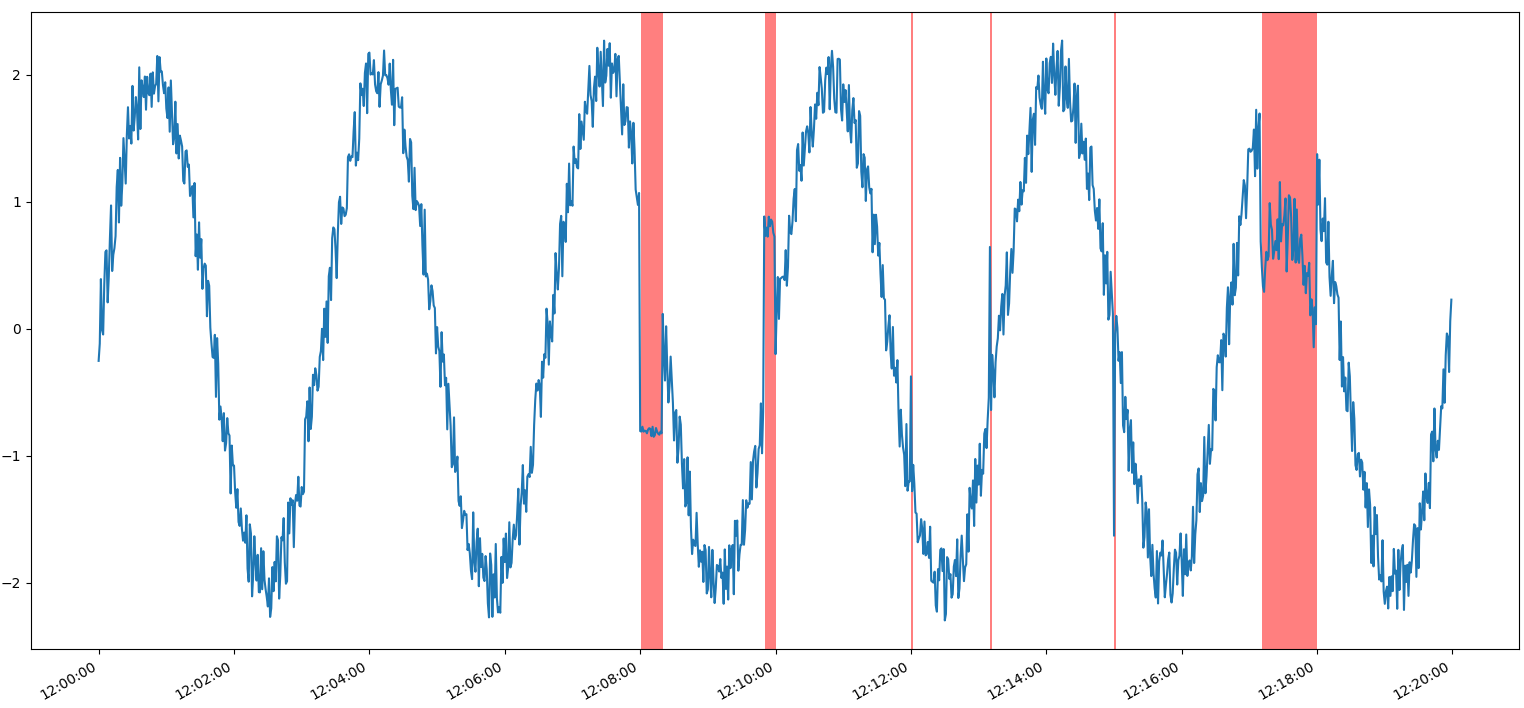
\includegraphics[width=\textwidth]{AnomType1Res}
                \caption{Detected anomalies on the first test signal}
                \label{fig:AnomType1Res}
            \end{figure}
            
            Detected anomalies on signal 2, 3 and 4 are indicated in \figref{AnomType2Res}, \figref{AnomType3Res} and \figref{AnomType4Res} respectively.
    
            \begin{figure}[H]
                \centering
                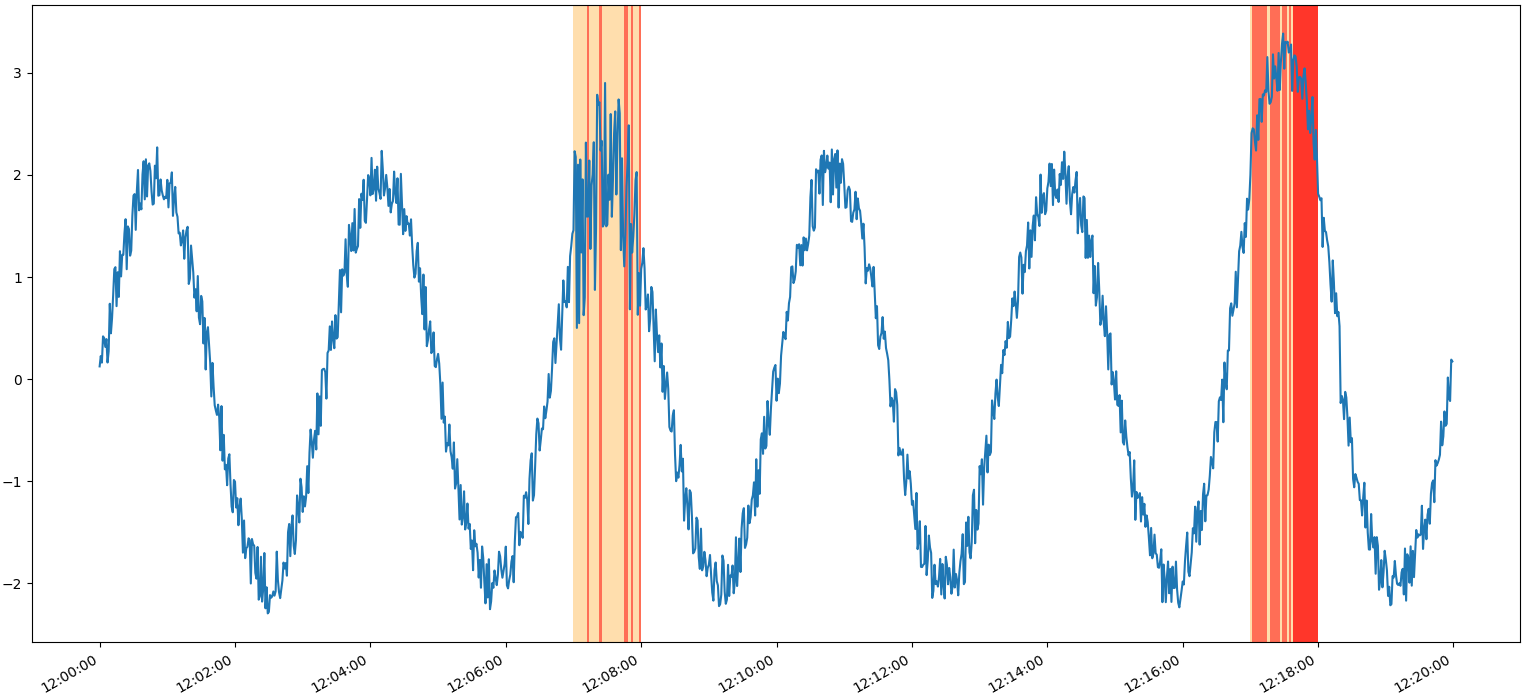
\includegraphics[width=\textwidth]{AnomType2Res}
                \caption{Detected anomalies on the second test signal}
                \label{fig:AnomType2Res}
            \end{figure}
            
            \begin{figure}[H]
                \centering
                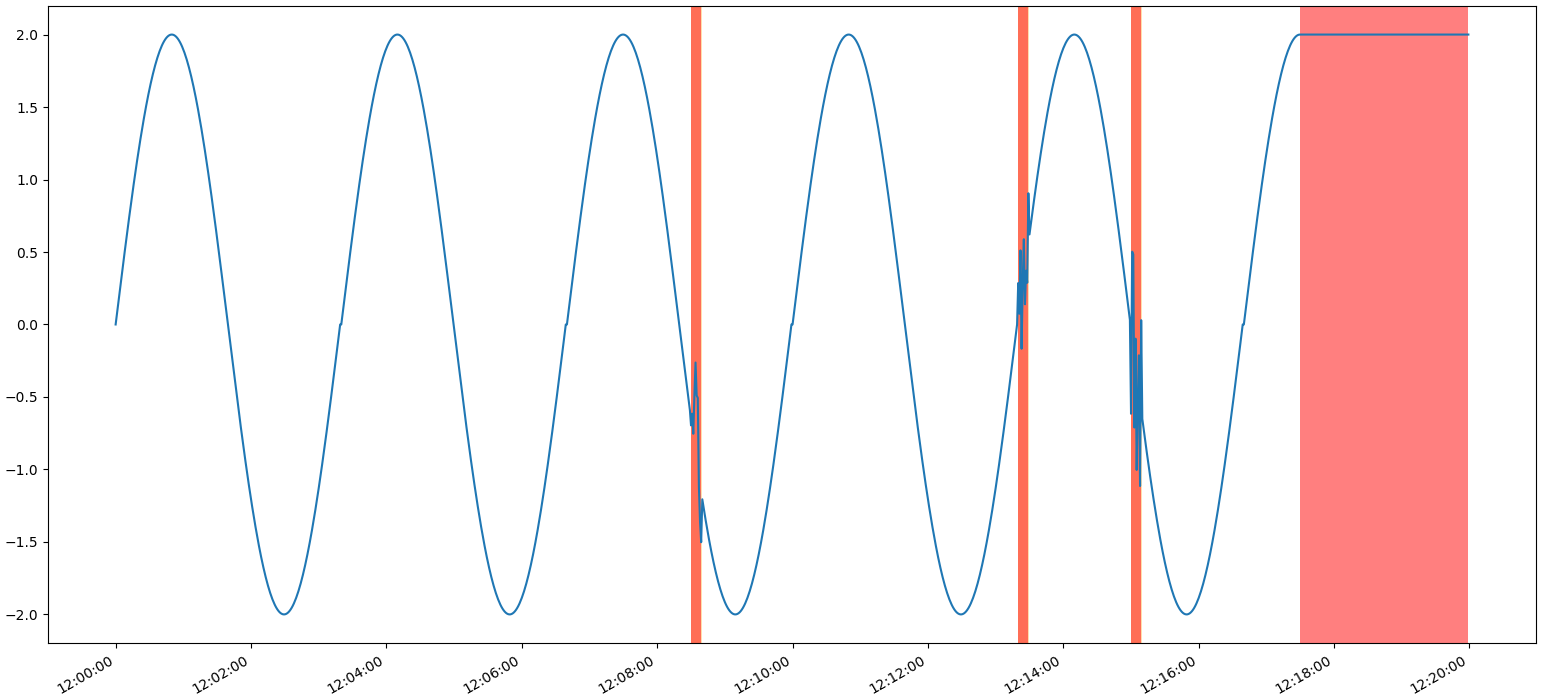
\includegraphics[width=\textwidth]{AnomType3Res}
                \caption{Detected anomalies on the thrid test signal}
                \label{fig:AnomType3Res}
            \end{figure}
            
            \begin{figure}[H]
                \centering
                \includegraphics[width=\textwidth]{AnomType4Res}
                \caption{No detected anomalies on the last test signal}
                \label{fig:AnomType4Res}
            \end{figure}
    
            \Figref{AnomType4Res} tell us that no anomalies are detected for signal number 4. A technique described in section \ref{detrend}, is to detrend the signal, by removing growth and then try to detect anomalies. The detrended signal is shown in \figref{AnomType5}.
            
            \begin{figure}[H]
                \centering
                \includegraphics[width=\textwidth]{AnomType5}
                \caption{The last test signal after detrending}
                \label{fig:AnomType5}
            \end{figure}
            
            Detected anomalies on the detrended signal are shown in \figref{AnomType5Res}.
            
            \begin{figure}[H]
                \centering
                \includegraphics[width=\textwidth]{AnomType5Res}
                \caption{Detected anomalies on the last test signal after detrending the signal}
                \label{fig:AnomType5Res}
            \end{figure}
            
            Having explored per signal anomaly detection, we want to see if anomaly detection on several signals or systems is possible. 
        }
    }
        
    \section{Experiment B: Anomaly detection}\label{AnomalyDetectionResult}
    {
        \subsection{Anomaly detection on ideal data}
        {
            The ideal data described in section \ref{fakeAD} consist of a dataset with two clusters of normal or inlier points for training, a set of normal points for validation, and a set of anomalies for validation. Predictions and  optimisation will proceed as illustrated in \figref{fakeOptiAD}. This optimisation process is used to let us visualise the decision line on top of the actual data and calculate the number of wrongly classified points for each set. 
            \par
            The first test is visualising the results from a prediction with default \gls{ocsvm} parameters. The results are visualised in \figref{defaultAD}. As can be seen in the figure, the prediction finds the centre of the clusters in the training data. It does also classify all outliers correctly. The problem is that the classifier suggests that 100 out of 200, or 50\% of the points in the training set are outliers. We can see that the decision line is well within the actual perimeter of the clusters and that many points from training data are outside the decision line. An interpretation of these results suggest that the model will be highly sensitive, and in practice give warnings at too many of the normal points, as mentioned as one of the anomaly detection challenges in section \ref{anomDetChallenges}. 
            
            \begin{figure}[H]
                \centering
                \includegraphics[width=0.75\textwidth]{anom-fake-default}
                \caption{Default One-class SVM on ideal data}
                \label{fig:defaultAD}
            \end{figure}
            
            After optimisation, we found that the parameters and results visualised in \figref{generalizedAD} are closer to what we want. Fewer of the training points are classified as outliers, and also fewer of the normal validation points are classified as anomalies. The model is still able to detect all outliers. This model can therefore be interpreted as a generalised model. Our suggested interpretation is also reinforced by the fact that all new points occurring within our new and wider decision line or area are classified as inliers, which implies a less sensitive model than with the default parameters.
            
            \begin{figure}[H]
                \centering
                \includegraphics[width=0.75\textwidth]{anom-fake-generalized}
                \caption{Generalised One-class SVM on ideal data}
                \label{fig:generalizedAD}
            \end{figure}
            
            After being able to produce a quite suiting, generalised model, we would like to have a look at the pitfalls that one might run into when using the \gls{ocsvm}. Since the results are also more difficult to visualise with increasing number of dimensions, we consider these pitfalls highly relevant.
            \par
            The first possible mistake we want to elaborate, which might occur when trying to create a "perfect" \gls{ml} model is over-fitting (section \ref{generalization}). This mistake happens when the decision line or field fits the training data to good. New, unseen points that deviate from the training data are then likely to be wrongly classified as outliers. An example of an over-fitted model is visualised in \figref{overfittedAD}. In this figure we can see that the purple points, unseen inlier data, are classified as outliers in 28 of the 40 examples. This model will be way too sensitive for any practical use, and can be interpreted as remembering the already seen data, instead of learning its pattern. 
                
            \begin{figure}[H]
                \centering
                \includegraphics[width=0.75\textwidth]{anom-fake-overfitted}
                \caption{Over-fitted One-class SVM on ideal data}
                \label{fig:overfittedAD}
            \end{figure}
            
            The other mistake which we would like to amplify the importance of avoiding, is under-fitting (section \ref{generalization}). This can be considered the opposite of the previously mentioned over-fitting problem. This happens when too few points are used for training, or when the \gls{ocsvm} is trained with wrong parameters. Technically speaking, low gamma leads to high variance models, and vice-versa. This is shown in \figref{underfittedAD}, and as the calculated errors in the figure shows, the figure is highly insensitive, and will fail to classify a considerable amount of the outliers correctly.
            
            \begin{figure}[H]
                \centering
                \includegraphics[width=0.75\textwidth]{anom-fake-underfitted}
                \caption{Under-fitted One-class SVM on ideal data}
                \label{fig:underfittedAD}
            \end{figure}
        
            Now that the principals and some strengths and weaknesses are explored, a more complex problem is needed. In the next section, we will test the \gls{ocsvm} on the simulator dataset, described in section \ref{simulator}.
        
        }
        
        \subsection{Simulator anomaly detection}
        {
            When it comes to anomaly detection on the simulator data, the combinations of features, and the hyperparameter optimisation loop described in section \ref{simuAD} were used. The combinations of features and parameters were optimised with a precision criteria. Parameters and results were kept for all tests with a precision greater than 20\%. The first test was executed with the default parameters of the \gls{ocsvm}, just like in the ideal data experiments. This time, unlike the ideal data experiment, the default parameters result was nowhere near a usable model. The model classified more than 50\% of the data points from the training set as outliers, even though only less than 1\% where actual outliers according to the definition, therefore, the model parameters were rejected. 
            \par
            After running the optimisation loop, the results improved. The results are visualised in \figref{simuADgood}, where the known anomalies are marked red. The width of the red areas is a measure of the anomaly's duration. The blue line shows the prediction. When the blue line is at "0", the model predicts that there are no anomalies in the data. "1" implies the detection of an anomaly. The red field at approximately 09:50 is an error where the reactor level remains at the same level instead of decreasing, when the outlet valve is open. The anomaly at approximately 10:40 indicates that the pump stopped during a process where it normally runs. Further, the anomalies between 10:50 and 11:10 are various types and combinations that were generated by tweaking the simulator in the graphical user interface and manual mode. Not all of these were detected. Precision, training time and the parameters used can be read from the figure.
            
            \begin{figure}[H]
                \centering
                \includegraphics[width=\textwidth, height=.42\textheight]{anom-simu-good}
                \caption{Simulator: Best results}
                \label{fig:simuADgood}
            \end{figure}
            
            One of our observations is that even after testing with all the combinations of features listed in \ref{simuAnomDPP}, the combination of rolling difference on numerical features and original binary features gave the only good results. The best precision achieved was 67\%, after running this particular combination through the hyperparameter optimisation loop.
            \par
            To check the robustness of this model, the \begin{math}\nu \end{math} (nu) parameter was slightly changed, and the test was executed again. This time, the precision was reduced from 67\% to 1\% and the training time increased from six seconds to 16 seconds. A graph of the predictions of the new, slightly modified model is shown in \figref{simuADnewNu}. Once again, some of the pitfalls when using the \gls{ocsvm} are disclosed.
            
            \begin{figure}[H]
                \centering
                \includegraphics[width=\textwidth, height=.42\textheight]{anom-simu-ok}
                \caption{Simulator: Minor change, unusable results}
                \label{fig:simuADnewNu}
            \end{figure}
            
            To further compare the results, we introduced the \gls{secom} dataset, which is a real dataset. Anomaly detection on this dataset will be tested in the next section.
        }
        
        \subsection{Anomaly detection on SECOM dataset}
        {
            In this section, a further study of the nature of the SECOM dataset is provided, before \gls{ml} models are tested. As described in \ref{secomADdpp}, a statistical hypothesis is formed and tested. The idea is to generate a dataset containing all features that are normally distributed, to look for patterns.
            \par
            The statistical test shows us that only 22 of the 448 features are within the definition of normal distribution. A sub set of the normal distribution features are shown in \figref{secomNormalDists}. This discovery leads to the theory that there are few concrete, recognisable patterns in the \gls{secom} dataset, which in turn might lead to low precision results, as described in the book "Identifying Product and Process State Drivers in Manufacturing Systems Using Supervised Machine Learning" \cite{supervisedMLsecom}.
            
            \begin{figure}[H]
                \centering
                \includegraphics[width=\textwidth]{anom-SECOM-norm-fields}
                \caption{\gls{secom}: Gaussian sensor distributions}
                \label{fig:secomNormalDists}
            \end{figure}
              
            The test was executed with the default parameters of  the \gls{ocsvm} at first, then with hyperparameter optimisation and a precision criteria, to save the results and the corresponding parameters. This test was done with the dataset, processed with the technique described in section \ref{secomADdpp}. This test resulted in no models good enough to pass the precision criteria.
            \par
            To find the results the algorithm was able to achieve, the precision criteria was changed. Instead of saving all results better than a defined limit, the loop was set to save the best result out of all the combinations. The best precision score was 5.6\%, which indicates that the model is not able to recognise any patterns in the data. The corresponding accuracy score was approximately 71\%, which sounds good. The problem with using the accuracy score in a class imbalanced dataset like the \gls{secom} is that always predicting the major class will yield a good accuracy, even though it is not useful for any practical implementation.
            \par
            Table \ref{simu-confusion} shows the confusion matrix of the best solution from this experiment. 
            \begin{table}[H]
                \centering
                \begin{tabular}{|c|c|c|}
                     \hline
                     \textbf{} & \textbf{Predicted true} & \textbf{Predicted false} \\ \hline
                     \textbf{Actual true} &  4 (TP) & 6 (FN)\\ \hline
                     \textbf{Actual false} & 68 (FP) & 181 (TN)\\ \hline
                \end{tabular}
                \caption{Confusion matrix with rolling difference on numeric features, window = 1, and binary features}
                \label{simu-confusion}
            \end{table}
                        
        }
        
        As we have explored the possibilities and difficulties in a scenario with unlabelled data and unsupervised \gls{ml}, we have found this to be a challenging topic. To exemplify the challenges, we want to re-do some of the experiments with supervised \gls{ml}, and compare the results. The next section, contains supervised classification experiments on both the simulator and the \gls{secom} dataset.
    }

    \section{Experiment C: Classification}\label{ClassificationResult}
    {
        This section addresses the results achieved from the classification experiment. It describes the different results we got from testing the three classification algorithms on the simulator and \gls{secom} dataset.
        \par 
        
        \subsection{Simulator dataset}
        {
            The data collected from the simulator does not contain any labels, so we applied labels to the data based on our definition of abnormal (section \ref{simulator-classification-experiment}). The dataset were split into a training set and a test set. Further the data was pre-processed according to section \ref{simulator-classification-experiment}. The missing data was handled and useless features was eliminated. The dataset achieved after pre-processing was tested with the three algorithms, and below is the results from the tests.
            
            \begin{table}[H]
                \centering
                \begin{tabular}{|c|c|c|c|}
                    \hline
                    \textbf{   Algorithm   } & \textbf{   Precision   } & \textbf{   Accuracy   } & \textbf{   $F_1$ measure   } \\ \hline
                     kNN (1) & 100\% & 100\% & 100\% \\ \hline
                     kNN (2) & 100\% & 100\% & 100\% \\ \hline
                     kNN (10) & 91,3\% & 99,9\% & 80,7\% \\ \hline
                     kNN (15) & 91,3\% & 99,9\% & 80,7\% \\ \hline
                     MLPC & 96,7\% & 99,9\% & 98,3\% \\ \hline
                     GBC & 100\% & 99,9\% & 94,5\% \\ \hline
                \end{tabular}
                \caption{The results from testing different classification algorithms on the simulator dataset}
                \label{tab:sim-results}
            \end{table}
        
            The \gls{knn} algorithm with one and two neighbours gave us a perfect classification of the dataset, where with ten and fifteen neighbours the precision went down. With ten and fifteen neighbours the algorithm predicted two normal instances as abnormal and 8 abnormal as normal. The same results was acheived with both the K-D three and Ball three (section \ref{knnTheory}) approach for calculating the nearest neighbours.
            \par
            Classification with the \gls{mlpc} algorithm gave a precision of 96,7\%, accuracy of 99,9\% and a $F_1$ measure of 98,3\%. When we look at the predictions the algorithm only mis-classified one instance. It predicted 1 normal instance as abnormal, and based on the number of predictions (113073) it must be considered to be good enough. The results was achieved when using 25 perceptrons in the first hidden layer and 10 in the second hidden layer. These settings were found using a grid search (section \ref{HyperparameterOptimisation}). 
            \par
            The last test was with the \gls{gbc} algorithm. The results shows that all of the instances it predicted to be abnormal was correct, but it missed 3 of the abnormal instances. The grid search gave a max\_depth of 12. The results is from using this parameter.
            \par
            As seen in the result, the algorithms is able to classify the dataset with acceptable results. According to the scoring a \gls{knn} algorithm with one or two neighbours will give 100\% reliable results if similar abnormal instances is presented to the algorithm. The \gls{mlpc} algorithm gave the second best results, only one fault classification, and is the algorithms which is most adaptable to retraining and corrections when new unseen abnormal instances is presented to the algorithm.
            \par 
            In the next section the results from classification on the \gls{secom} dataset are presented.
        }
        
        \subsection{SECOM dataset}
        {
            The \gls{secom} dataset already came with labels so we did not need to add these. We had to pre-process the dataset to handle missing values, and the method described in section \ref{secom-classification-experiment} was used. The \gls{secom} dataset is known to be a challenging dataset for supervised classification \cite{supervisedMLsecom}. This is visualised in \figref{secom-PCA-plot}.
            
            \begin{table}[H]
                \centering
                \begin{tabular}{|c|c|c|c|}
                    \hline
                    \textbf{   Algorithm   } & \textbf{   Precision   } & \textbf{   Accuracy   } & \textbf{   $F_1$ measure   } \\ \hline
                     kNN (1) & 20,8\% & 89,5\% & 18.8\% \\ \hline
                     kNN (2) & 100\% & 93,2\% & 6,7\% \\ \hline
                     kNN (10) & NaN & 93,2\% & Nan \\ \hline
                     kNN (15) & NaN & 92,6\% & NaN \\ \hline
                     MLPC & 20\% & 88,6\% & 20,3\% \\ \hline
                     GBC & 33,3\% & 92,7\% & 6,2\% \\ \hline
                \end{tabular}
                \caption{The results from testing different classification algorithms on the SECOM dataset}
                \label{tab:secom-results}
            \end{table}
            
            As we can see from table \ref{tab:secom-results} the \gls{knn} algorithm can at best, when using one neighbour, classify five of the fails correctly, which is only 17,2\% of the fails. The algorithm also predicts 19 of the passes to be fails. When using two neighbours we get a precision on 100\% but as this only is based on one true positive it is not a good result. The $F_1$ measure of 6,7\% prooves this. The use of ten and fifteen neighbours results in that all instances is classified as passes, and can not be used.
            \par
            The \gls{mlpc} algorithms performs a little better than the \gls{knn} algorithm in the case of classifying the fails correctly, but on the other hand it predicts more of the passes to be fails. It predicted six fails correctly and 24 passes as fails. The results were generated with the use of 100 perceptrons in the first hidden layer and 20 in the second hidden layer. These were found by using a grid search (section \ref{HyperparameterOptimisation})
            \par
            By using the \gls{gbc} algorithm we was able to get a precision of 33,3\%, but the $F_1$ measure of 6,2\% indicates that this is not a good result. When looking at the numbers this becomes much clearer. The \gls{gbc} algorithm classifies 3 instances to be fails, of these only one was a fail. The results of the grid search gave a max\_depth of 1.
            \par
            The results from the tests shows that none of the algorithms can classify the dataset with a high precision, accuracy and $F_1$ measure. The results from using PCA to reduce the number of fields is presented in the following section. 
            
            \subsubsection{PCA}
            {                
                As mentioned in section \ref{secom-classification-experiment} PCA was introduced to reduce the number of fields, and the results are presented in table \ref{tab:secom-pca-results}.
                \begin{table}[H]
                    \centering
                    \begin{tabular}{|c|c|c|c|c|}
                    \hline
                    \textbf{   Algorithm   } & \textbf{   PCA   } & \textbf{   Precision   } & \textbf{   Accuracy   } & \textbf{   $F_1$ measure   } \\ \hline
                    \multirow{5}{*}{kNN} & 10 & 16,7\% & 89,1\% & 15,1\% \\ \cline{2-5} 
                     & 20 & 23,1\% & 91,2\% & 14,2\% \\ \cline{2-5} 
                     & 40 & NaN & 93\% & NaN \\ \cline{2-5} 
                     & 80 & NaN & 93\% & NaN \\ \cline{2-5} 
                     & 160 & NaN & 93\% & NaA \\ \hline
                    \multirow{5}{*}{MLCP} & 10 & 16,7\% & 89,1\% & 15,1\% \\ \cline{2-5} 
                     & 20 & 16,7\% & 91,2\% & 12,7\% \\ \cline{2-5} 
                     & 40 & 5,2\% & 91,2\% & 5,2\% \\ \cline{2-5} 
                     & 80 & 6,2\% & 91\% & 4,4\% \\ \cline{2-5} 
                     & 160 & 25\% & 91\% & 17,8\% \\ \hline
                    \multirow{5}{*}{GBC} & 10 & 33,3\% & 92,7\% & 6,2\% \\ \cline{2-5} 
                     & 20 & 100\% & 92,2\% & 6,7\% \\ \cline{2-5} 
                     & 40 & NaN & 93\% & NaN \\ \cline{2-5} 
                     & 80 & 25\% & 92,4\% & 6\% \\ \cline{2-5} 
                     & 160 & NaN & 93\% & NaN \\ \hline
                    \end{tabular}
                    \caption{Results from testing the algorithm  with PCA}
                    \label{tab:secom-pca-results}
                \end{table}
                When comparing the results in table \ref{tab:secom-pca-results} with table \ref{tab:secom-results} we can see that there is not really any improvement, even though the \gls{gbc} algorithm managed to get 100\% precision when 20 PCA components was used. The reason for the 100\% precision was that one fault was predicted correctly and non of the passes to be fault. The $F_1$ measure proves the bad performance. 
            }
        }
    }    
    
    \section{Experiment D: Event Prediction}\label{EventPredictionResult}
    {
        \subsection{RUL with Regression: NASA - turbofan engine degradation} \label{NASATurbofanRegr}
        {
            The NASA turbofan engine degradation dataset has as mentioned in section \ref{nasaData}, 21 sensor measurements and 3 operational settings of 218 units from an initial wear until breakdown. The actual \acrfull{rul} therefore spans linearly from start to end, making the last cycle number for every engine, the initial actual \gls{rul}. Since no information about operational modes is given it was necessary to explore the data to learn about the engines. 
            
            \subsubsection{Knowledge discovery}
            {
                It is given that the operational settings have considerable effect on engine performance, and therefore we explore if the settings can split up into operational modes. The scatter plot of the three operational settings shown in \figref{OP_Settings_PCA3D}, gives a clear indication that there are 6 different modes. 
                
                \begin{figure}[H]
                    \centering \includegraphics[width=0.7\textwidth]{OP_Settings_PCA3D}
                    \caption{Scatter plot of the three operational settings}
                    \label{fig:OP_Settings_PCA3D}
                \end{figure}
                
                To verify that there are infact 6 different operational modes and that the sensor measurements are dependent on the mode, we used 3 component \gls{pca} (section \ref{PCA}) of both operational settings and sensors measurements. As shown in \figref{PCA3D} the PCA components forms into six water drop shaped clusters when they are scattered.
                
                \begin{figure}[H]
                    \centering \includegraphics[width=0.7\textwidth]{PCA3D}
                    \caption{Scatter plot of the three PCA components obtained from sensors and settings}
                    \label{fig:PCA3D}
                \end{figure}
                
                The water drop form of the clusters gave us the idea that the thin part of each cluster could illustrate the wear of the engine. 
                \par
                To easily detect which operational mode an engine operates in, the K-means clustering algorithm (section \ref{K-MeansClusteringTheory}) with 6 clusters was introduced. By training and fitting the data into these clusters with the operational settings as inputs we could determine every cluster. \Figref{K-Means} shows the cluster centres as white crosses in combination with the scatter plot of a two component \gls{pca} on the entire dataset.
                
                \begin{figure}[H]
                    \centering \includegraphics[width=0.7\textwidth]{K-Means}
                    \caption{Cluster centers (as white crosses) and 2 component PCA scatter plot combined}
                    \label{fig:K-Means}
                \end{figure}
                
                After exploring and extracting knowledge about the engines operational mode, we explored the sensor data by generating a data quality report (section \ref{dataQualityReport}). All the values are of datatype float and had the same amount of present values, more information can be extracted from table \ref{nasaDQR}, that shows an small extract of the quality report.
                
                \begin{table}[H]
                    \centering
                    \begin{tabular}{|l|l|l|l|l|l|l|}
                        \hline
                        \textbf{}         & \textbf{Missing Value Ratio} & \textbf{Unique Values} & \textbf{Min} & \textbf{Max} & \textbf{Mean} & \textbf{Std. dev.} \\ \hline
                        \textbf{Sensor 1} & 0.0                          & 6                      & 445.0        & 518.67       & 472.86        & 26.46              \\ \hline
                        \textbf{Sensor 2} & 0.0                          & 1571                   & 536.65       & 644.43       & 579.60        & 37.39              \\ \hline
                        \textbf{Sensor 3} & 0.0                          & 11839                  & 1245.43      & 1614.66      & 1419.95       & 106.28             \\ \hline
                        \textbf{Sensor 4} & 0.0                          & 14713                  & 1029.49      & 1442.36      & 1205.67       & 119.55             \\ \hline
                        \textbf{Sensor 5} & 0.0                          & 6                      & 3.91         & 14.62        & 8.03          & 3.62               \\ \hline
                        \textbf{Sensor 6} & 0.0                          & 14                     & 5.71         & 21.61        & 11.60         & 5.45               \\ \hline
                        \textbf{Sensor 7} & 0.0                          & 2004                   & 136.75       & 555.72       & 282.47        & 146.54             \\ \hline
                        \textbf{Sensor 8} & 0.0                          & 880                    & 1914.85      & 2388.36      & 2228.05       & 145.58             \\ \hline
                    \end{tabular}
                    \caption{Extract of quality data report on the NASA dataset}
                    \label{nasaDQR}
                \end{table}
                
                The clustering and quality report is a part of the knowledge engineering, and is further used for extracting and generating features that can improve the prediction of \gls{rul}. Before running any predictions, the potential features mentioned below were extracted.
                
                \begin{itemize}
                    \item Replace operational settings with operational mode collected from K-means 
                    \item Run length in each mode for all engines. Every time an engine is in an operational mode the specific mode count is increased.
                \end{itemize}
                
                After feature engineering, we have 31 features available, operational setting 1-3, sensor measurements 1-21, operational mode and run time in operational mode 1-6. 
                \par 
                In section \ref{EngineRULProcedure} we explained that choosing the best solution is a complex problem where it is necessary to experiment with different pre-processing methods, features, machine learning models and their settings. The available features will be tested with a \gls{mlp} model (section \ref{annTheroy}) with optimised settings, acquired from a grid search (section \ref{HyperparameterOptimisation}).
                \par 
                The dataset is split up into a training and testing set, as described in section \ref{EngineRULProcedure}.
                \par
                Initially, four feature combinations are tested. The combinations are tested both with and without normalisation, as well as with normalisation based on operational mode. 
                \begin{itemize}
                	\item Operational setting and sensors (original features)
                	\item Sensors and operational mode
                	\item Sensors, operational mode and mode duration
                	\item Only mode duration
                \end{itemize}
                
                The predictions made with the first combination of features give a \gls{mae} at 51 and \gls{mse} at 3526. In average, the prediction misses with a positive or negative error of 51 cycles, which is too much. We wish to improve these predictions, and reduce the \gls{mse}. Table \ref{NASAFeatureCombosMSE} show the \gls{mse} of the other feature combinations.
                
                \begin{table}[H]
                    \centering
                    \begin{tabular}{|l|l|l|l|}
                    \hline
                    \multicolumn{4}{|c|}{\textbf{MSE - Simple feature combinations}} \\ \hline
                     & \textbf{Original} & \textbf{Normalised} & \textbf{Normalised by mode} \\ \hline
                    \textbf{Op. setting and sensors} & 3526 & 3727 & 3388 \\ \hline
                    \textbf{Sensors and mode} & 3343 & 1745 & 1712 \\ \hline
                    \textbf{Sensors and mode duration} & 1567 & 1172 & 1182 \\ \hline
                    \textbf{Only mode duration} & 1499 & 1437 & 1441 \\ \hline
                    \end{tabular}
                    \caption{Comparing MSE for feature combinations and normalisation}
                    \label{NASAFeatureCombosMSE}
                \end{table}
                
                As table \ref{NASAFeatureCombosMSE} clearly indicates, introducing the mode duration reduces the \gls{mse}. Normalising the features also contribute to improved predictions. Using a combination of sensor measurements and mode duration has reduced the \gls{mae} to 25.7, which in practice means that the mean prediction error has been reduced with about 50\%. \Figref{BasicFeaturePrediction} show an extract of predictions made with the three first combinations, without normalisation. It supports our assumption that introducing the mode duration improves our predictions.
                
                \begin{figure}[H]
                    \centering \includegraphics[width=1\textwidth]{PredictionNASA1D}
                    \caption{Actual RUL vs. predicted RUL using different features}
                    \label{fig:BasicFeaturePrediction}
                \end{figure}
            
                \Figref{NASAPredWithNorm} show predictions on two engines using the sensor values and mode duration both with and without normalisation.
            
                \begin{figure}[H]
                    \centering \includegraphics[width=1\linewidth]{PredictionNASA3}
                    \caption{Prediction using sensor values and mode duration both with and without normalisation}
                    \label{fig:NASAPredWithNorm}
                \end{figure}
            
                As mentioned in section \ref{nasaData}, the engine life varies between 128 and 356 cycles. Adding the mode duration as a feature creates a stronger correlation between the predictions and the average engine life. Units that fail after about 150 cycles are over-estimated, while units with a longer life than 180 cycles are predicted quite well. \Figref{NASAPredLongandShort} illustrates this, engine 205 has an actual life of 137 cycles, while engine 179 has an actual life of 226 cycles.
            
                \begin{figure}[H]
                    \centering \includegraphics[width=1\linewidth]{PredictionNASA4}
                    \caption{Prediction on engine with short life and long life}
                    \label{fig:NASAPredLongandShort}
                \end{figure}
                
                To make sensor values more valuable in predictions, the number of sensors is reduced. By analysing number of unique values in correlation with operational mode, sensor 1, 5, 10, 16, 18 and 19 seemed superfluous. Visually analysing the remaining sensors showed that especially sensor 3, 4, 7, 9, 11, 12 seemed to have an equal effect on RUL on both short and long life engines, when normalised by mode. \Figref{FiltSens11} shows that the value increases before the end of life, when normalising by mode, while \figref{NormNormSens11} shows that for traditional normalisation it shows a more unclear pattern. 
                
                \begin{figure}[H]
                    \centering \includegraphics[width=0.6\linewidth]{FiltSens11}
                    \caption{Sensor 11 normalised by mode, for short and long life engines}
                    \label{fig:FiltSens11}
                \end{figure}
                
                \begin{figure}[H]
                    \centering \includegraphics[width=0.6\linewidth]{NormNormSens11}
                    \caption{Sensor 11 normalised, for short and long life engines}
                    \label{fig:NormNormSens11}
                \end{figure}
                
                Predicting the \gls{rul} with the promising sensors and mode duration, normalised by mode, gives a \gls{mse} of 1148. Traditional normalisation gives a \gls{mse} of 1467. An example prediction of a short and long life engine is shown in \figref{FewSensorPrediction}. 
                
                \begin{figure}[H]
                    \centering \includegraphics[width=1\linewidth]{FewSensorPrediction}
                    \caption{Prediction for short and long life engines using sensor 3, 4, 7, 9, 11, 12 and mode duration}
                    \label{fig:FewSensorPrediction}
                \end{figure}
                
                Having found a set of features that perform well, it is necessary to explore the possibility to extract even more features from the existing ones. Experimenting with different combinations of features acquired from moving window functions (section \ref{movingWindow}), showed that calculating the rolling mean and difference for sensor 3 and 11 with a window at 4, improved the predictions. \Gls{mse} got reduced to 1120. \Figref{FewSensorPredictionWithFeatures} shows that predictions on short life engines are further improved.
                
                \begin{figure}[H]
                    \centering \includegraphics[width=1\linewidth]{FewSensorsWithFeaturesMeanDiffSens3and11}
                    \caption{Prediction for short and long life engines using few sensors, mode duration and rolling aggregations} \label{fig:FewSensorPredictionWithFeatures}
                \end{figure}
                
                Having explored a variety of pre-processing techniques and features combinations it is time to explore more machine learning models for regression, and try to optimise their settings.
            }
            
            \subsubsection{Machine learning models}
            {
                The previous section showed the result of knowledge discovery and feature experimentation using \gls{mlp}. So far, the best predictions are achieved when using mode duration and a reduced set of sensor measurements normalised by mode, as features. It resulted in a \gls{mse} at 1120 and \gls{mae} at 25.5. Further prediction improvements will be done by using the hyperparameter optimisation method, grid search (section \ref{HyperparameterOptimisation}), on the models in the selection from section \ref{NASAmlExperiment}. Section \ref{considerationChoosingAlgo} explained the importance of accuracy, training time and prediction time when choosing a \gls{ml} model. The upcoming tables evaluate these measures, \gls{mse} for accuracy, training time and time used to predict the 15252 samples in the test set, as prediction time.  
                \par
                Initially, linear models (section \ref{LinearModelsTheory}) in the \gls{skl} package where optimised and evaluated. All these models performed poorly compared to previous attempts with \gls{mlp}. The best of the linear models was Elastic net, with an \gls{mse} at 1329, the evaluation of these models is shown in table \ref{linearModelPerformanceNASA}.
                
                \begin{table}[H]
                    \centering
                    \begin{tabular}{|l|l|l|l|}
                        \hline \multicolumn{4}{|l|}{\textbf{Hyperparameter Optimisation Performance - Features: Sensors and mode duration}} \\ \hline
                        \textbf{Model} & \textbf{MSE} & \textbf{Training Time} & \textbf{Prediction Time} \\ \hline
                        Linear model: LASSO & 1349 & 0.05 sec & \textless0.01 sec \\ \hline
                        Linear model: Elastic Net & 1329 & 0.14 sec & \textless0.01 sec \\ \hline
                        Linear model: Ridge Regression & 1356 & 0.02 sec & \textless0.01 sec \\ \hline
                        Linear model: Logistic Regression & 1428 & 87.57 sec & 0.06 sec \\ \hline
                        Linear model: SGD Regressor & 1343 & 3.36 sec & \textless0.01 sec \\ \hline
                        Linear model: Linear Regression & 1356 & 0.02 sec & \textless0.01 sec \\ \hline
                    \end{tabular}
                    \caption{Performance of linear models with settings achieved from hyperparameter optimisation}
                    \label{linearModelPerformanceNASA}
                \end{table}
                
                The next step is to optimise and test other machine learning models. \Gls{mlp}, \gls{rfr}, \gls{gbr}, \gls{abr}, \gls{knr} and \gls{svr} are tested. Table \ref{allModelPerformanceNASA} show that several algorithms perform with lower \gls{mse} than achieved in earlier attempts. 
                
                \begin{table}[H]
                    \centering
                    \begin{tabular}{|l|l|l|l|}
                        \hline \multicolumn{4}{|l|}{\textbf{Hyperparameter Optimisation Performance - Features: Sensors and mode duration}} \\ \hline
                        \textbf{Model} & \textbf{MSE} & \textbf{Training Time} & \textbf{Prediction Time} \\ \hline
                        MLP & 1097 & 4.69 sec & \textless0.01 sec \\ \hline
                        Random Forest Regressor & 1095 & 8.83 sec & 0.10 sec \\ \hline
                        Gradient Boosting Regressor & 1070 & 14.23 sec & 0.07 sec \\ \hline
                        Ada Boost Regressor & 1406 & 3.95 sec & 0.07 sec \\ \hline
                        K-neighbours Regressor & 1076 & 0.05 sec & 11.67 sec \\ \hline
                        SVR - RBF Kernel & 1108 & 207.44 sec & 17.50 sec \\ \hline
                    \end{tabular}
                    \caption{Performance of algorithm settings achieved from hyperparameter optimisation}
                    \label{allModelPerformanceNASA}
                \end{table}
                
                \Figref{NASAbestOpt} compares the four best performing algorithms from table \ref{allModelPerformanceNASA} which is \gls{gbr}, \gls{knr}, \gls{rfr} and \gls{mlp}. The figure shows that the predictions from all the algorithms perform similar by over-estimating the short life engine but performing well on engines with normal life.
                
                \begin{figure}[H]
                    \centering \includegraphics[width=1\linewidth]{NasaOptModelsAll}
                    \caption{Prediction with best algorithms from hyperparameter optimisation}
                    \label{fig:NASAbestOpt}
                \end{figure}
                
                By testing different models, we have been able to reduce the \gls{mse} and \gls{mae} even further. Predictions made with the \gls{gbr} has a \gls{mae} at 24.4. Next, we will explore if there is an alternative way to label the \gls{rul}.
            }
                
            \subsubsection{Non-Linear RUL}
            {
                When looking at the predictions using only sensor values we can see that it takes some time before it start to show signs of degradation. This is shown in \figref{whyReLable}.
                
                \begin{figure}[H]
                    \centering \includegraphics[width=1\linewidth]{kviforrelable}
                    \caption{Predictions when only sensor values is used}
                    \label{fig:whyReLable}
                \end{figure}
                
                As seen in \figref{whyReLable} the predictions are pretty flat until it is about 70-80 cycles left, then it begins to wear. This gave us the idea that instead of predicting on the dataset as it is, we can "force" the label to keep a constant value until it has passed the point where it starts to wear. This is done by finding the engine with the shortest life, and thereafter subtracting a constant value. This means that if the shortest life is 130 and we subtract 50, we will keep the \gls{rul} at 80 until it is less than 80 cycles left. This will hopefully improve the predictions when it is less than 80 cycles left. 
                \par
                We can see on engine 179 in \figref{OElabeledRUL} that the predictions on a long life engine is pretty good, but engine 205 show that we still over-estimate on short life engines.
                
                \begin{figure}[H]
                    \centering \includegraphics[width=1\linewidth]{OElabeledRUL}
                    \caption{Predictions with corrected RUL}
                    \label{fig:OElabeledRUL}
                \end{figure}
                
                One thing we could see is that the \gls{mse} is significantly lower (between 100-200), but this cannot be compared with the previous values since we have changed the actual \gls{rul}. To be able to compare the results before and after we changed the label we need to find the point where the re-labelled data starts to decrease, and slice both predictions from that point and out. In this case it means the point where the actual \gls{rul} is less than 78 (minimum run length is 128, then 50 cycles is subtracted) and then calculate and compare the \gls{mse} from this point. \Figref{comparisonBeforeFilter} shows the difference of the predictions with and without modified \gls{rul}. 
                
                \begin{figure}[H]
                    \centering \includegraphics[width=1\linewidth]{comparisonBeforeFilter}
                    \caption{Comparison of models with and without modified RUL}
                    \label{fig:comparisonBeforeFilter}
                \end{figure}
                
                The comparison of the \gls{mse} with and without modified \gls{rul} is shown in table \ref{mseComparisonBeforeFilter}. 
                
                \begin{table}[H]
                    \centering
                    \begin{tabular}{|l|c|}
                        \hline
                        \textbf{Model}          & \textbf{MSE} \\ \hline
                        \textbf{MLP}            & 554.86       \\ \hline
                        \textbf{Re-Labelled MLP} & 161.83       \\ \hline
                        \textbf{GBR}            & 520.25       \\ \hline
                        \textbf{Re-Labelled GBR} & 145.65       \\ \hline
                    \end{tabular}
                    \caption{Comparison of models with and without modified RUL}
                    \label{mseComparisonBeforeFilter}
                \end{table}
                
                By testing many models with hyperparameter optimisation we can see that several of them perform well and can be selected to predict \gls{rul}. A common difficulty for all models is that they over-estimate \gls{rul} for short life engines. Another common difficulty is that all predictions fluctuate and appears noisy, some more than others. By visually inspecting predictions on several engines, \gls{rfr} and \gls{gbr} in general fluctuate more than the other two. The next section will look into how to filter predictions to improve performance. \gls{mlp} and \gls{gbr} will be used for testing filtering methods.
            }
            
            \subsubsection{Filtering Methods}
            {
                In the previous section we looked at the result of different machine learning models. As expected there are much noise in the predicted result. This is where using a filter can help smoothing the result. The first thing we tried was creating a moving average filter (section \ref{moving average}), where we tested using window sizes of 2, 3, 4, 7 and 10, to see what performed best. This was done on two of the machine learning models that performed best from the experiments above, \gls{mlp} and \gls{gbr}. The previous experiments proved that \gls{mlp} was less noisy than \gls{gbr}. What we saw after filtering was that the graph was forced higher than it should be. This is because when we calculate the average value of the previous predicted values, we get a higher value than what was predicted in the first place. Therefore we subtracted the filtered values with half of the window size to compensate. The \gls{mse} from the compensated filter is what we have called corrected filter in table \ref{MAfilteredModels}. The results from filtering are shown below:
                
                \begin{table}[H]
                    \centering
                    \begin{tabular}{|c|c|c|c|c|c|c|}
                        \hline
                        \textbf{Window size} & \textbf{MLP} & \textbf{Filtered MLP} & \textbf{\begin{tabular}[c]{@{}l@{}}Corrected\\ Filtered MLP\end{tabular}} & \textbf{GBR} & \textbf{Filtered GBR} & \textbf{\begin{tabular}[c]{@{}l@{}}Corrected\\ Filtered GBR\end{tabular}} \\ \hline
                        \textbf{2} & 1102 & 1089 & 1085 & 1049 & 1019 & 1016 \\ \hline
                        \textbf{3} &  & 1088 & 1084 &  & 1008 & 1005 \\ \hline
                        \textbf{4} &  & 1097 & 1094 &  & 1007 & 1004 \\ \hline
                        \textbf{7} &  & 1123 & 1116 &  & 1020 & 1013 \\ \hline
                        \textbf{10} &  & 1168 & 1160 &  & 1052 & 1042 \\ \hline
                    \end{tabular}
                    \caption{Moving average filtered predictions}
                    \label{MAfilteredModels}
                \end{table}
                
                Naturally, the \gls{mae} is reduced as well. Corrected filtered predictions from the \gls{gbr} with a window size at 3 and 4 performed best. This resulted in a \gls{mae} at 23.8.
                The results are visualised to see the improved results using moving average filter and corrected moving average filter. 
                
                \begin{figure}[H]
                    \centering \includegraphics[width=1\textwidth]{NasaMAMLP}
                    \caption{Predictions made by \gls{mlp} filtered with moving average}
                    \label{fig:NasaMAMLP}
                \end{figure}
                
                \begin{figure}[H]
                    \centering \includegraphics[width=1\textwidth]{NasaMAGBR}
                    \caption{Predictions made by Gradient Boosting Regressor filtered with moving average}
                    \label{fig:NasaMAGBR}
                \end{figure}
                
                Then we ran the filter on the predictions where we had modified the actual \gls{rul} to see if this could further improve the predictions. The results are shown in \figref{labeledMLPfiltered} and \figref{labeledGBRfiltered}.
                
                \begin{figure}[H]
                    \centering \includegraphics[width=1\textwidth]{labeledMLPfiltered}
                    \caption{Predictions made by \gls{mlp} filtered with moving average}
                    \label{fig:labeledMLPfiltered}
                \end{figure}
                
                \begin{figure}[H]
                    \centering \includegraphics[width=1\textwidth]{labeledGBRfiltered}
                    \caption{Predictions made by Gradient Boosting Regressor filtered with moving average}
                    \label{fig:labeledGBRfiltered}
                \end{figure}
                
                As mentioned in the section above we cannot compare these results directly to the previous results, so we need to take a slice from the point where it starts to decrease. 
                
                \begin{figure}[H]
                    \centering \includegraphics[width=1\linewidth]{comparisonAfterFilter}
                    \caption{Comparison of filtered models with and without modified RUL}
                    \label{fig:comparisonAfterFilter}
                \end{figure}
                
                When looking at the figure above the results look similar, but table \ref{mseComparisonAfterFilter} show that the \gls{mse} has been reduced quite a lot. 
                
                \begin{table}[H]
                    \centering
                    \begin{tabular}{ccccc}
                        \hline
                        \multicolumn{5}{|c|}{\textbf{MLP Predictions}} \\ \hline
                        \multicolumn{1}{|c|}{\textbf{Window Size}} & \multicolumn{1}{c|}{\textbf{Filtered}} & \multicolumn{1}{c|}{\textbf{\begin{tabular}[c]{@{}c@{}}Re-Labelled\\ Filtered\end{tabular}}} & \multicolumn{1}{c|}{\textbf{\begin{tabular}[c]{@{}c@{}}Corrected\\ Filtered\end{tabular}}} & \multicolumn{1}{c|}{\textbf{\begin{tabular}[c]{@{}c@{}}Re-Labelled Corrected\\ Filtered\end{tabular}}} \\ \hline
                        \multicolumn{1}{|c|}{\textbf{2}} & \multicolumn{1}{c|}{561} & \multicolumn{1}{c|}{156} & \multicolumn{1}{c|}{536} & \multicolumn{1}{c|}{149} \\ \hline
                        \multicolumn{1}{|c|}{\textbf{3}} & \multicolumn{1}{c|}{565} & \multicolumn{1}{c|}{152} & \multicolumn{1}{c|}{528} & \multicolumn{1}{c|}{142} \\ \hline
                        \multicolumn{1}{|c|}{\textbf{4}} & \multicolumn{1}{c|}{579} & \multicolumn{1}{c|}{152} & \multicolumn{1}{c|}{529} & \multicolumn{1}{c|}{140} \\ \hline
                        \multicolumn{1}{|c|}{\textbf{7}} & \multicolumn{1}{c|}{639} & \multicolumn{1}{c|}{162} & \multicolumn{1}{c|}{547} & \multicolumn{1}{c|}{143} \\ \hline
                        \multicolumn{1}{|c|}{\textbf{10}} & \multicolumn{1}{c|}{725} & \multicolumn{1}{c|}{178} & \multicolumn{1}{c|}{584} & \multicolumn{1}{c|}{160} \\ \hline
                        \multicolumn{5}{l}{} \\ \hline
                        \multicolumn{5}{|c|}{\textbf{GBR Predictions}} \\ \hline
                        \multicolumn{1}{|c|}{\textbf{Window Size}} & \multicolumn{1}{c|}{\textbf{Filtered}} & \multicolumn{1}{c|}{\textbf{\begin{tabular}[c]{@{}c@{}}Re-Labelled\\ Filtered\end{tabular}}} & \multicolumn{1}{c|}{\textbf{\begin{tabular}[c]{@{}c@{}}Corrected\\ Filtered\end{tabular}}} & \multicolumn{1}{c|}{\textbf{\begin{tabular}[c]{@{}c@{}}Re-Labelled Corrected\\ Filtered\end{tabular}}} \\ \hline
                        \multicolumn{1}{|c|}{\textbf{2}} & \multicolumn{1}{c|}{516} & \multicolumn{1}{c|}{142} & \multicolumn{1}{c|}{494} & \multicolumn{1}{c|}{134} \\ \hline
                        \multicolumn{1}{|c|}{\textbf{3}} & \multicolumn{1}{c|}{514} & \multicolumn{1}{c|}{137} & \multicolumn{1}{c|}{480} & \multicolumn{1}{c|}{126} \\ \hline
                        \multicolumn{1}{|c|}{\textbf{4}} & \multicolumn{1}{c|}{520} & \multicolumn{1}{c|}{134} & \multicolumn{1}{c|}{476} & \multicolumn{1}{c|}{121} \\ \hline
                        \multicolumn{1}{|c|}{\textbf{7}} & \multicolumn{1}{c|}{568} & \multicolumn{1}{c|}{141} & \multicolumn{1}{c|}{485} & \multicolumn{1}{c|}{121} \\ \hline
                        \multicolumn{1}{|c|}{\textbf{10}} & \multicolumn{1}{c|}{649} & \multicolumn{1}{c|}{154} & \multicolumn{1}{c|}{520} & \multicolumn{1}{c|}{134} \\ \hline
                    \end{tabular}
                    \caption{Comparison of filtered models with and without modified RUL}
                    \label{mseComparisonAfterFilter}
                \end{table}
                
                Previously we had problems with over-estimation of the engines with a short life, but when looking at \figref{comparisonAfterFilterShortLife} it is clear to see that it performs better on engines with short life, and this is the reason why the \gls{mse} have been reduced. 
                
                \begin{figure}[H]
                    \centering \includegraphics[width=\textwidth]{shortLifetimeEng}
                    \caption{Comparison of filtered models with and without modified RUL on short life engines} \label{fig:comparisonAfterFilterShortLife}
                \end{figure}
            }
        }
        
        \subsection{Classification on NASA - Turbofan engine degradation dataset}
        {
            As in the previous section, we used grid search to see which settings were best to use for classification. This was done on a \gls{mlp} classifier. The results from the grid search gave the same parameters that is default in the \gls{mlp} classifier, therefore we did manual adjustments to see what gave the best accuracy. What we saw when trying out the different models with different settings was that what features we extract from the data is not very important for the classifications. Most of the models had pretty good accuracy no matter the features we extracted. In table \ref{normDataset}, we tested out the different models with default settings and without selecting any features from the dataset. The only thing we did was normalising it. As seen, most of the models have a pretty good accuracy, but Gaussian \gls{nb} is a bit worse than the rest. 
            
            \begin{table}[H]
            \centering
                \begin{tabular}{|c|c|c|c|c|c|c|c|}
                    \hline
                    \textbf{} & \textbf{\acrshort{mlp}} & \textbf{\acrshort{lsvc}} & \textbf{\acrshort{svc}} & \textbf{\acrshort{nb}} & \textbf{\acrshort{knc}} & \textbf{\acrshort{sgd}} & \textbf{\acrshort{gbc}} \\ \hline
                    \textbf{Accuracy:} & 0.8815 & 0.8750 & 0.8574 & 0.6322 & 0.8748 & 0.8207 & 0.8866 \\ \hline
                    \textbf{Precision:} & 0.8821 & 0.8988 & 0.9585 & 1.0 & 0.8934 & 0.9378 & 0.9051 \\ \hline
                    \textbf{Training time:} & 8.08s & 4.50s & 42.37s & 0.03s & 0.82s & 0.04s & 6.98s \\ \hline
                    \textbf{Prediction time:} & 0.01s & 0.00s & 13.41s & 0.02s & 4.72s & 0.00s & 0.04s \\ \hline
                \end{tabular}
            \caption{Normalised dataset}
            \label{normDataset}
            \end{table}
            
            We extracted a lot of different combinations of features from the dataset and ran the models to see if any of the combinations performed better than the rest. What we saw was that the only significant difference was on the \gls{nb} model when we added mode cycles. The rest of the models performed pretty similar regardless of the features. This is shown in table \ref{normOpCycDataset}. 
            
            \begin{table}[H]
                \centering
                \begin{tabular}{|c|c|c|c|c|c|c|c|}
                    \hline
                    \textbf{} & \textbf{\acrshort{mlp}} & \textbf{\acrshort{lsvc}} & \textbf{\acrshort{svc}} & \textbf{\acrshort{nb}} & \textbf{\acrshort{knc}} & \textbf{\acrshort{sgd}} & \textbf{\acrshort{gbc}} \\ \hline
                    \textbf{Accuracy:} & 0.8807 & 0.8811 & 0.8661 & 0.8274 & 0.8397 & 0.8591 & 0.8891 \\ \hline
                    \textbf{Precision:} & 0.8451 & 0.8687 & 0.8266 & 0.7485 & 0.7877 & 0.8851 & 0.8647 \\ \hline
                    \textbf{Training time:} & 9.46s & 4.55s & 34.71s & 0.02s & 0.44s & 0.04s & 7.95s \\ \hline
                    \textbf{Prediction time:} & 0.03s & 0.00s & 8.29s & 0.01s & 2.09s & 0.00s & 0.04s \\ \hline
                \end{tabular}
                \caption{Normalised dataset with operational mode and mode cycles}
                \label{normOpCycDataset}
            \end{table}
            
            Based on the experiments above we chose to continue with the three models that scored best in average; \acrshort{mlp}, \acrshort{knc} and \acrshort{gbc}. 
            
            \par
            
            As mentioned in section \ref{classificationTurbofan}, we wanted to be able to detect the first fixed threshold before we reached the second. As a standard we chose to set the window size to 30. As in section \ref{NASATurbofanRegr} we chose to start out with the first threshold set to the cycle count of the engine with the shortest life minus 50. This sets the first threshold to 78 and the second to 48. The accuracy of these models is shown in table \ref{normDataset}. The results are shown in \figref{MLPClassi78}, \ref{fig:KNCClassi78} and \ref{fig:GBCClassi78} below.
            
            \begin{figure}[H]
                \centering
                \includegraphics[width=\textwidth]{MLPClassi_78}
                \caption{\gls{mlp} Classification threshold 78}
                \label{fig:MLPClassi78}
            \end{figure}
            
            \begin{figure}[H]
                \centering
                \includegraphics[width=\textwidth]{KNCClassi_78}
                \caption{\gls{knc} Classification threshold 78}
                \label{fig:KNCClassi78}
            \end{figure}
            
            \begin{figure}[H]
                \centering
                \includegraphics[width=\textwidth]{GBCClassi_78}
                \caption{\gls{gbc} Classification threshold 78}
                \label{fig:GBCClassi78}
            \end{figure}
            
            As seen in the results of all the models, there are some peaks that come early. This could simply be noise in the dataset, so to get rid of these we decided that we wanted to have at least two consecutive samples before we say that the \gls{rul} is below the threshold. 
            
            \begin{figure}[H]
                \centering
                \includegraphics[width=\textwidth]{Fixed_MLPClassi_78}
                \caption{Fixed \gls{mlp} Classification threshold 78}
                \label{fig:FixedMLPClassi78}
            \end{figure}
            
            \begin{figure}[H]
                \centering
                \includegraphics[width=\textwidth]{Fixed_KNCClassi_78}
                \caption{Fixed \gls{knc} Classification threshold 78}
                \label{fig:FixedKNCClassi78}
            \end{figure}
            
            \begin{figure}[H]
                \centering
                \includegraphics[width=\textwidth]{Fixed_GBCClassi_78}
                \caption{Fixed \gls{gbc} Classification threshold 78}
                \label{fig:FixedGBCClassi78}
            \end{figure}
            
            As seen in \figref{FixedMLPClassi78}, \ref{fig:FixedKNCClassi78} and \ref{fig:FixedGBCClassi78} this removes those early peaks that we had earlier. But on the short life engines (\figref{FixedMLPClassi78Eng205}) we can see that our prediction is not within the two thresholds: 
            
            \begin{figure}[H]
                \centering
                \includegraphics[width=0.5\textwidth]{Fixed_MLPClassi_78_Eng205}
                \caption{Fixed \gls{mlp} Classification threshold 78}
                \label{fig:FixedMLPClassi78Eng205}
            \end{figure}
            
            To fix this, we tested different threshold values, to see which performed best. Setting the threshold to 50, improved the results, and is still early enough to act upon predictions.   
            
            \begin{table}[H]
                \centering
                \begin{tabular}{|c|c|c|c|}
                    \hline
                    \textbf{} & \textbf{\gls{mlp}} & \textbf{\gls{knc}} & \textbf{\gls{gbc}} \\ \hline
                    \textbf{Accuracy:} & 0.9268 & 0.9264 & 0.9319 \\ \hline
                    \textbf{Precision:} & 0.9062 & 0.8933 & 0.8966 \\ \hline
                    \textbf{Training time:} & 12.17s & 0.41s & 6.30s \\ \hline
                    \textbf{Prediction time:} & 0.01s & 2.85s & 0.04s \\ \hline
                \end{tabular}
                \caption{Classification results}
                \label{classiRes}
            \end{table}
            
            Table \ref{classiRes} shows that the accuracy increased compared with when the threshold was higher. \Figref{FixedMLPClassi50}, \ref{fig:FixedKNCClassi50} and \ref{fig:FixedGBCClassi50} show that the predictions are between the two thresholds.
            
            \begin{figure}[H]
                \centering
                \includegraphics[width=\textwidth]{Fixed_MLPClassi_50}
                \caption{Fixed \gls{mlp} Classification threshold 50}
                \label{fig:FixedMLPClassi50}
            \end{figure}
            
            \begin{figure}[H]
                \centering
                \includegraphics[width=\textwidth]{Fixed_KNCClassi_50}
                \caption{Fixed \gls{knc} Classification threshold 50}
                \label{fig:FixedKNCClassi50}
            \end{figure}
            
            \begin{figure}[H]
                \centering
                \includegraphics[width=\textwidth]{Fixed_GBCClassi_50}
                \caption{Fixed \gls{gbc} Classification threshold 50}
                \label{fig:FixedGBCClassi50}
            \end{figure}
            
            On a short life engine we are now able to give a prediction within the two thresholds: 
            
            \begin{figure}[H]
                \centering
                \includegraphics[width=0.5\textwidth]{Fixed_MLPClassi_50_Eng205}
                \caption{Fixed \gls{mlp} Classification threshold 50}
                \label{fig:FixedMLPClassi50Eng205}
            \end{figure}
        }
        
        \subsection{NASA - Battery degradation experiment} \label{NASABatteryRegr}
        {
            The battery dataset has, as mentioned in section \ref{batteryDataset}, three different types of cycles, and a variety of parameters to analyse. The actual \acrfull{rul} of the batteries is dependent on the capacity, and spans linearly from the first discharge cycle until the capacity is below 1.4 Ahr. Since we want to use a data-driven approach for our experiments we need to analyse the available parameters.
            
            \subsubsection{Feature engineering}
            {
                Capacity should have a great impact on the \gls{rul} of a battery and is therefore analysed first. \Figref{CapacityDegradation} shows the capacity for the batteries from the first discharge cycle until the end. The red line shows the 1.4 Ahr limit.
                
                \begin{figure}[H]
                    \centering \includegraphics[width=0.8\textwidth]{Battery-CapacityDegradation}
                    \caption{Battery capacity degradation indicating \gls{eol}}
                    \label{fig:CapacityDegradation}
                \end{figure}
                
                As the figure shows, the dataset continues even though the capacity is below 1.4 Ahr, we chose to do as mentioned in section \ref{batteryDataset}, and stop the dataset when the capacity is too low. 
                \par
                Secondly we analyse the estimated electrolyte resistance (Re) and estimated charge transfer resistance (Rct) measured at the impedance cycles to look for signs of degradation. Impedance cycles are used to measure the state of health and should therefore be important for the \gls{rul}. \Figref{ReAndRctMeasure} shows Re and Rct measured through the life span of the batteries. Re seems to follow the same pattern for all the batteries, while the Rct measure follow the same pattern for all batteries except B0018.
                
                \begin{figure}[H]
                    \centering \includegraphics[width=1\textwidth]{ReAndRctMeasure}
                    \caption{Re and Rct for all batteries until \gls{eol}}
                    \label{fig:ReAndRctMeasure}
                \end{figure}
                
                The three features extracted so far are used to predict the \gls{rul} for the two batteries in the testing set. \Figref{Prediction-SimpleFeatures} show the prediction of \gls{rul} on B0006 and B0018 using the two other batteries for training. Predictions are made with \gls{mlp} and \gls{gbr}. Table \ref{BatteryPredSimple} display the prediction performance.
                
                \begin{figure}[H]
                    \centering \includegraphics[width=1\textwidth]{Prediction-SimpleFeatures}
                    \caption{\gls{rul} predictions using \gls{mlp} and GBR with capacity, Re and Rct as features}
                    \label{fig:Prediction-SimpleFeatures}
                \end{figure}
                
                \begin{table}[H]
                    \centering
                    \begin{tabular}{|l|l|l|}
                        \hline
                         & \textbf{MSE - MLP Prediction} & \textbf{MSE - GBR Prediction} \\ \hline
                        \textbf{B0006} & 1032 & 749 \\ \hline
                        \textbf{B0018} & 580 & 898 \\ \hline
                    \end{tabular}
                    \caption{\gls{mse} on predictions on each battery with both machine learning models}
                    \label{BatteryPredSimple}
                \end{table}
                
                Further improvement of predictions can hopefully be done by exploring new features. The available features for the charge cycles are plotted for 7 different cycles through the life of a battery to analyse possible features to extract for detecting degradation of the health state. 
                \par
                The measured voltage in \figref{ChargeDegradation1} shows that the voltage reaches 4.2V faster the closer the battery is to \gls{eol}, while the current decreases faster when the battery is in a good condition. A possible feature to extract is the difference in charge time. Another feature is the difference in the current slope during charging.
            
                \begin{figure}[H]
                    \centering \includegraphics[width=1\textwidth]{ChargeDegradation1}
                    \caption{Degradation on measured voltage and current during charge cycles}
                    \label{fig:ChargeDegradation1}
                \end{figure}
                
                \Figref{ChargeDegradation2} indicate that the temperature peak during charging cycles appears earlier the more degraded the battery gets, and the temperature peak increases. Possible features to extract is the change in time and temperature for the peak. The current charge flattens slower when the battery gets more degraded, and the difference in rate of change compared with the initial cycle can be extracted as a possible feature.
                
                \begin{figure}[H]
                    \centering \includegraphics[width=1\textwidth]{ChargeDegradation2}
                    \caption{Degradation on measured temperature and charge current during charge cycles}
                    \label{fig:ChargeDegradation2}
                \end{figure}
                
                The voltage charge peak appears earlier during the charging cycle when the batteries get more degraded as indicated in \figref{ChargeDegradation3}, and this can be a possible feature.
                
                \begin{figure}[H]
                    \centering \includegraphics[width=0.55\textwidth]{ChargeDegradation3}
                    \caption{Degradation on charge voltage during charge cycles}
                    \label{fig:ChargeDegradation3}
                \end{figure}
                
                The same procedure is done for the available parameters in the discharge cycles. \Figref{DischargeDegradation1} shows that final value of the measured voltage during an discharge cycle increases the more worn the battery is. The discharge cycles are also shorter, the more worn the battery is. Both these can be extracted as features. Since the batteries are discharged at the same current for all batteries, the only feature to extract from the measured current is the shortened discharge cycles during the lifespan.
                
                \begin{figure}[H]
                    \centering \includegraphics[width=1\textwidth]{DischargeDegradation1}
                    \caption{Degradation on measured voltage and current during discharge cycles}
                    \label{fig:DischargeDegradation1}
                \end{figure}
                
                \Figref{DischargeDegradation2} indicates that the measured temperature during the discharge cycles peak earlier and higher, the more degraded a battery gets and can be used as features. The measured load current illustrates that the cycles are shortened the more degraded a battery gets.
                
                \begin{figure}[H]
                    \centering \includegraphics[width=1\textwidth]{DischargeDegradation2}
                    \caption{Degradation on measured temperature and current load during discharge cycles}
                    \label{fig:DischargeDegradation2}
                \end{figure}
                
                The voltage load during the discharge cycles slightly decreases in level and confirms the shorter discharge time the more worn the batteries get. This is shown in \figref{DischargeDegradation3}.
                
                \begin{figure}[H]
                    \centering \includegraphics[width=0.55\textwidth]{DischargeDegradation3}
                    \caption{Degradation on measured voltage load during discharge cycles}
                    \label{fig:DischargeDegradation3}
                \end{figure}
                
                The impedance measures consist of complex numbers and is therefore more challenging to analyse. The real part of the complex numbers in the battery and sense is plotted in \figref{ImpedanceDegradadtion}. These measures show no sign of degradation without the imaginary part of the measurements.  
                
                \begin{figure}[H]
                    \centering \includegraphics[width=1\textwidth]{ImpedanceDegradadtion}
                    \caption{Measured sense and battery current during impedance cycles}
                    \label{fig:ImpedanceDegradadtion}
                \end{figure}
                
                Having extracted several new features, new predictions using the same machine learning models as before with the same settings are performed. By running several experiments with different features and combination of features, we found a set that perform well. The chosen features are capacity, re, rct, the length and temperature change of discharge cycles and the change of the temperature peak during charge cycles. \Figref{Prediction-AddedFeatures2} shows that the predictions on B0006 are improved, while on B0018 they are slightly worse. \gls{mse} of the predictions are presented in table \ref{BatteryPredSimple2}.
                
                \begin{figure}[H]
                    \centering \includegraphics[width=1\textwidth]{Prediction-AddedFeatures2}
                    \caption{\gls{rul} predictions using \gls{mlp} and GBR with extracted features}
                    \label{fig:Prediction-AddedFeatures2}
                \end{figure}
                
                \begin{table}[H]
                    \centering
                    \begin{tabular}{|l|l|l|}
                        \hline
                         & \textbf{MSE - MLP Prediction} & \textbf{MSE - GBR Prediction} \\ \hline
                        \textbf{B0006} & 350 & 505 \\ \hline
                        \textbf{B0018} & 583 & 1737 \\ \hline
                    \end{tabular}
                    \caption{\gls{mse} on predictions with extracted features on each battery with both machine learning models}
                    \label{BatteryPredSimple2}
                \end{table}
                
                Having explored some features, we will try to improve the settings for the two machine learning models.
            }
            
            \subsubsection{Machine learning models}
            {
                So far, two of the best performing machine learning algorithms from the engine degradation experiment are chosen and tested. Hyperparameter optimisation (section \ref{HyperparameterOptimisation}) is used to optimise the settings of the \gls{mlp} (section \ref{annTheroy}) and \gls{gbr} (section \ref{GradientBoostingTheory}) model. The optimised settings for the models continued to improve the predictions. 
                \par
                Table \ref{MSEBeforeAndAfterOpti} shows that the \gls{mse} is reduced for predictions on both batteries. 
            
                \begin{table}[H]
                    \centering
                    \begin{tabular}{|l|l|l|l|l|}
                        \hline
                         & \multicolumn{2}{l|}{\textbf{MSE - MLP Prediction}} & \multicolumn{2}{l|}{\textbf{MSE - GBR Prediction}} \\ \hline
                        \textbf{Before / After optimisation} & {\textit{Before}} & {\textit{After}} & {\textit{Before}} & {\textit{After}} \\ \hline
                        \textbf{B0006} & 350 & 175 & 505 & 98 \\ \hline
                        \textbf{B0018} & 583 & 469 & 1737 & 897 \\ \hline
                    \end{tabular}
                    \caption{Comparing \gls{mse} before and after hyperparameter optimisation}
                    \label{MSEBeforeAndAfterOpti}
                \end{table}
                
                \Figref{ImprovedPredictions2} shows the improved predictions.
                
                \begin{figure}[H]
                    \centering \includegraphics[width=1\textwidth]{ImprovedPredictions2}
                    \caption{\gls{rul} predictions using \gls{mlp} and GBR after hyperparameter optimisation}
                    \label{fig:ImprovedPredictions2}
                \end{figure}
                
                As seen from both the reduced \gls{mse} and \figref{ImprovedPredictions2} the predictions are improved. The best predictions on B0006 has a \gls{mae} of 7.7, which means that on average the predictions misses with less than 8 discharge cycles. On the other battery the best \gls{mae} is 19.7.
                The result of the battery predictions is partly fluctuating, which we will try to reduce by testing filtering methods.
            }
            
            \subsubsection{Filtering}
            {
                The previous section observed that the \gls{rul} predictions are noisy and fluctuating. To reduce the noise, moving average filters and corrected moving average filters with different window sizes will be applied. Table \ref{MSEBeforeAndAfterOpti2} shows the \gls{mse} from the predictions with different window sizes. The corrected moving average filter with window size 7 and 10 perform well on 3 out of 4 predictions, while the GBR prediction on B0006 is increased. 
                
                \begin{table}[H]
                    \centering
                    \begin{tabular}{|l|l|l|l|l|l|l|}
                        \hline
                        \multicolumn{7}{|c|}{\textbf{Predictions on B0006}} \\ \hline
                        \textbf{Window size} & \textbf{MLP} & \textbf{Filtered MLP} & \textbf{\begin{tabular}[c]{@{}l@{}}Corrected \\ filtered MLP\end{tabular}} & \textbf{GBR} & \textbf{Filtered GBR} & \textbf{\begin{tabular}[c]{@{}l@{}}Corrected \\ filtered GBR\end{tabular}} \\ \hline
                        \textbf{2} & 175 & 173 & 173 & 98 & 92 & 92 \\ \cline{1-1} \cline{3-4} \cline{6-7} 
                        \textbf{3} &  & 174 & 165 &  & 88 & 93 \\ \cline{1-1} \cline{3-4} \cline{6-7} 
                        \textbf{4} &  & 176 & 158 &  & 85 & 94 \\ \cline{1-1} \cline{3-4} \cline{6-7} 
                        \textbf{7} &  & 191 & 143 &  & 80 & 104 \\ \cline{1-1} \cline{3-4} \cline{6-7} 
                        \textbf{10} &  & 201 & 124 &  & 88 & 135 \\ \hline
                        \multicolumn{7}{l}{} \\ \hline
                        \multicolumn{7}{|c|}{\textbf{Predictions on B0018}} \\ \hline
                        \textbf{Window size} & \textbf{MLP} & \textbf{Filtered MLP} & \textbf{\begin{tabular}[c]{@{}l@{}}Corrected\\  filtered MLP\end{tabular}} & \textbf{GBR} & \textbf{Filtered GBR} & \textbf{\begin{tabular}[c]{@{}l@{}}Corrected \\ filtered GBR\end{tabular}} \\ \hline
                        \textbf{2} & 469 & 475 & 475 & 893 & 922 & 869 \\ \cline{1-1} \cline{3-4} \cline{6-7} 
                        \textbf{3} &  & 486 & 446 &  & 922 & 869 \\ \cline{1-1} \cline{3-4} \cline{6-7} 
                        \textbf{4} &  & 500 & 420 &  & 938 & 833 \\ \cline{1-1} \cline{3-4} \cline{6-7} 
                        \textbf{7} &  & 553 & 354 &  & 988 & 729 \\ \cline{1-1} \cline{3-4} \cline{6-7} 
                        \textbf{10} &  & 610 & 294 &  & 1035 & 631 \\ \hline
                    \end{tabular}
                    \caption{Comparing \gls{mse} before and after filtering methods with different window sizes}
                    \label{MSEBeforeAndAfterOpti2}
                \end{table}
                
                \Figref{FilterPredictionB6} indicates that the prediction noise on B0006 is reduced by using a moving average and corrected moving average filter with window size 4, \figref{FilterPredictionB18} indicates the same for B0018.
                
                \begin{figure}[H]
                    \centering \includegraphics[width=1\textwidth]{FilterPredictionB6}
                    \caption{\gls{rul} predictions on B0006 using \gls{mlp} and GBR with filtering methods with window size 4}
                    \label{fig:FilterPredictionB6}
                \end{figure}
                
                \begin{figure}[H]
                    \centering \includegraphics[width=1\textwidth]{FilterPredictionB18}
                    \caption{\gls{rul} predictions on B0018 using \gls{mlp} and GBR with filtering methods with window size 4}
                    \label{fig:FilterPredictionB18}
                \end{figure}
            }
        }
    }
    
    \section{Benchmarking Python versus Microsoft Azure ML Studio} \label{benchmark}
    {
        When working with the experiments above, we experienced that in some cases Azure could be rather slow to run. Therefore we wanted to do a benchmark to be able to determine which parts consumes time, and to give Intelecy a foundation to better decide what development platform to use. As mentioned in section \ref{benchmarking} we did this with linear regression on the NASA turbofan engine degradation dataset. The results is shown below: 
        
        \begin{table}[H]
        \centering
            \begin{tabular}{|l|c|c|c|}
                \hline
                \multicolumn{1}{|c|}{\textbf{}} & \textbf{Python} & \textbf{Azure} & \textbf{\begin{tabular}[c]{@{}c@{}}Azure\\ (with split module)\end{tabular}} \\ \hline
                \textbf{Clustering:} & 0.32s & 5.808s & 6.047s \\ \hline
                \textbf{Add mode cycles:} & 71.02s & 52.921s * & 46.784s * \\ \hline
                \textbf{RUL Label:} & 1.08s & 21.114s * & 30.951s * \\ \hline
                \textbf{Split data:} & 0.16s & 31.098s * & 3.525s \\ \hline
                \textbf{Normalise:} & 0.13s & 6.295s & 6.587s \\ \hline
                \textbf{Training:} & 0.05s & 3.178s & 4.129s \\ \hline
                \textbf{Prediction:} & 0.01s & 3.186s & 3.034s \\ \hline
                \textbf{Evaluation:} & 0.00s & 2.800s & 2.627s \\ \hline
                \textbf{Visualisation:} & 0.68s & 28.596s * & N/A \\ \hline
                \textbf{Total:} & 1 min 13.69s & 3 min 20s & 2 min 51s \\ \hline
            \end{tabular}
        \caption{Benchmarking Python vs Azure}
        \label{benchmarkingRes}
        \end{table}
        
        In table \ref{benchmarkingRes} the Python scripts in Azure are marked with *. When looking at the total time used to run the experiment it can be seen that Azure uses more time than Python. One thing to note here is that the times measured in Azure are just applicable for the first run. If changes are done afterwards, Azure will only run the modules after the module that have been changed, the rest will have the same state as in the previous run.
        \par 
        When looking closer at the different measurements it looks like all of the Python scripts in general uses a lot of time compared with the rest of the modules. Therefore we want to do a small experiment in Azure where we import a dataset into a Python script module and return it again. In this way we can determine if it is the module itself that consumes most of the time. The setup is shown below:
        
        \begin{figure}[H]
            \centering
            \includegraphics[width=0.4\textwidth]{PythonScriptModule}
            \caption{Python script module in Azure}
            \label{fig:pythonScript}
        \end{figure}
        
        We ran this experiment three times, and the Python module was measured to 40, 41 and 31 seconds, thus it is reasonable to say that the module itself consumes much time. 
        \par 
        Another thing we noticed when looking at table \ref{benchmarkingRes}, was that the total time used for running the experiment in Azure, is longer than all the individual modules combined. These differences is shown below:
        
        \begin{table}[H]
        \centering
            \begin{tabular}{|l|c|c|c|}
                \hline
                \textbf{} & \textbf{Python} & \textbf{Azure} & \textbf{\begin{tabular}[c]{@{}c@{}}Azure\\ (with split module)\end{tabular}} \\ \hline
                \textbf{Total time:} & 1 min 13.69s & 3 min 20s & 2 min 51s \\ \hline
                \textbf{\begin{tabular}[c]{@{}l@{}}Calculated\\ total time:\end{tabular}} & 1 min 13.45s & 2 min 34.99s & 1 min 43.648s \\ \hline
                \textbf{Difference:} & 0.24s & 45.01s & 1 min 7.352s \\ \hline
            \end{tabular}
        \caption{Benchmarking total time difference}
        \label{totTimeDiff}
        \end{table}
        
        It is hard to say what causes Azure to use so much extra time outside of each single module, but there is no indication that the excess time is consumed within the modules.
        \par
        The time used to set up the experiments depends on the knowledge and experience of the person who is doing it. Based on our level of knowledge we experienced that setting up a simple experiment in Azure was done in a short amount of time, but as the complexity grew we found it faster to do it in Python. Since Python do not have a compiler that check the code before it run, we experienced that syntax faults sometimes consumed a lot of time. 
        \par
        We mentioned in section \ref{benchmarking} that we wanted to compare the \gls{mse} and \gls{mae}, as well as the visualisations, to make sure that the experiment in Python and Azure is equal. Since the result from Azure is root \gls{mse} we have to square them to get the \gls{mse}. The result is shown below:
        
        \begin{table}[H]
        \centering
            \begin{tabular}{|l|c|c|c|}
                \hline
                \textbf{} & \textbf{Python} & \textbf{Azure} & \textbf{\begin{tabular}[c]{@{}c@{}}Azure\\ (with split module)\end{tabular}} \\ \hline
                \textbf{\gls{mse}:} & 1401.91 & 1407 & 1465.36 \\ \hline
                \textbf{\gls{mae}:} & 30.55 & 30.63 & 30.45 \\ \hline
            \end{tabular}
        \caption{Results Python vs Azure}
        \label{benchmarkingResult}
        \end{table}
        
        As seen in table \ref{benchmarkingResult} the \gls{mse} and \gls{mae} are similar. This indicates that the experiments are comparable. The figures below show that the visualisations are similar as well: 
        
        \begin{figure}[H]
            \centering
            \includegraphics[width=\textwidth]{benchmarkingPython}
            \caption{Linear regression with Python}
            \label{fig:benchPython}
        \end{figure}
        
        \begin{figure}[H]
            \centering
            \includegraphics[width=\textwidth]{benchmarkingAzure}
            \caption{Linear regression with Microsoft Azure ML Studio}
            \label{fig:benchAzure}
        \end{figure}
    }
}

\newpage
\chapter{Discussion}
{
    \section{Experiment A: Per signal anomaly detection}
    { 
        The experiments on per signal anomaly detection were performed to find possible methods for detecting anomalies in single signals. The idea was that such a method could be used to monitor vital signals or to explore possible reasons for breakdown (root-cause analysis). Two potential methods were tested. Section \ref{PerSignalAnomRes} explored which type of anomalies we were able to the detect with the Microsoft Azure \gls{ml} Studio's built-in "Time Series Anomaly Detection" module and Twitters Anomaly Detection algorithm.
        \par 
        As the results showed, the twitter anomaly detection algorithm was able to detect the anomalies in both the simulator data and the generated dataset. The Azure approach on the other hand, was not able to detect any of the anomalies in the generated signal, even though approximately 100 different settings were tested. Both algorithms struggled to detect anomalies in the simulator data just by using the original value. By calculating the rolling kurtosis over the data, both algorithms detected the anomaly. Both algorithms are based on a window moving through the signal using statistics to calculate which data points are anomalies. This means that manual work is necessary to test which window size give the best result, as well as if a rolling feature such as kurtosis can improve the accuracy. 
        \par 
        The experiments show that the twitter algorithm is the best choice of the per signal anomaly detection algorithms that were tested. It is written in R, but transformation packages to Python exists. It still have some weaknesses. In section \ref{AnomTwitter}, detrending was necessary to detect anomalies in a trending signal. It will be possible to implement such an algorithm for either monitoring or root-cause analysis, even though some manual labour for setting it up is necessary.
        \par 
        Intelecy has a goal to have a self-learning algorithm for their application (section \ref{Introduction}). The experiments show that manual work was necessary, since different window sizes, settings and features can contribute to improve results. It is possible that some of the manual work can be automated. Optimisation techniques can test different window sizes and settings, and return the best settings. The problem with this is that a scoring method is necessary. In anomaly detection scoring is difficult, since you are detecting anomalies that are not yet defined. The desired sensitivity can also vary for each individual problem. Experience from several per signal anomaly detection cases, can help acquire knowledge of which cases require additional features to improve detection. 
    }
    
    \section{Experiment B: Anomaly detection}
    {
        Anomaly detection with \gls{ml} algorithms is, as mentioned in section \ref{anomalyDetectionMethod}, a way to detect outliers and complex anomalies in a multi-signal context. The intention of the anomaly detection experiments in section \ref{AnomalyDetectionResult} has been to explore the possibilities and strengths, but also to recognise the potential pitfalls with unsupervised anomaly detection, using the \gls{ocsvm}.
        \par
        The results show that the \gls{ocsvm} models detected various types of previously unseen anomalies, both in the ideal data experiment and in the simulator data experiment. The real challenges come when trying to detect outliers in the \gls{secom} dataset, which is the only real industrial dataset tested. The \gls{secom} experiment results were disheartening. At a precision of only 5.6\%, the model was not usable in this particular case.
        \par
        Some of the discoveries that were made about the \gls{ocsvm} during the experiments were advantageous. In anomaly detection, knowledge of the data is rather important, the data needs to have recognisable patterns. If the model is able to generalise a specific problem, it still needs to be carefully tuned to avoid too high sensitivity, or even insensitivity, i.e. adjustment of the decision line, depending on the wanted sensitivity. The tuning is especially difficult in cases where outliers are close to the inlier data. Further, trying to detect all outliers will likely cause the algorithm to classify a higher number of inliers as anomalies. There is no correct answer to the question of which aspect is most important, therefore the needs must be evaluated and the parameters correspondingly adjusted for each single problem.
        \par
        The multi-dimensional problems that we try to solve are hard to interpret, as we do not have a way of visualising a high dimensional space, and therefore cannot visualise our model for such a problem. Not being able to visualise the result, also leads to the problem of validating these models. The only way to validate the models performance, is therefore tests in real or realistic situations. 
    }
    
    \section{Experiment C: Classification}
    {
        The classification experiment was performed to see if it is possible to classify the normal state (passes) from the abnormal state (fails). This can give an earlier warning of abnormal behaviour or fails, than with manual inspection. The experiment explored three different algorithms for the problem to detect pros and cons with each algorithm. 
        \par
        The results show that all of the algorithms were able to classify the normal from the abnormal on the simulator dataset. The \gls{knn} algorithm was able to give a perfect score and classify the dataset perfect, but it is also the least flexible algorithm of the three. This is because of the remembering technique it uses in the computation of the distance to nearest neighbours (KD-tree, Ball-tree). If a new, unseen, abnormal datapoint which is closer to the normal state than the abnormal state that was presented to the algorithm, it is most likely classified as normal rather than abnormal. It is therefore important to train with as many different states of normal and abnormal as possible to get good predictions. Both the \gls{mlpc} and \gls{gbc} algorithm gave nearly perfect results. This can potentially be vulnerable to over-fitting. The \gls{mlpc} has the advantage that it can be retrained several times to improve it, as opposed to the \gls{gbc} that cannot be retrained.
        \par
        In this experiment the results from applying the algorithms on the \gls{secom} dataset is far from as good as on the simulator dataset. None of the algorithms could classify the data in such a way that it could be applied to any practical problem. The predictions show that even if the algorithms can predict some of the fails correctly, it predicts too many of the passes as fails, and likewise too many fails as passes. The \gls{mlpc} algorithm was the one which was able to predict most fails correctly with 6 out of 29, but it also predicted 24 of the passes to be fails. We assume that the high number of dimensions, in addition to few samples, could be a contributing factor to the complexity of this problem.
        \par
        To see if dimension reduction algorithms could improve the result, PCA was introduced. The results from the tests with dimension reduction proved to be worse than with the original dataset.       
    }
    
    \section{Experiment D: Event Prediction}
    {
        As mentioned in section \ref{EventPredictionChap3} we wanted to predict the remaining time until an event such as a failure occurs, or there is need for maintenance. Predicting events can help companies save money by being able to better plan their maintenance and by having a reduced part stock. To be able to create experiments for this we needed to have datasets where an event occurred. The data we got from the simulator is not suitable for this, therefore we introduced two datasets from NASA, that we mentioned in section \ref{nasaData} and \ref{batteryDataset}. We then first used the turbofan engine degradation dataset to test several different \gls{ml} models, and then took the models that performed best and used them on the battery dataset to see if they were applicable on both.
        \par 
        In section \ref{NASATurbofanRegr}, we saw that \gls{mlp} and \gls{gbr} were two of the \gls{ml} models that performed best on the turbofan engine degradation dataset. Therefore we used the same two models on the battery dataset. One of the challenges with the battery dataset is the amount of data. Because there were data from just four batteries in the dataset, we could only use two for training and two for testing. Also, two of the batteries had a long life while the other two had a short life. Therefore we needed to train on one of both to avoid over-fitting. As we saw in section \ref{NASABatteryRegr}, the predictions were not bad after all, both of the \gls{ml} models seems to perform very well on both of the datasets. 
        \par 
        As we mentioned in section \ref{considerationChoosingAlgo}, the capability for retraining, prediction and training time is important considerations that have to be done when choosing an algorithm. From the two algorithms we ended up with, \gls{mlp} has the advantage that it can be retrained several times if a system or settings in the system changes. \Gls{gbr} on the other hand cannot be retrained, and a new model have to be made if the performance starts to decrease. If the model have to be retrained often, the training time is very important. The training time from our tests varies a lot between the algorithms. The prediction time is important if the model will be used for live prediction. As with the training time the prediction time also varies between the algorithms, thus not as much. All the \gls{ml} models we tested will be able to do live predictions. 
        \par 
        Something that was common for the predictions on both of the datasets was that they were pretty noisy. Therefore we used a moving average filter to get a smoother result, and this seemed to improve the \gls{mse} in all cases. One thing that we wanted to do, but did not have enough time to complete, was using a Kalman filter. A Kalman filter makes qualified guesses on what the next values in the sequence will be, and would probably improve our results even more. A Kalman filter is quite hard to understand and implement. 
        \par 
        One thing all our \gls{ml} models had in common was that predicting the \gls{rul} on short life engines/batteries was hard, and therefore we did a classification instead to see if that worked better. A classification will not give the \gls{rul} directly, but it will detect if it is more or less than a fixed threshold. So in a case where classification is used the threshold would have to be set high enough so that the company would have enough time to order new parts and plan the maintenance before it actually fails. 
        \par 
        When a product is brand new it takes a while before it starts to show signs of degradation. Thus, predicting the \gls{rul} is most often not necessary until the product have been in use for a while. Because of this we tested an alternative approach on how to label the \gls{rul}. We looked at historical sensor values on the turbofan engine dataset and saw that their values were pretty static to begin with, before they started to change. We assumed that this was when the engines started to show signs of degradation. In this way we knew approximately what values this threshold should be at. From table \ref{mseComparisonAfterFilter}, we saw that the \gls{mse} have been reduced quite a lot, but when looking at \figref{comparisonAfterFilter} it does not really look like it performed significantly better. But what we saw was that it performed better on engines with short life, this can be seen in \figref{comparisonAfterFilterShortLife}. 
        \par 
        The experiments we have done with estimating \gls{rul} show several opportunities on how to combine features and different \gls{ml} models to optimise the performance of the predictions. The most important experience we gained from these experiments is that selecting the right features is fundamental to get good predictions. To select the right features, a good understanding of the data is required. Something that might work well is a combination of regression and a classifier. We saw that re-labelling the \gls{rul} improved the predictions, especially on short life engines. A classifier would do a similar job as re-labelling the \gls{rul}. When the classifier indicate that the \gls{rul} is less than the fixed threshold, the predictions from that point and out would hopefully be more precise. 
    }
    
    \section{Development platform Azure versus Python}
    {
        As mentioned earlier, we have used both Python and Microsoft Azure ML Studio in our experiments. In section \ref{benchmark} we saw that Azure generally uses more time than Python when it comes to running an experiment, but the score is pretty similar. This does not necessarily mean that using Python is better than Azure. The drag and drop functionality that Azure offers is in many ways a big advantage, especially for those who do not have much programming experience. It can be very fast to set up an experiment, depending on its complexity. It also has a module that makes data editing very easy, but it does not support advanced operations in the dataset. Therefore it is often necessary to use a Python script module, which we saw in section \ref{benchmark}, is rather slow. Thus, it is fair to say that in many cases, editing data is easier in Python than with Azure. 
        When it comes to visualising the results Python is more compatible for this as well. There is no built-in modules in Azure for visualising graphs, therefore we ended up using Python scripts to do this, something that should not be necessary. 
        \par 
        Doing \gls{ml} experiments in Python requires a decent amount of programming skills. As we saw when doing experiments, some of the \gls{ml} algorithms can be slow to train, so making programming faults in Python can be very time-consuming. This is because Python do not have a compiler that checks the syntax of the code before it runs. This means that a basic syntax fault can take hours before it is detected if it is placed late in the code. Python will not detect a syntax fault before the specific line is executed. Thus, all of the code will have to be run again if a syntax fault is detected, because Python do not remember from the previous run like Azure do. It is possible to save a trained \gls{ml} model and upload it to the project, and use it in the next execution of the program, to avoid the training time.
        \par 
        There are some advantages using Python versus Azure though. One of them is when it comes to making adjustments on the algorithms used in the experiments. Azure do not give nearly the same amount of available algorithms or the number of settings that is editable. \\
        Another advantage is the fact that using Python do not require an internet connection like Azure do. The times when we experienced that the internet was slow, Azure was very heavy to use.
        \par 
        A big advantage of using Azure is the fact that it has a much better framework for deployment (section \ref{deployment}) of a project as a web service. Intelecy aims to make their application cloud-based, thus this is an important feature. This is also possible in Python, but is not as simple.
    }
    
    \section{Concept}\label{conceptDiscussion}
    {
        In section \ref{problem}, we said that we wanted to look into the topics of anomaly detection and predictive analysis with machine learning and statistical methods, to help Intelecy choose what to use. A concept proposal was sketched in section \ref{concept}. This proposal contains what we have considered to be the fundamental parts of an easily adapting, self-learning, predictive maintenance system, and therefore we have looked into these parts.
        \par 
        In our project we have worked with several different datasets. All of the datasets required a good understanding of the data to be able to do pre-processing and select good features. This is what has taken most of the time in all of the experiments. In a self-learning system you would ideally want the system to take care of these things itself, but a minimum of data editing will have to be done to make it work. This means you will need to at least have a basic understanding of the data. 
        \par 
        The most natural functionality to think of in a system like this is to be able to detect that something is not normal in a single signal. For an individual signal, this is something that can be observed by a human, but in some systems you will have thousands of signals, and that makes it impossible to observe all of them. Therefore we did an experiment where we tested per signal anomaly detection (section \ref{PerSignalAnomRes}), which showed us that anomaly detection is possible on several different types of anomalies in a signal. This gives the opportunity to monitor important signals in a system, and even to analyse historical data to find reasons for a failure, and maybe also the signature, a combination of several abnormal signals, that lead to a failure.
        \par 
        Finding these signatures can in some cases be very difficult, depending on the complexity of the system. This brings us to anomaly detection in multi-signal systems or sub-systems. Our experiment with anomaly detection showed us that this is a more complex topic than per signal anomaly detection. Through our experiment in section \ref{AnomalyDetectionResult} we saw that anomaly detection made it possible to detect anomalies in ideal data, but also on a simulated reactor plant. The area of anomaly detection, especially with the \gls{ocsvm}, seems to be challenging. Deep knowledge of the data, a good understanding of the domain and extensive skills in both the development process and the theoretical background are essential to achieve good results.
        \par 
        In many systems you have re-occurring anomalies that you become aware of. In a case like this it would be useful to attach target labels to the anomalies and use supervised learning. The classification experiments in section \ref{ClassificationResult} proved that known failures can be detected more easily than unknown failures. This can help an operator automate the detection of failures he is already aware of, and more easily try to understand the root-cause. 
        \par 
        When comparing the results between anomaly detection (section \ref{AnomalyDetectionResult}) and classification (section \ref{ClassificationResult}), we can see that with knowledge of both the normal and abnormal states, detection is easier and the results more accurate. Industrial datasets are often not labelled. Therefore, it might be reasonable to first label these datasets with known anomalies, if these exist in a historical log. If these are present, it will help to achieve a better performance.  Further, an unsupervised approach can be applied to detect unknown anomalies. These can then be used to label the dataset, and improve the overall performance of the system.
        \par
        In some cases the most wanted functionality would be to give an estimate on how much time it is left before an event or a failure. This can reduce the cost of maintenance and also the cost of unexpected failures, which in worst case can be fatal. To give a good estimate of time until an event, a lot of historical data is needed. In the experiments we did in section \ref{EventPredictionResult}, we saw that predicting when a failure occurs could be done on both turbofan engines on aeroplanes and on batteries. 
        \par 
        
        Based on the results in the individual experiments, we believe that creating a system based on our concept proposal is feasible. The concept is designed to utilise the advantages of the different parts. The anomaly detection, both in single and several signals, will help us define new fault signatures, and present them to the operator. The skills of the operator will be exploited when receiving his feedback on the repeating failure suggestions. Further, the classification techniques will help us create an extensive failure and event recognition system. At last, the event prediction techniques can help us predict \textit{when} the known failures or events will occur, and thereby optimise maintenance planning. This will combine the most important aspects of a predictive maintenance system.
        
        \par
        When working with these topics we realised that making a self-learning system is a very complex problem. When making this kind of a system you cannot start on making the system itself, you would have to start looking at each step that is needed. In this way you can create a stable foundation before the rest of the system can be built. Then you could build a system for the first customer and gain experience from this. In this way a self-learning adaptive system would be made iteratively, by gaining experience from different customers and systems.

        \subsection{Self-learning and adaptability}
        {
            One of the key features of Intelecy's idea of a predictive maintenance system is its adaptability and extract knowledge from the data itself. Therefore, a discussion of our experience and thoughts of the possibility to automate the process is needed.
            \subsubsection{Knowledge extraction}
            {
                During our experiments, we have seen that a considerable amount of the pre-processing, and especially cleaning of the dataset can be done rather autonomous. In any case, the used sampling technique and other system information need to be defined, to do the cleaning correctly, i.e. in a delta sampled dataset, we can use forward-fill.
                \par
                Other parts, like removing non-descriptive features and redundant features, can also be done automatically. Further feature selection, can be automated in cases where the labels for the data are known.
                \par
                When it comes to extracting more advanced features, especially features for event prediction, automation is harder. In our case, a lot of visual inspection of the data, and some general system understanding have been needed. Some autonomous advanced feature extraction might be possible, but we believe this need to be thoroughly tested and verified with several real datasets, cases, and systems.
            }
            
            \subsubsection{Machine learning - training and optimisation}
            {
                As we have discovered, optimisation of the machine learning algorithms is a both important and subtle part. For these problems there are already available a large amount of recognised methods. The hyperparameter optimisation algorithm, Grid Search, mentioned in section \ref{HyperparameterOptimisation}, is one of the algorithms we have used. This seems to be a good tool for autonomously optimising the machine learning parameters, but purely relies on a suitable function to optimise, a scoring function. As seen in the classification problem, three methods for evaluating the performance was needed. Since different problems need to be scored in different ways, depending on the system types and requirements, we think that autonomously selecting scoring method might be a difficult task. 
            }
            
            \subsubsection{Adaptability summary}
            {
                We believe that a lot of the steps in making a predictive maintenance system can be automated. We also believe that some of these parts are easier to automate than others.  
                \par
                Though some steps can be automated, we thoroughly believe that data scientists and engineers play an important role in setting up a new predictive maintenance system on a new industrial system. This believe is amplified by the theory that it is hard to find systematically labelled data in an industrial system, and that experience from several industrial systems is needed. 
            }
        }
    }
    
    \section{Area of application} 
    {
        A system for predictive maintenance is as seen through our experiments a flexible system with a wide range of applications. Intelecys main goal is to develop such an application for the process and manufacturing industry. As section \ref{conceptDiscussion} elaborated, we have so far shown that the different parts of a predictive maintenance system can be used for detecting anomalies and faults in reactor plants, estimate turbofan engine breakdowns, predict battery failure and detect errors in produced components. 
        \par 
        The idea of a predictive maintenance system has a wide potential of being adapted into several areas of application. It is conceivable to think that it can be used for monitoring and improve maintenance schedules on everything from spacecrafts and cruise ships to valves, bearing and other small systems or units. It might even be applicable to humans.   
    }
    
    \section{Project experiences}
    {
        The project was very educational, and all members have learned a lot during the project. All members of the group already have a strong practical background and found that doing such a project was a very valuable experience. We have explored a wide variety of data analysis and machine learning techniques and learned a lot of programming. We gained experience within the field of predictive maintenance, and have a better understanding of how to perform good projects in these topics in the feature. 
        \par
        The project execution itself had some problems. We have learned that a project should be even clearer defined, to avoid misunderstandings and extra work due to uncertainty. One of our main experiences is that working on problems like these is hard without available data. Industrial data suitable for our experiments are hard to find, and problems needed to be defined as data was found. Intelecy provided a simulator, but it had few dependencies, and it is hard to know if simulator data give real nature to the problems. In addition we were promised real data from Intelecy, and the supervisors said to have data as a backup if Intelecy failed to deliver. It resulted in using a lot of time to look for applicable datasets on the internet. 
        \par
        The extent of having to use several datasets, is that our original plan of work distribution was not possible to carry out. Initially, the plan was to distribute the project members into machine learning and pre-processing phases.
    
        \subsection{Distribution of work}
        {
            In the pre-project an initial plan of work distribution was generated. As experience and knowledge grew, several datasets was introduced, thus the work distribution dynamically changed. Pre-processing is said to be the most time consuming part of a predictive analytics project, so introducing several datasets increased the workload.
            \par 
            Collaboration within the group was great. The project members worked in different types of problems, divided into experiments. 
            A time tracking application called Toggl was used to keep track of time consumption in the project. It made it easy to have an overview of time spent on each part of the project.
            \par 
            A Gantt-diagram was used to keep track of responsibility and tasks. It was hard to estimate time duration and exact duration of tasks, but it was an important facility to better plan the project. 
        }
        
        \subsection{Development principles}
        {
            \subsubsection{Agile software development}
            {
                In section \ref{agileSoftwareDevlopment} we mentioned that during the project we would follow some of the agile software development principles, such as adaptive planning, continous feedback with demo every second week and pair programming. Since our goal not was to develop a complete software, only some of the principles were applicable. Demo of experiments every second week was a great way to keep motivated to produce results. Pair programming showed itself helpful when problems occur, as they quickly were solved. It was also great for sharing ideas. 
            }
            
            \subsubsection{CRISP-DM}
            {
                The \gls{crisp-dm} process was a powerful process to use when running the different experiments. An approach that we definitely have learned a lot from and will apply in future problems. The process guided us to an easy starting point for each experiment, as business and data understanding have appeared to be the foundation of achieving good results in predictive analysis. 
            }
        }
        
        \subsection{Risk assessment}
        {
            Risk assessment was made in the pre-project and updated along the way. One of the main risks showed itself to be not having data, or having unusable data. The most critical risk defined was that the simulator was not sufficient for our experiments, and real data were not provided. Using publicly available datasets was challenging and time consuming, but we managed to find datasets suitable for some scenarios. 
        }
        
        \subsection{Version control}
        {
            The initial idea would require version control in a higher degree. Since several experiments was performed, on several datasets, each group member developed individually and version control was only used to keep track of versions.
        }
    }
}

\newpage
\chapter{Conclusion}
{
    In section \ref{problem}, we stated that the purpose of this thesis was to explore the concept of developing a self-learning predictive maintenance system. Our project propose a concept, with underlying research to test the feasibility of creating such a system. Our concept presented in section \ref{concept}, covers important aspects of what a predictive maintenance system should contain. It includes detecting anomalies, recognising abnormal signals and predicting events, such as failures and needed maintenance, in advance. The concept aims to utilise the advantages of the individual parts. Giving a user the possibility to reinforce detected anomalies exploit the advantages of working with labelled data. Per signal anomaly detection can simplify the process of finding the root-cause of an error, which can be used to give accurate labels. Having several labelled examples of frequently occurring faults, can be used to predict when these failures will occur again.   
    \par 
    The per signal anomaly detection experiment showed that multiple types of anomalies can be detected on individual signals. This can be used for monitoring vital signals, or to find the root-cause of a fault. Anomaly detection on systems, or parts of a system, has proven to be the most challenging task, and it is hard to find examples of anomaly detection applied on industrial time series data.
    The classification experiments shows that having labels simplify fault detection. Event prediction proved itself to work well in our experiments. Running such predictions requires that the customer has a sufficient amount of data, with information about when faults have occurred and when maintenance has been needed.
    \par
    Commonly for all parts in the concept are that self-learning and adaptability, as Intelecy desires, is a challenge. We still believe that parts of the process can be automated, but manual adaption to each new case will be necessary. Experience and knowledge about a process is the basis for choosing which signals to monitor, and which systems or sub-systems to detect anomalies on. The same is applicable to which signals to choose for event prediction. Parts of the pre-processing can probably be automated by applying different methods for handling missing data based on how the data is logged. Normalisation is in most cases similar. The parts which can be hard to automate are feature selection and feature extraction, especially without labels. When it comes to the different \gls{ml} models, we have seen that many of the models perform good, but they are dependent on good data preparation. Some of the models can be tested and optimised by using hyperparameter optimisation techniques, and this removes some manual work for optimisation. This process is hard for anomaly detection since there is no target to calculate a score from, and manual inspection is required. We believe, as mentioned, that some parts of such a system can be automated, based on experience gained from running different tests, scenarios and real industrial systems.
    \par
    As stated in the problem, we also wanted to give a recommendation regarding which development platform to use. Based on our experiences through the project, we recommend Python over Microsoft Azure Machine Learning Studio. Our experience is that Python offer a higher degree of possibilities and flexibility, as well as being faster for both developing and execution.
    \par
    The project group experienced the project as very demanding, as real industrial data were not made available. Nevertheless, we think the project result is valuable. We included informative experiments, proposed a concept and got to explore a wide range of pre-processing techniques, statistical reasoning and machine learning for predictive maintenance. During the project we have gained experience with planning and implementation of such collaborative projects. In addition to use knowledge already gained from the engineering study, it has given us an unique opportunity to further explore machine learning, which is a hot topic nowadays. 
    
    \section{Further work}
    {
        There are a lot of possibilities for further work. We believe that one of the first steps towards an actual application, is to test the results from this project on real, industrial data from a potential customer. After validating the work in this project, our experience based suggestions are:
        \begin{itemize}
            \item Further explore the topic of root-cause analysis
            \item Explore other possibilities for semi-supervised and unsupervised learning algorithms for anomaly detection. Real data is necessary to test the applicability of the algorithms
            \item Implement Kalman-filter to further improve predictions
            \item Develop a prototype of such an application
        \end{itemize}
    }
}

\newpage
\chapter{References}
{
    \printbibliography[heading=none]
}

\newpage
\chapter{Attachments} \label{attachments}
{
    \begin{itemize}
        \item Attachment 1 - Pre-project report
        \item Attachment 2 - Gantt-diagram
        \item Attachment 3 - Progress reports 1-7
        \item Attachment 4 - Minutes of meetings 1-8
        \item Attachment 5 - Code from experiments\label{nrOfAttachments}
    \end{itemize}
    
    \newpage
    \fancyhf{}
    \renewcommand{\headrulewidth}{0pt}
    \newgeometry{top=2cm, bottom=2cm}
    \thispagestyle{plain}
    
    \centering
    \includepdf[pages=1, scale=0.875, pagecommand={\attachmentOneTitle}, offset=0 -1cm]{thesis/Attachments/Attachment1.pdf}
    \includepdf[pages=2-, scale=0.875]{thesis/Attachments/Attachment1.pdf}
    
    \begin{landscape}
        \includepdf[pages=1, scale=0.875, pagecommand={\attachmentTwoTitle}, offset=3cm -1cm, landscape=true]{thesis/Attachments/Attachment2.pdf}
        \includepdf[pages=2-6, scale=0.875, landscape=true]{thesis/Attachments/Attachment2.pdf}
    \end{landscape}
    
    \includepdf[pages=1, scale=0.875, pagecommand={\attachmentThreeTitle}, offset=0 -1cm]{thesis/Attachments/Attachment3.pdf}
    \includepdf[pages=2-, scale=0.875]{thesis/Attachments/Attachment3.pdf}
    
    \includepdf[pages=1, scale=0.95, pagecommand={\attachmentFourTitle}, offset=0 -1cm]{thesis/Attachments/Attachment4.pdf}
    \includepdf[pages=2-, scale=0.95]{thesis/Attachments/Attachment4.pdf}
    
    \includepdf[pages=1, scale=0.875, pagecommand={\attachmentFiveTitle}, offset=0 -1cm]{thesis/Attachments/Attachment5.pdf}
    \includepdf[pages=2-4, scale=0.875]{thesis/Attachments/Attachment5.pdf}
    \begin{landscape}
        \includepdf[pages=5-30, scale=0.95, landscape=true]{thesis/Attachments/Attachment5.pdf}
    \end{landscape}
    \includepdf[pages=31-, scale=0.875]{thesis/Attachments/Attachment5.pdf}
}

\end{document}